\documentclass[12pt]{extarticle}
\usepackage[paperwidth=15in,paperheight=8.5in]{geometry}
\usepackage{amsmath}
\usepackage{hyperref}
\usepackage{multirow}
\usepackage{pdfpages}
\usepackage[utf8]{inputenc}
\title{Kaon mixing: chiral and continuum extrapolations}
\author{R Mukherjee}
\date{\today}
\begin{document}
\maketitle
\tableofcontents
\clearpage
\begin{figure}
\centering
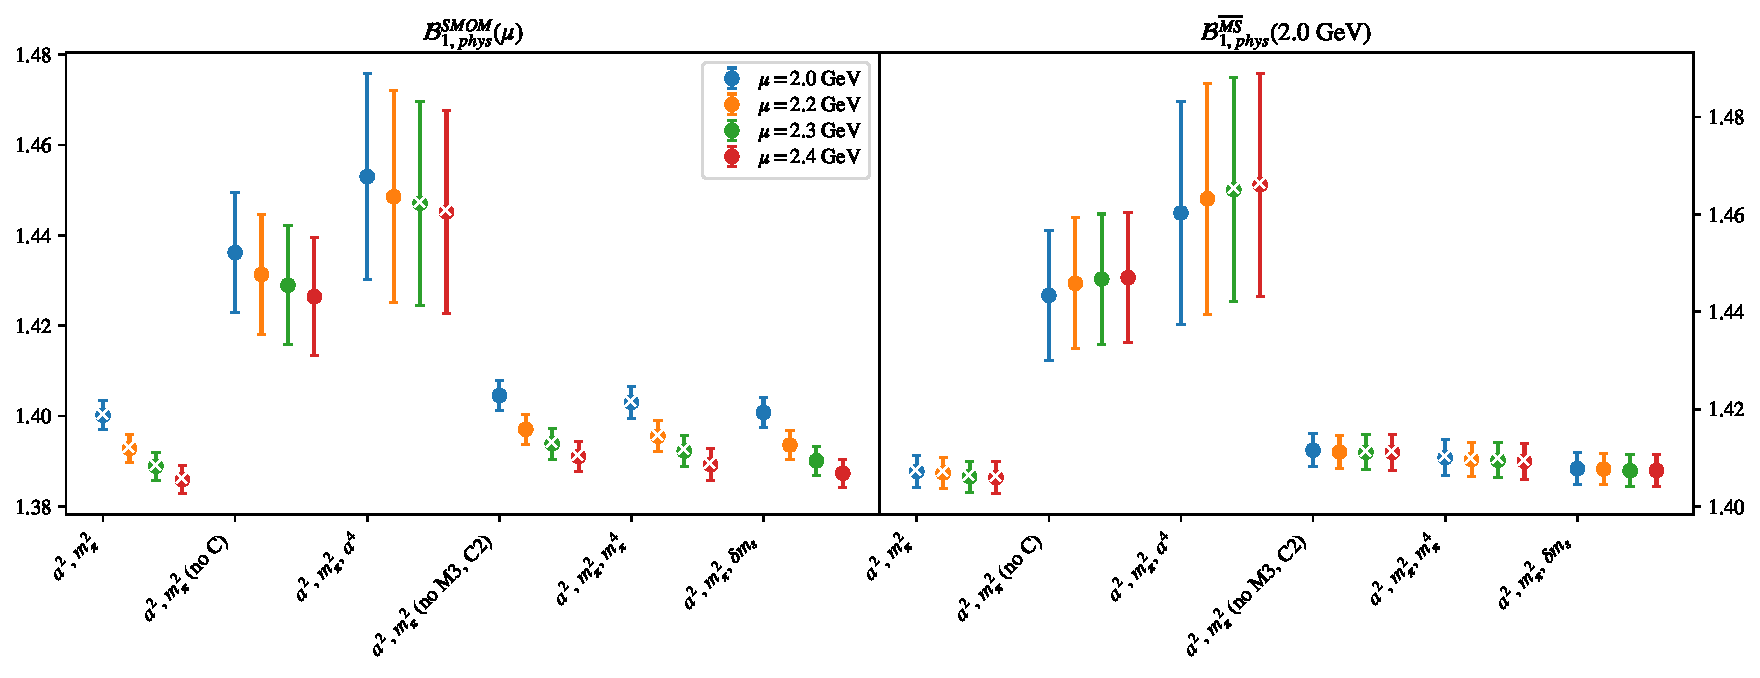
\includegraphics[page=1, width=1.1\textwidth]{VVpAA/NPR/fit_summary_bag.pdf}
\caption{$\mathcal{B}_{1}$\\(left) $\mathcal{B}_{phys}$ in RI/SMOM scheme from fit variations (fits with $p$-value $<0.05$ marked with ``$\times$"). \\(right) $\mathcal{B}_{phys}$ in $\overline{MS}$ computed using $\mathcal{B}^{\overline{MS}} = R^{\overline{MS}\leftarrow SMOM}(2.0)\sigma_{npt}(2.0,\mu) \mathcal{B}^{SMOM}(\mu)$.}
\end{figure}
\clearpage
\begin{figure}
\centering
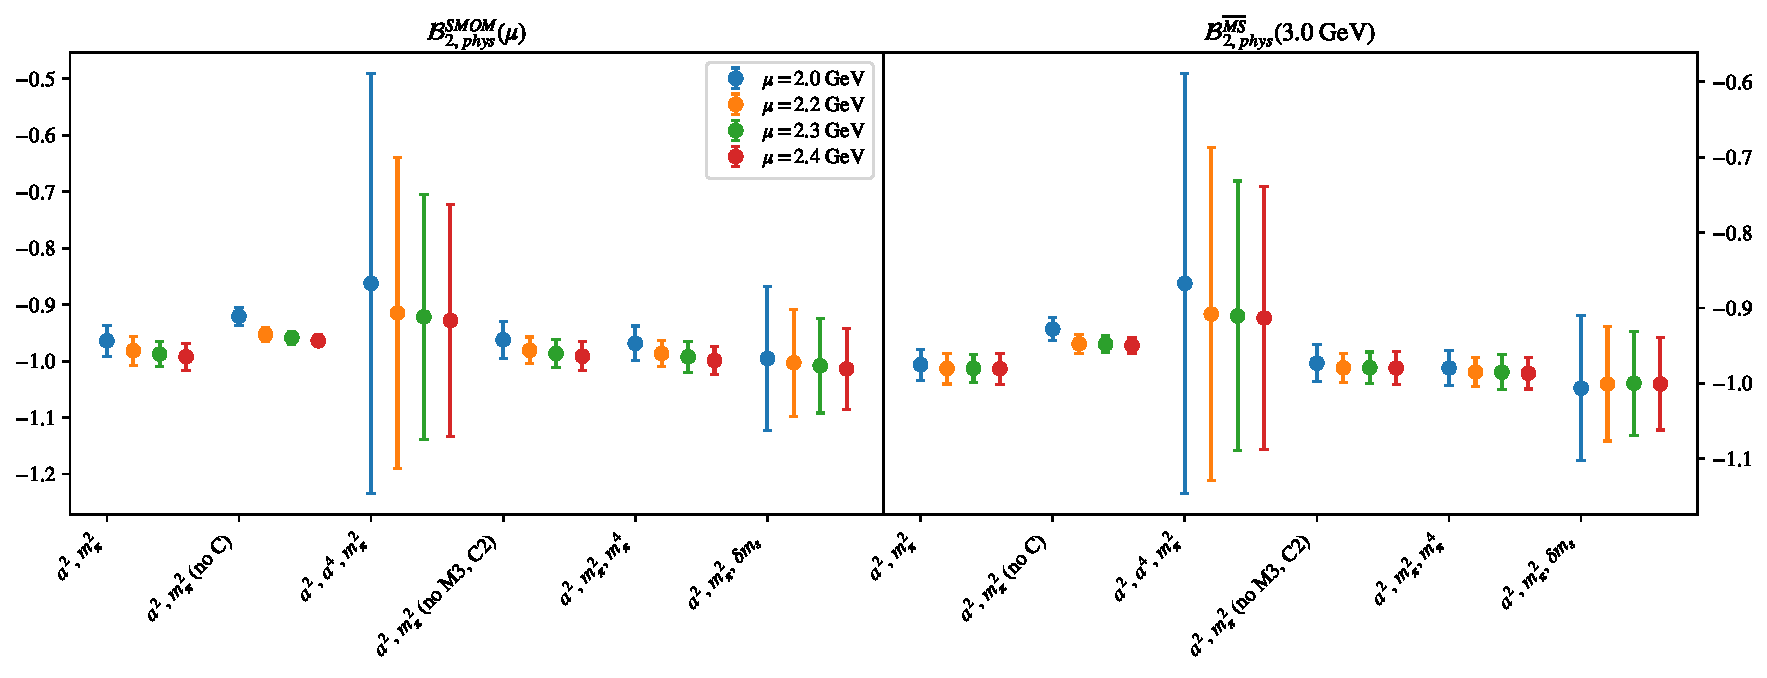
\includegraphics[page=1, width=1.1\textwidth]{VVmAA/NPR/fit_summary_bag.pdf}
\caption{$\mathcal{B}_{2}$\\(left) $\mathcal{B}_{phys}$ in RI/SMOM scheme from fit variations (fits with $p$-value $<0.05$ marked with ``$\times$"). \\(right) $\mathcal{B}_{phys}$ in $\overline{MS}$ computed using $\mathcal{B}^{\overline{MS}} = R^{\overline{MS}\leftarrow SMOM}(3.0)\sigma_{npt}(3.0,\mu) \mathcal{B}^{SMOM}(\mu)$.}
\end{figure}
\clearpage
\begin{figure}
\centering
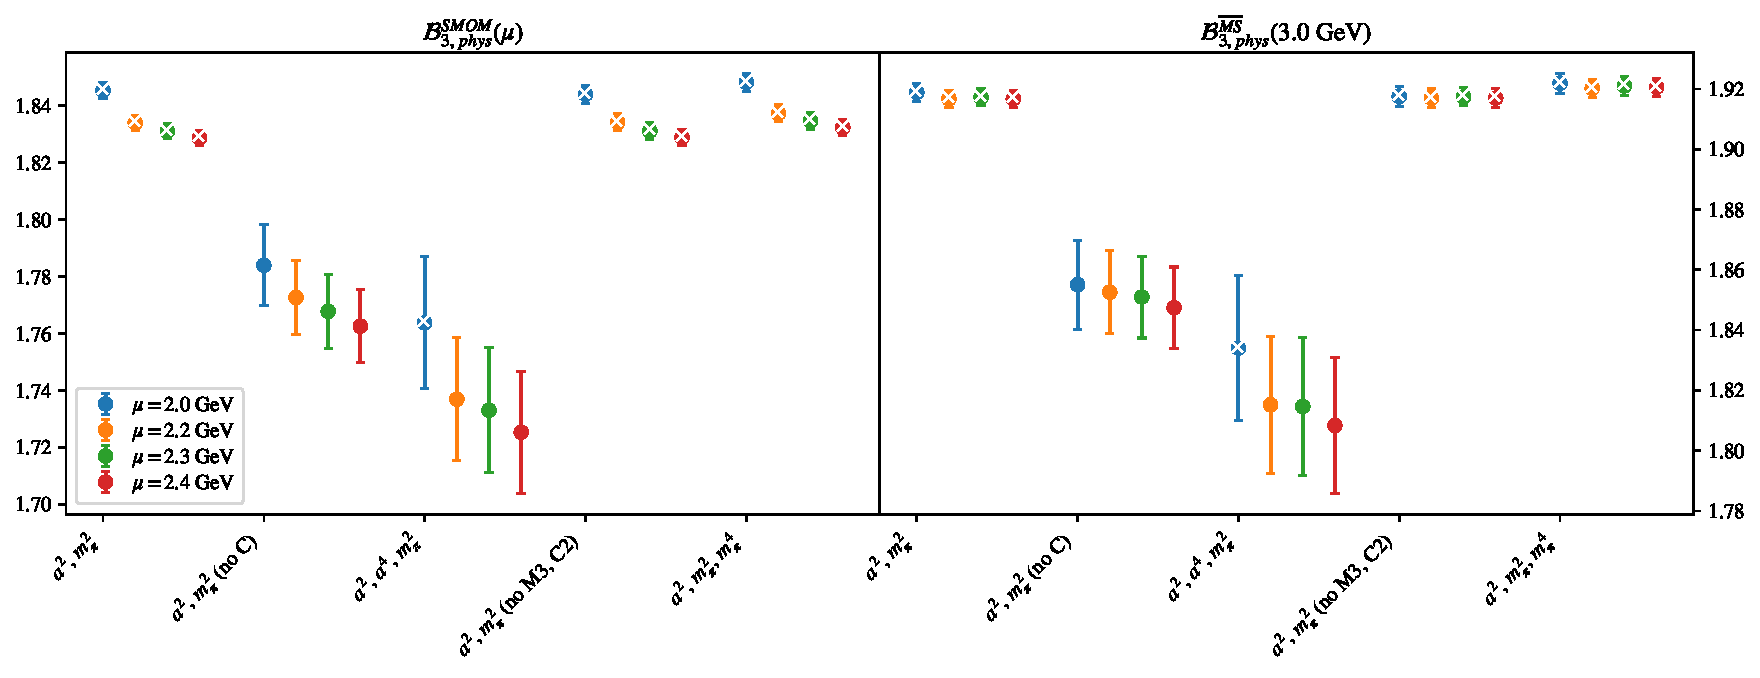
\includegraphics[page=1, width=1.1\textwidth]{SSmPP/NPR/fit_summary_bag.pdf}
\caption{$\mathcal{B}_{3}$\\(left) $\mathcal{B}_{phys}$ in RI/SMOM scheme from fit variations (fits with $p$-value $<0.05$ marked with ``$\times$"). \\(right) $\mathcal{B}_{phys}$ in $\overline{MS}$ computed using $\mathcal{B}^{\overline{MS}} = R^{\overline{MS}\leftarrow SMOM}(3.0)\sigma_{npt}(3.0,\mu) \mathcal{B}^{SMOM}(\mu)$.}
\end{figure}
\clearpage
\begin{figure}
\centering
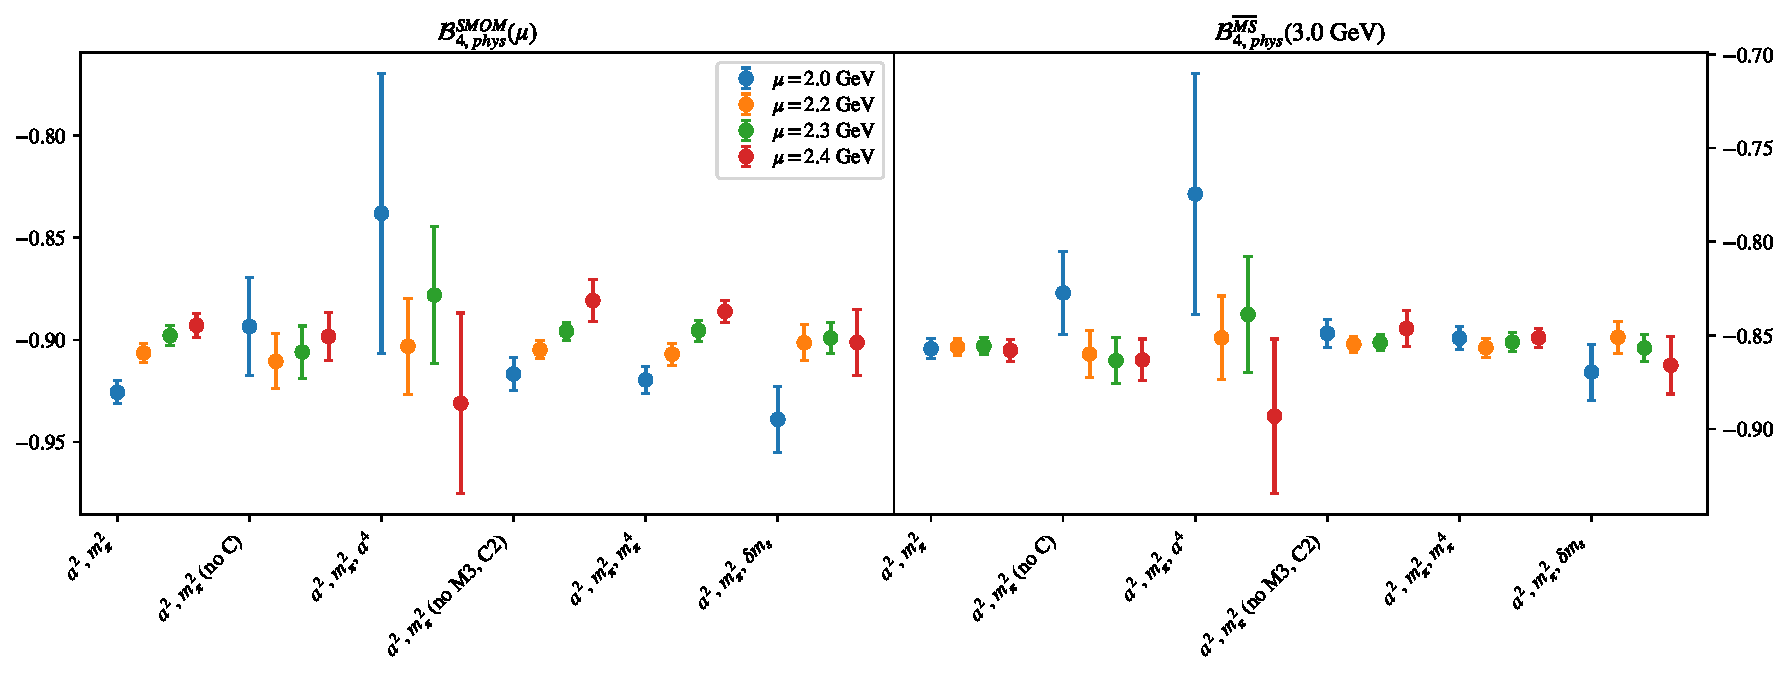
\includegraphics[page=1, width=1.1\textwidth]{SSpPP/NPR/fit_summary_bag.pdf}
\caption{$\mathcal{B}_{4}$\\(left) $\mathcal{B}_{phys}$ in RI/SMOM scheme from fit variations (fits with $p$-value $<0.05$ marked with ``$\times$"). \\(right) $\mathcal{B}_{phys}$ in $\overline{MS}$ computed using $\mathcal{B}^{\overline{MS}} = R^{\overline{MS}\leftarrow SMOM}(3.0)\sigma_{npt}(3.0,\mu) \mathcal{B}^{SMOM}(\mu)$.}
\end{figure}
\clearpage
\begin{figure}
\centering
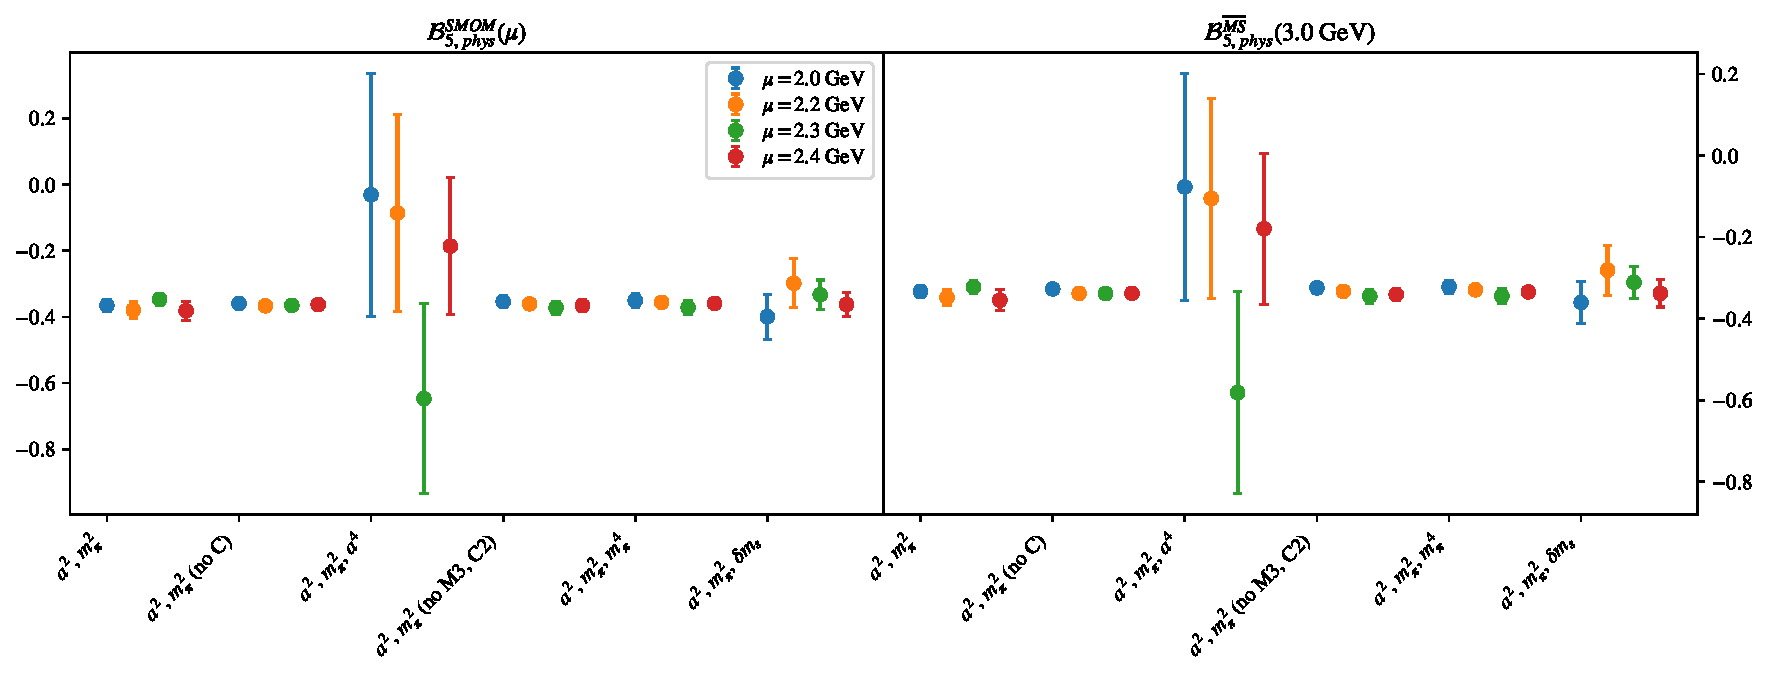
\includegraphics[page=1, width=1.1\textwidth]{TT/NPR/fit_summary_bag.pdf}
\caption{$\mathcal{B}_{5}$\\(left) $\mathcal{B}_{phys}$ in RI/SMOM scheme from fit variations (fits with $p$-value $<0.05$ marked with ``$\times$"). \\(right) $\mathcal{B}_{phys}$ in $\overline{MS}$ computed using $\mathcal{B}^{\overline{MS}} = R^{\overline{MS}\leftarrow SMOM}(3.0)\sigma_{npt}(3.0,\mu) \mathcal{B}^{SMOM}(\mu)$.}
\end{figure}
\clearpage
\section{$\mathcal{B}_1$}
\begin{table}[h!]
\begin{center}
\begin{tabular}{|c|c|c|c|c|c|}
\hline
$\mu$ (GeV) & $a^2$, $m_\pi^2$& $a^2$, $m_\pi^2$ (no C)& $a^2$, $m_\pi^2$, $a^4$& $a^2$, $m_\pi^2$ (no M3, C2)& $a^2$, $m_\pi^2$, $\delta m_s$\\
\hline
2.0& \hyperlink{VVpAA/NPR/bag_a2m2_20.pdf.1}{\textbf{1.4003(30)}: 2.547 (0.026)} & \hyperlink{VVpAA/NPR/bag_a2m2noC_20.pdf.1}{\textbf{1.434(12)}: 0.255 (0.775)} & \hyperlink{VVpAA/NPR/bag_a2a4m2_20.pdf.1}{\textbf{1.451(22)}: 1.868 (0.113)} & \hyperlink{VVpAA/NPR/bag_a2m2mcut_20.pdf.1}{\textbf{1.4043(33)}: 2.053 (0.104)} & \hyperlink{VVpAA/NPR/bag_a2m2delm_20.pdf.1}{\textbf{1.4005(31)}: 1.25 (0.287)}\\
2.2& \hyperlink{VVpAA/NPR/bag_a2m2_22.pdf.1}{\textbf{1.3933(29)}: 3.059 (0.009)} & \hyperlink{VVpAA/NPR/bag_a2m2noC_22.pdf.1}{\textbf{1.430(12)}: 0.288 (0.75)} & \hyperlink{VVpAA/NPR/bag_a2a4m2_22.pdf.1}{\textbf{1.450(22)}: 2.131 (0.074)} & \hyperlink{VVpAA/NPR/bag_a2m2mcut_22.pdf.1}{\textbf{1.3976(32)}: 2.518 (0.056)} & \hyperlink{VVpAA/NPR/bag_a2m2delm_22.pdf.1}{\textbf{1.3936(31)}: 1.336 (0.254)}\\
2.3& \hyperlink{VVpAA/NPR/bag_a2m2_23.pdf.1}{\textbf{1.3899(29)}: 3.366 (0.005)} & \hyperlink{VVpAA/NPR/bag_a2m2noC_23.pdf.1}{\textbf{1.429(12)}: 0.33 (0.719)} & \hyperlink{VVpAA/NPR/bag_a2a4m2_23.pdf.1}{\textbf{1.448(22)}: 2.397 (0.048)} & \hyperlink{VVpAA/NPR/bag_a2m2mcut_23.pdf.1}{\textbf{1.3944(33)}: 2.771 (0.04)} & \hyperlink{VVpAA/NPR/bag_a2m2delm_23.pdf.1}{\textbf{1.3902(31)}: 1.529 (0.191)}\\
2.4& \hyperlink{VVpAA/NPR/bag_a2m2_24.pdf.1}{\textbf{1.3868(29)}: 3.569 (0.003)} & \hyperlink{VVpAA/NPR/bag_a2m2noC_24.pdf.1}{\textbf{1.426(12)}: 0.347 (0.707)} & \hyperlink{VVpAA/NPR/bag_a2a4m2_24.pdf.1}{\textbf{1.446(22)}: 2.594 (0.035)} & \hyperlink{VVpAA/NPR/bag_a2m2mcut_24.pdf.1}{\textbf{1.3915(33)}: 2.877 (0.035)} & \hyperlink{VVpAA/NPR/bag_a2m2delm_24.pdf.1}{\textbf{1.3872(31)}: 1.647 (0.159)}\\
\hline
\end{tabular}
\caption{Physical point value from chiral and continuum extrapolation at renormalisation scale $\mu$. Entries are \textbf{value(error)}: $\chi^2/\text{DOF}$ ($p$-value).}
\end{center}
\end{table}
\begin{table}[h!]
\begin{center}
\begin{tabular}{|c c|c|c|c|c|c|}
\hline
$\mu$ (GeV) &  & $a^2$, $m_\pi^2$& $a^2$, $m_\pi^2$ (no C)& $a^2$, $m_\pi^2$, $a^4$& $a^2$, $m_\pi^2$ (no M3, C2)& $a^2$, $m_\pi^2$, $\delta m_s$\\
\hline
\multirow{3}{0.5in}{2.0} & $\alpha$ & 0.145(10)& -0.045(75)& -0.32(20)& 0.133(11)& 0.149(11)\\
 & $\beta$ & 0.00413(23)& 0.00353(43)& 0.00440(26)& 0.00349(37)& 0.00539(47)\\
 & $\gamma$ &  &  & 0.96(41)&  & -0.049(15)\\
\hline
\multirow{3}{0.5in}{2.2} & $\alpha$ & 0.149(10)& -0.060(75)& -0.37(20)& 0.136(11)& 0.153(11)\\
 & $\beta$ & 0.00400(22)& 0.00338(42)& 0.00430(25)& 0.00331(36)& 0.00540(46)\\
 & $\gamma$ &  &  & 1.07(41)&  & -0.054(16)\\
\hline
\multirow{3}{0.5in}{2.3} & $\alpha$ & 0.152(10)& -0.067(75)& -0.39(20)& 0.138(11)& 0.156(11)\\
 & $\beta$ & 0.00396(22)& 0.00330(41)& 0.00427(25)& 0.00324(36)& 0.00540(46)\\
 & $\gamma$ &  &  & 1.10(41)&  & -0.056(15)\\
\hline
\multirow{3}{0.5in}{2.4} & $\alpha$ & 0.154(10)& -0.068(74)& -0.40(20)& 0.139(11)& 0.157(11)\\
 & $\beta$ & 0.00393(22)& 0.00325(41)& 0.00425(25)& 0.00319(35)& 0.00541(46)\\
 & $\gamma$ &  &  & 1.12(41)&  & -0.057(15)\\
\hline
\end{tabular}
\caption{Fit values of coefficients in $Q = Q_{phys} + \mathbf{\alpha} a^2 + \mathbf{\beta}\left(\frac{m_\pi^2}{f_\pi^2}-\frac{m_{\pi,PDG}^2}{f_\pi^2}\right) + \gamma(\ldots)$}
\end{center}
\end{table}
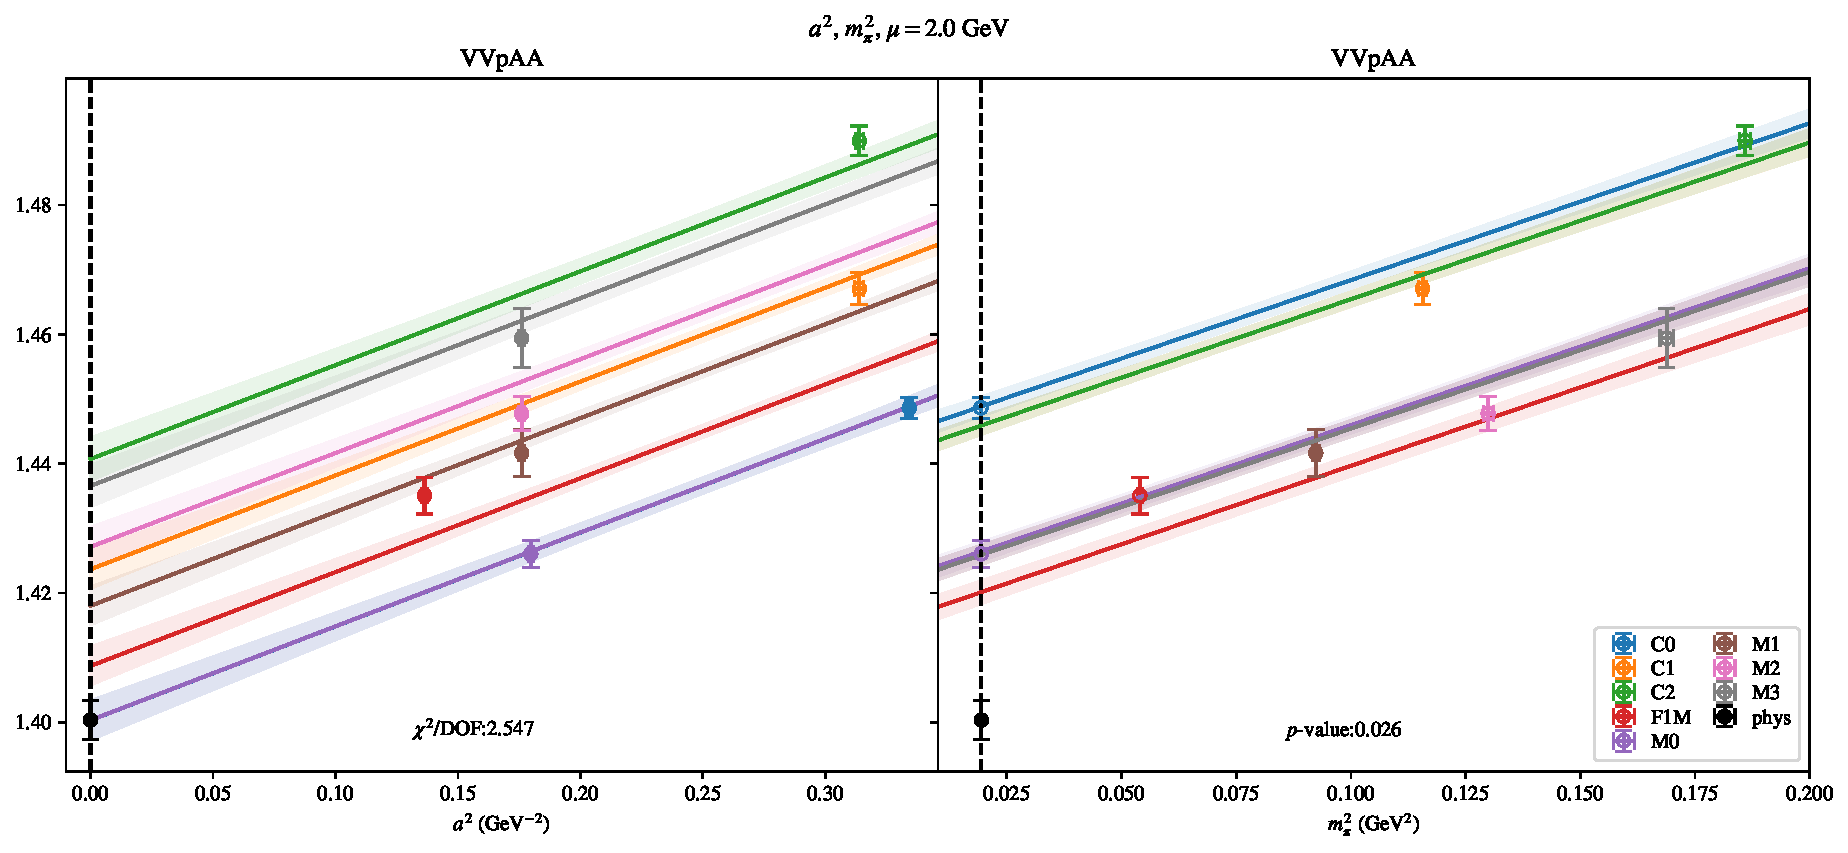
\includepdf[link, pages=-]{VVpAA/NPR/bag_a2m2_20.pdf}
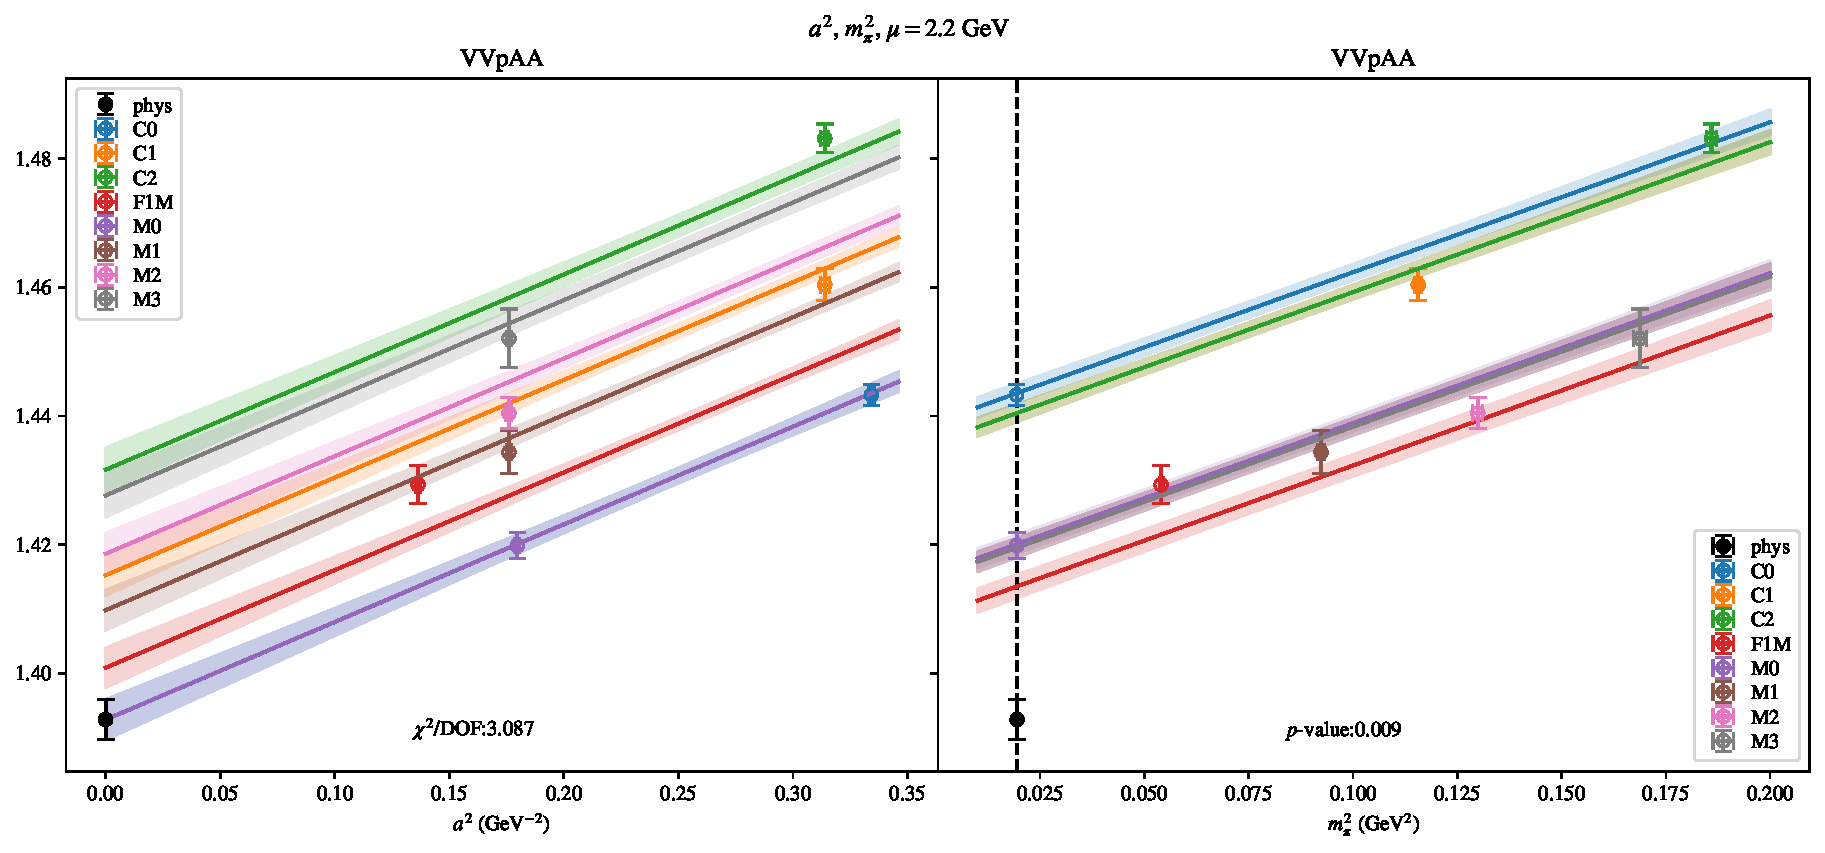
\includepdf[link, pages=-]{VVpAA/NPR/bag_a2m2_22.pdf}
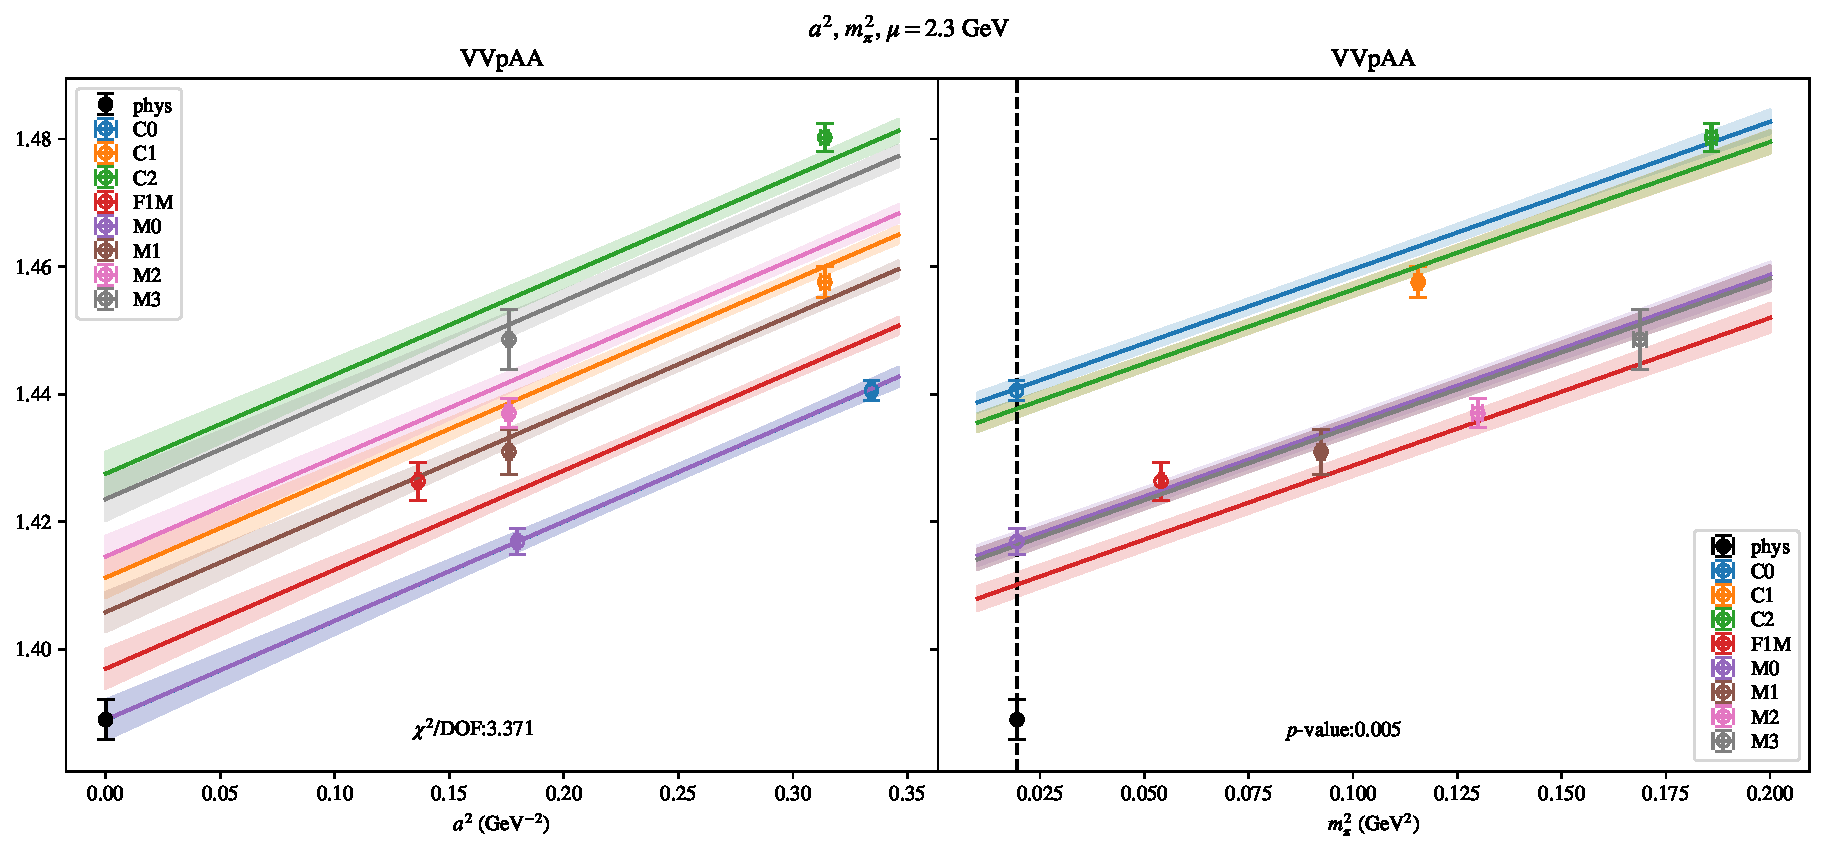
\includepdf[link, pages=-]{VVpAA/NPR/bag_a2m2_23.pdf}
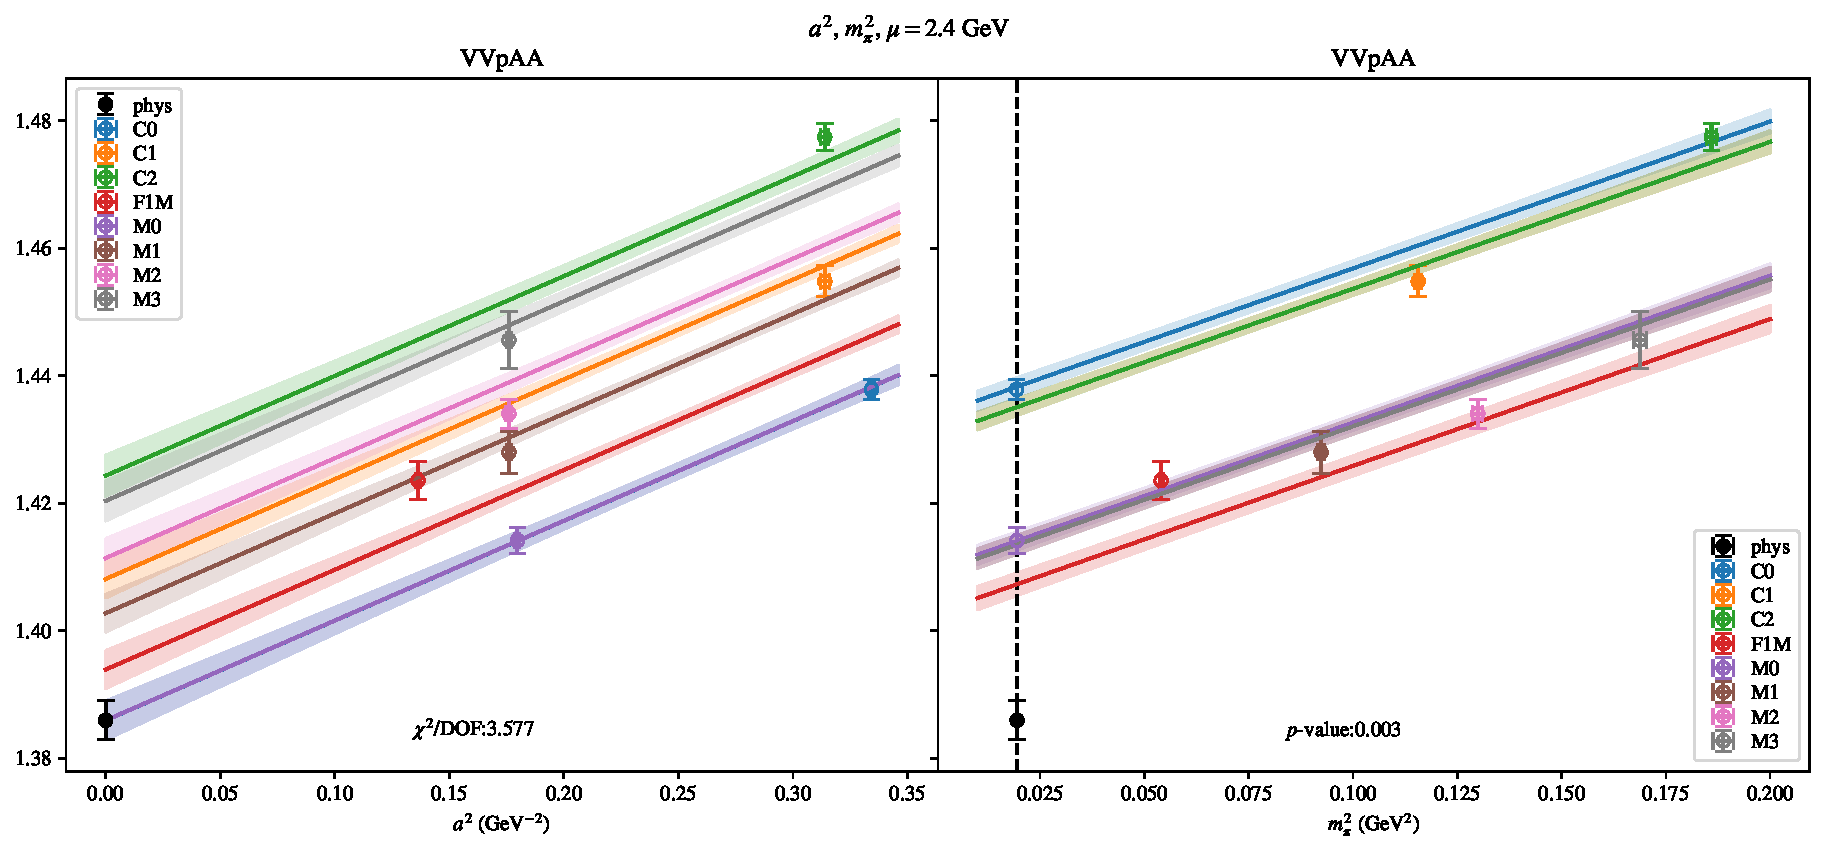
\includepdf[link, pages=-]{VVpAA/NPR/bag_a2m2_24.pdf}
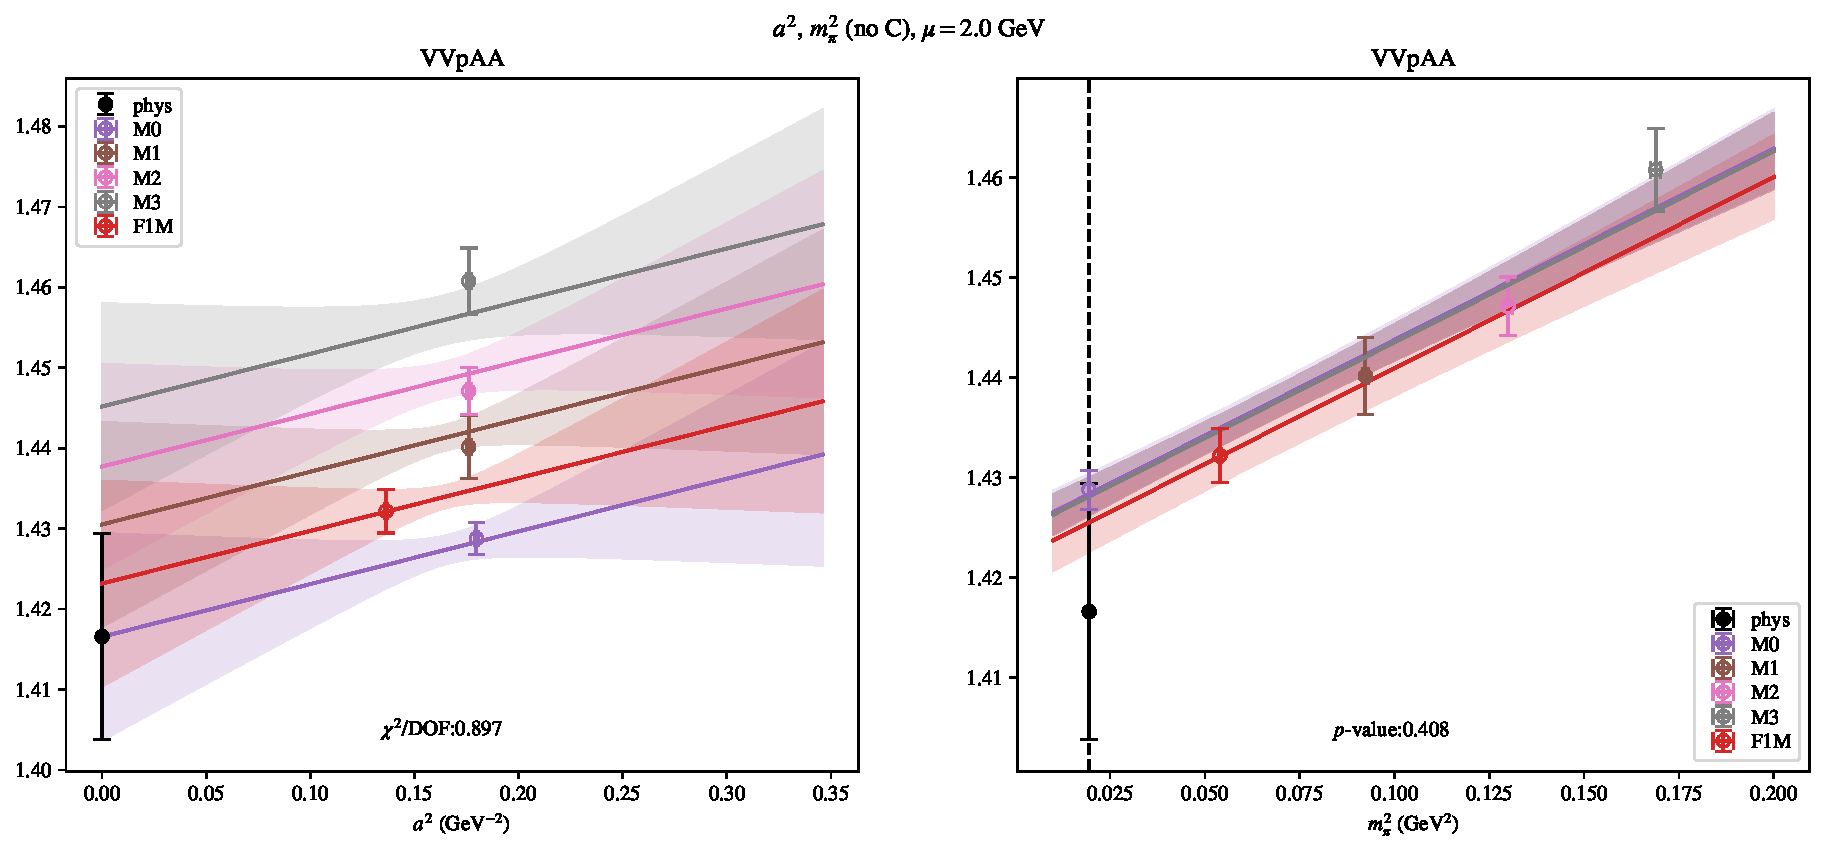
\includepdf[link, pages=-]{VVpAA/NPR/bag_a2m2noC_20.pdf}
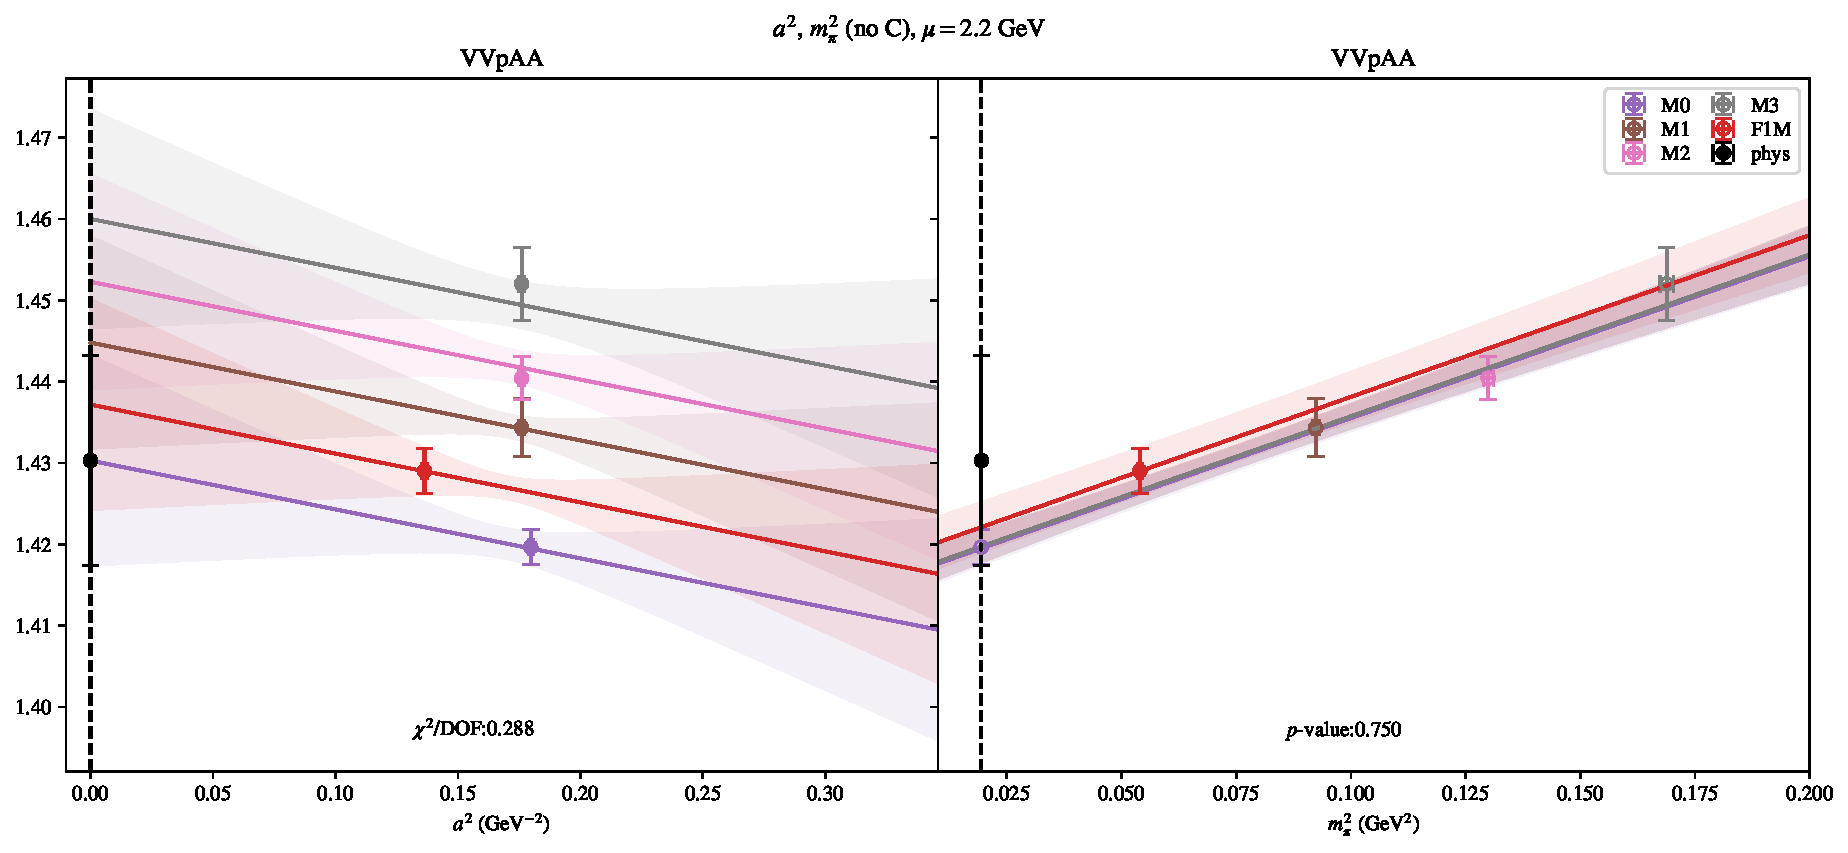
\includepdf[link, pages=-]{VVpAA/NPR/bag_a2m2noC_22.pdf}
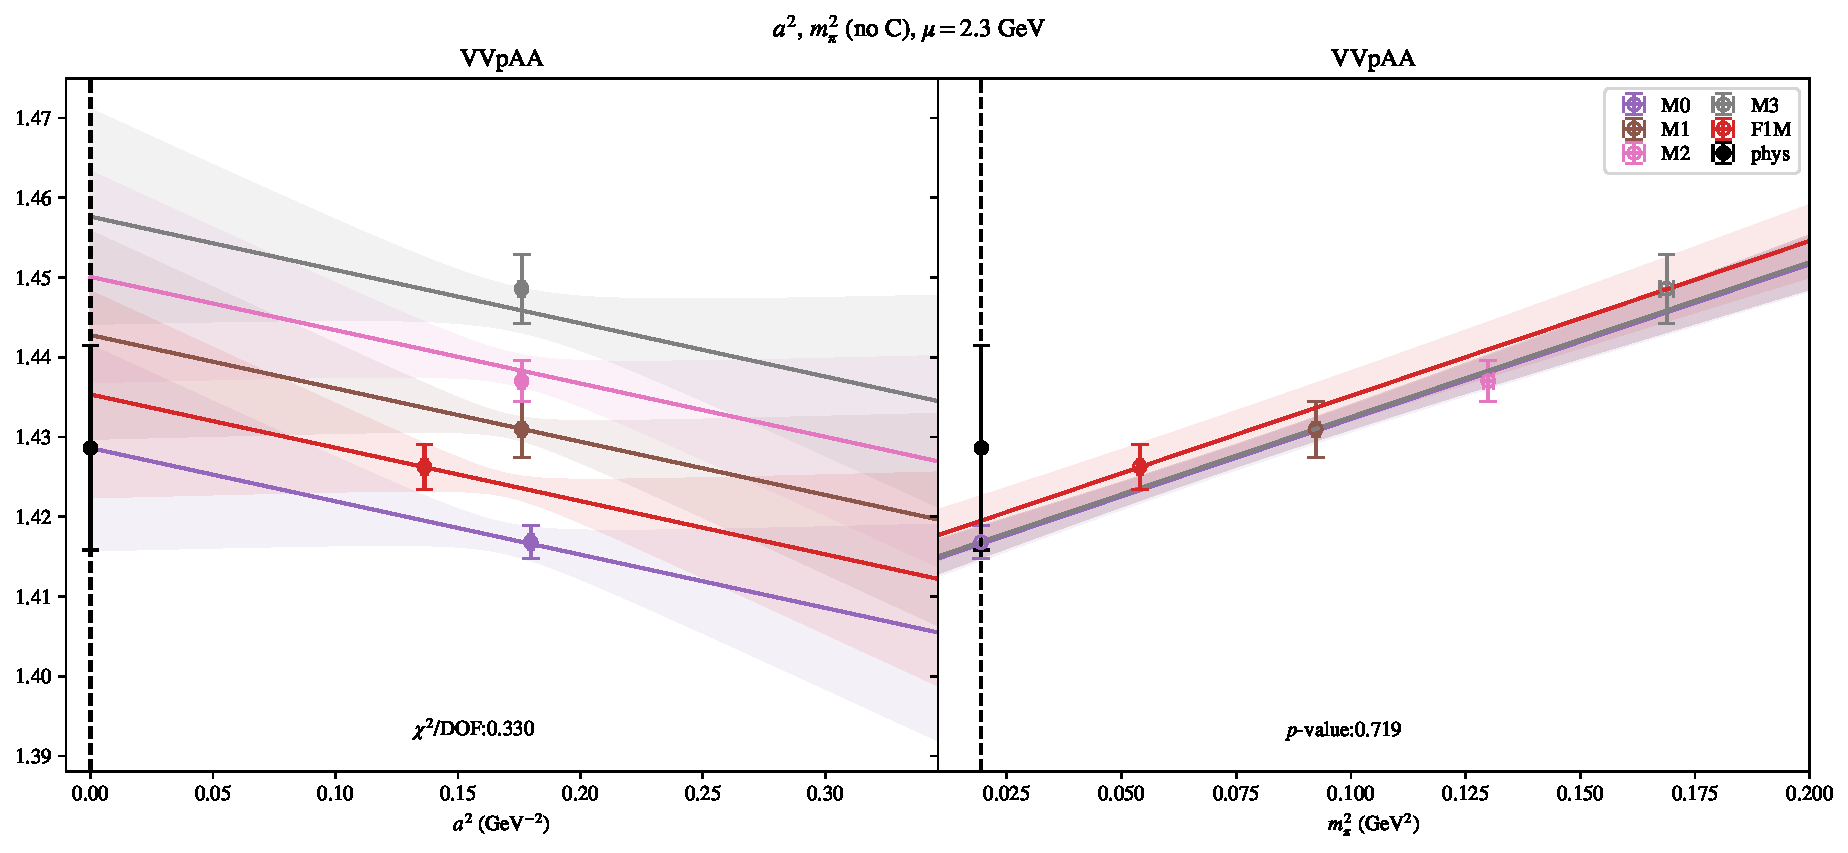
\includepdf[link, pages=-]{VVpAA/NPR/bag_a2m2noC_23.pdf}
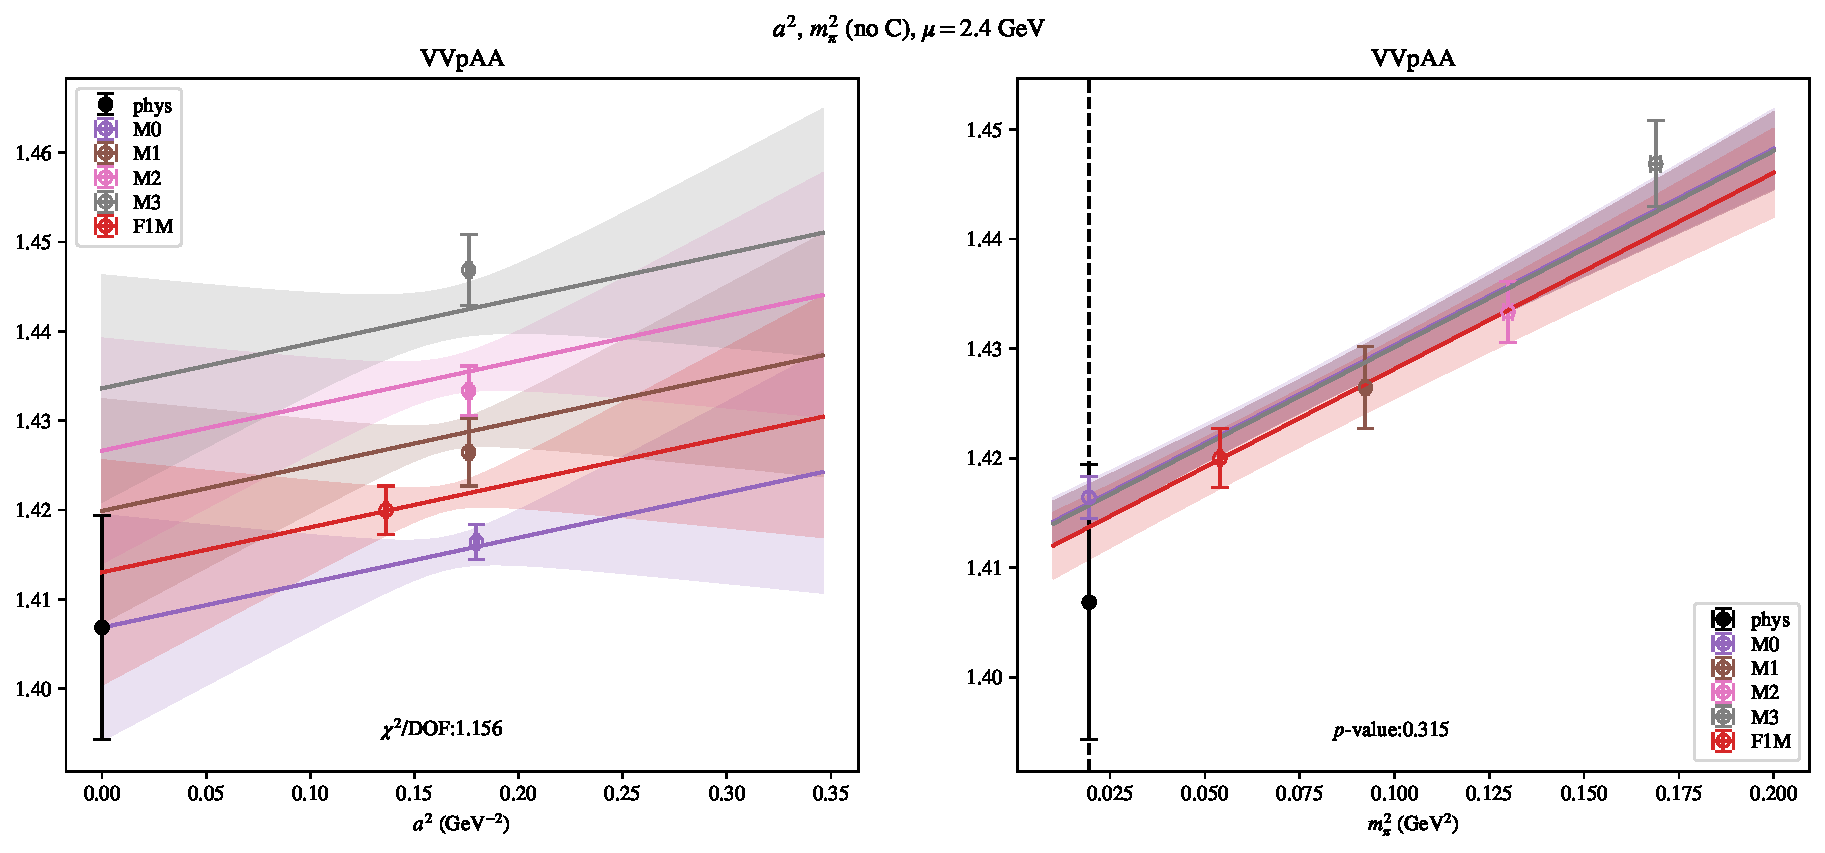
\includepdf[link, pages=-]{VVpAA/NPR/bag_a2m2noC_24.pdf}
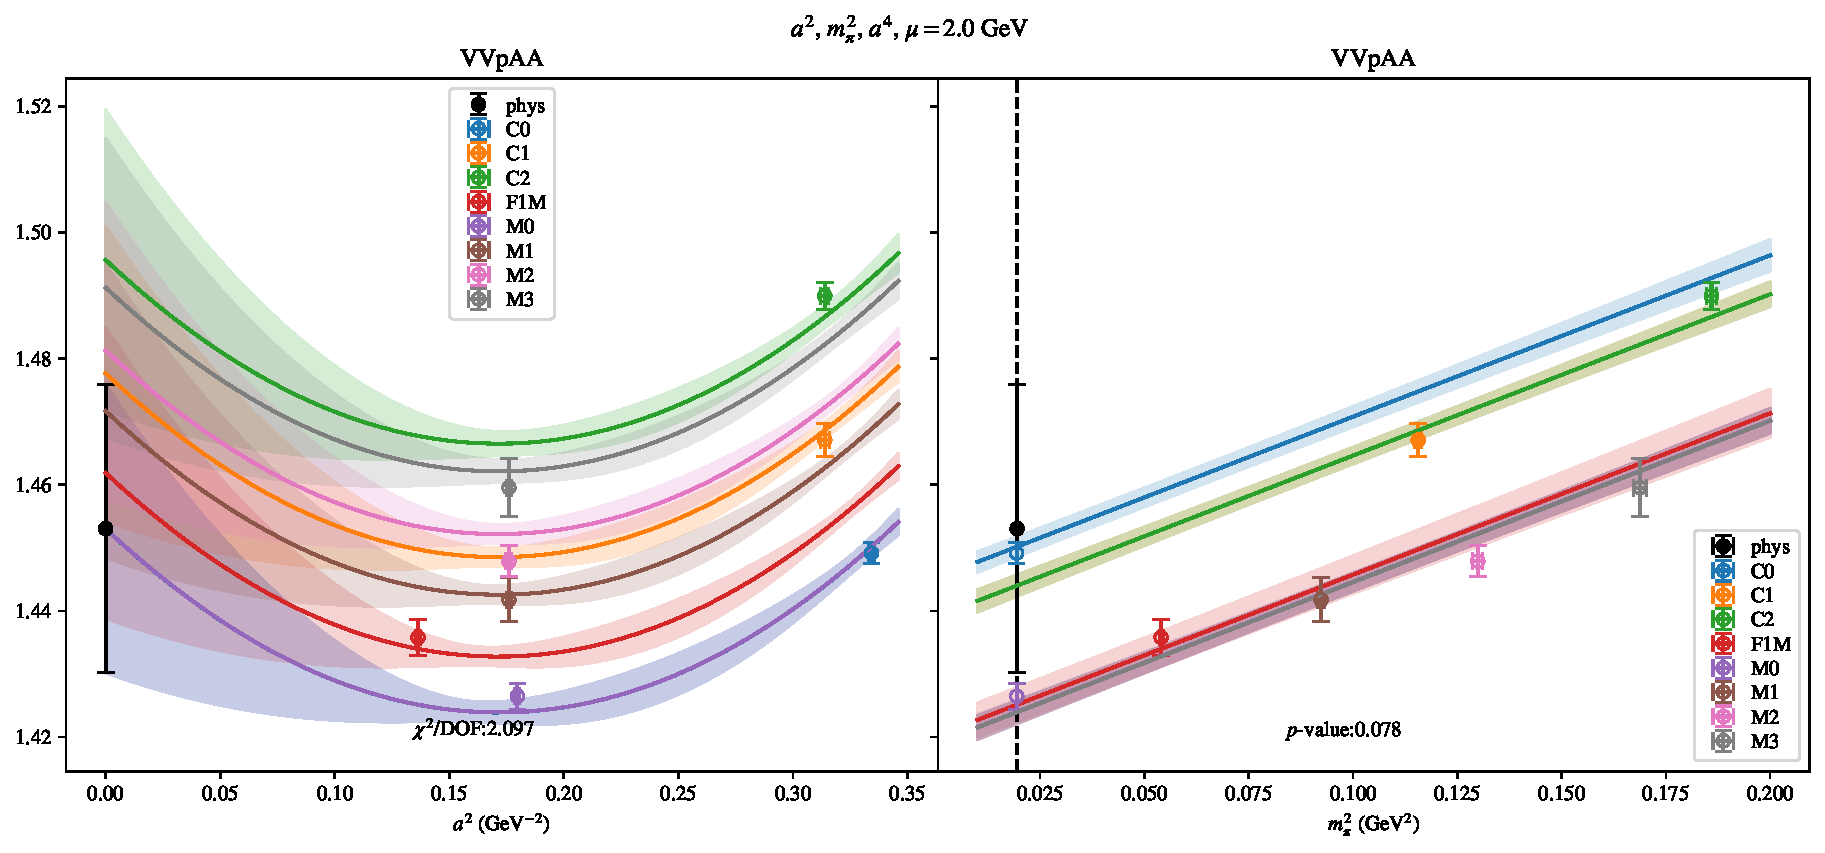
\includepdf[link, pages=-]{VVpAA/NPR/bag_a2a4m2_20.pdf}
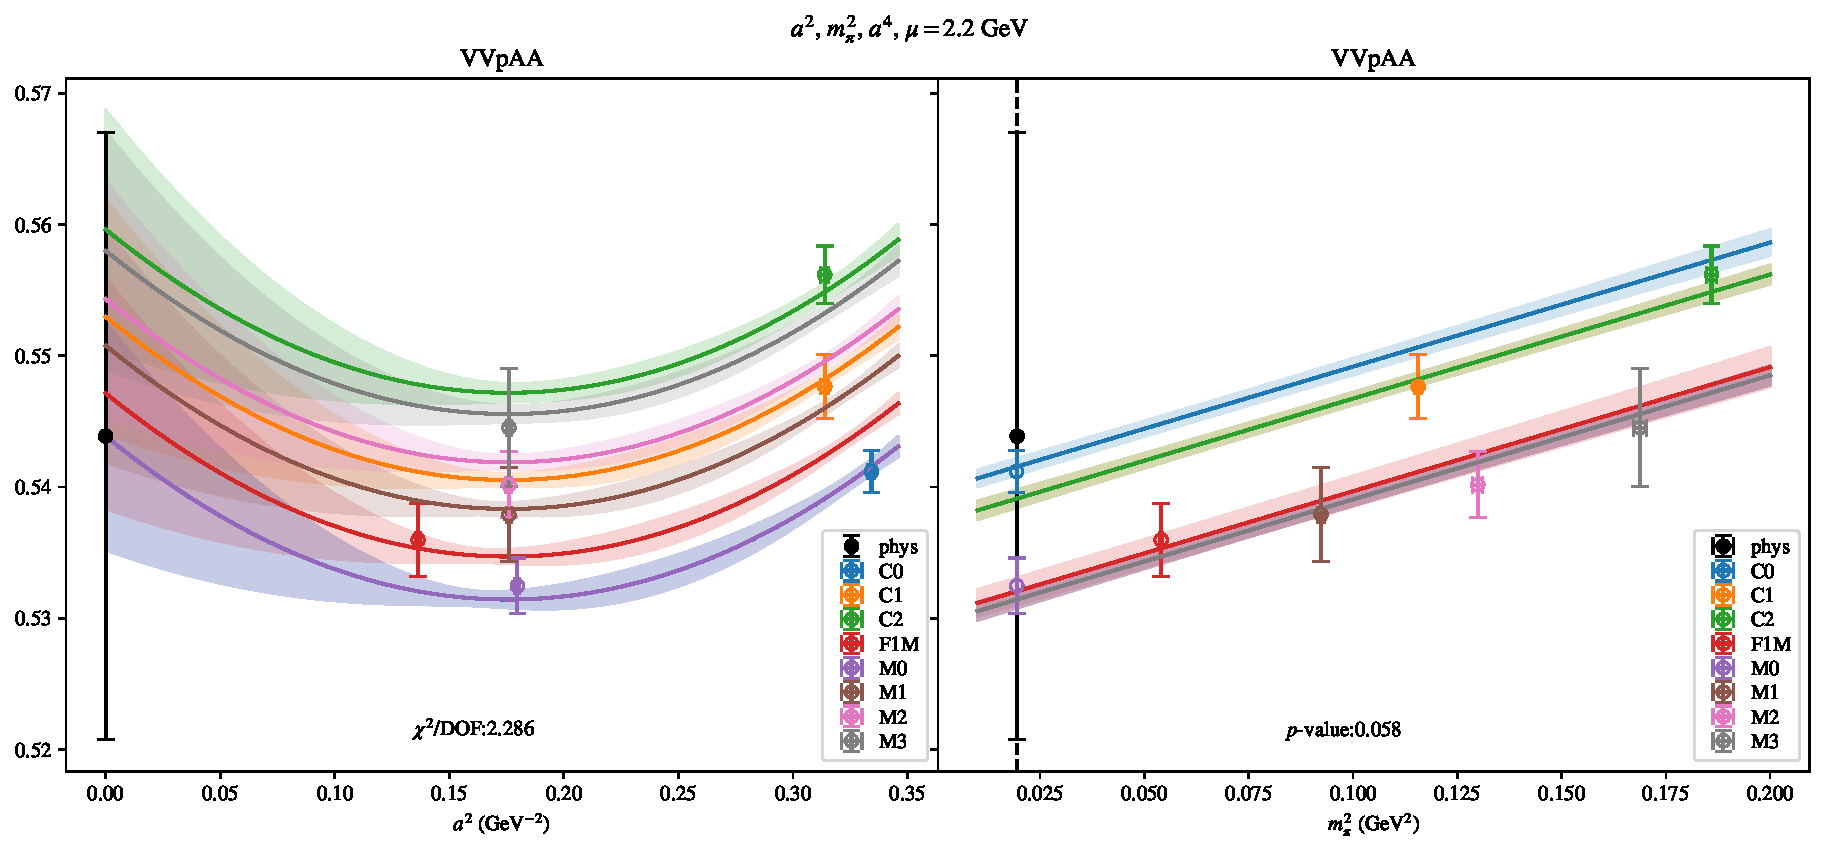
\includepdf[link, pages=-]{VVpAA/NPR/bag_a2a4m2_22.pdf}
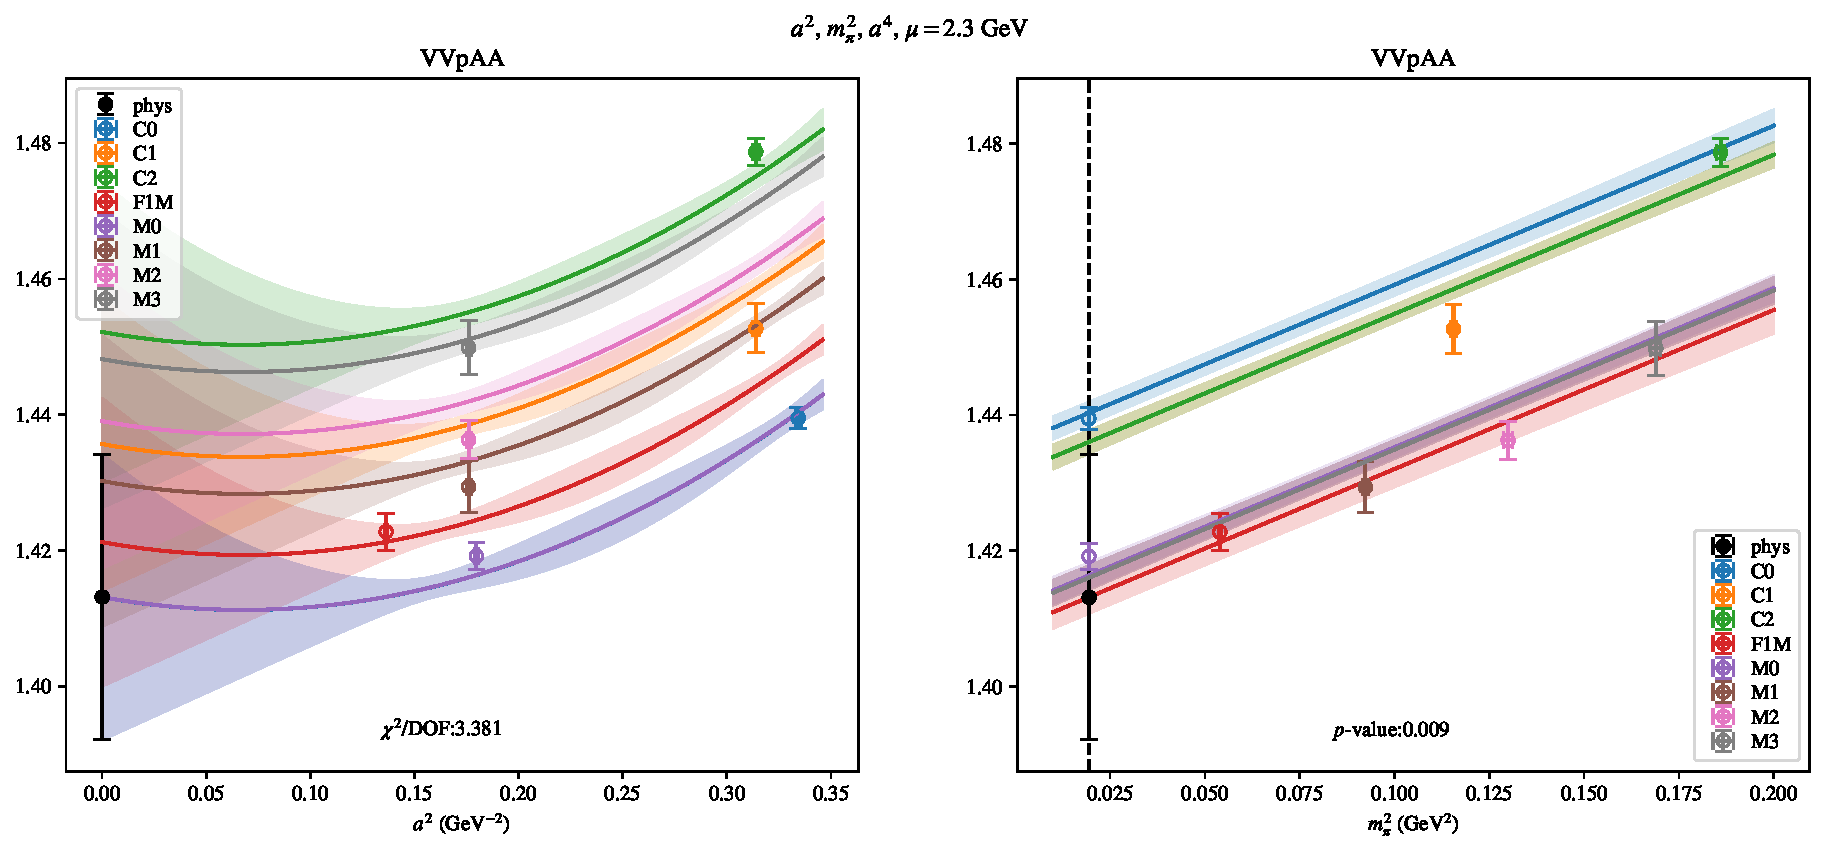
\includepdf[link, pages=-]{VVpAA/NPR/bag_a2a4m2_23.pdf}
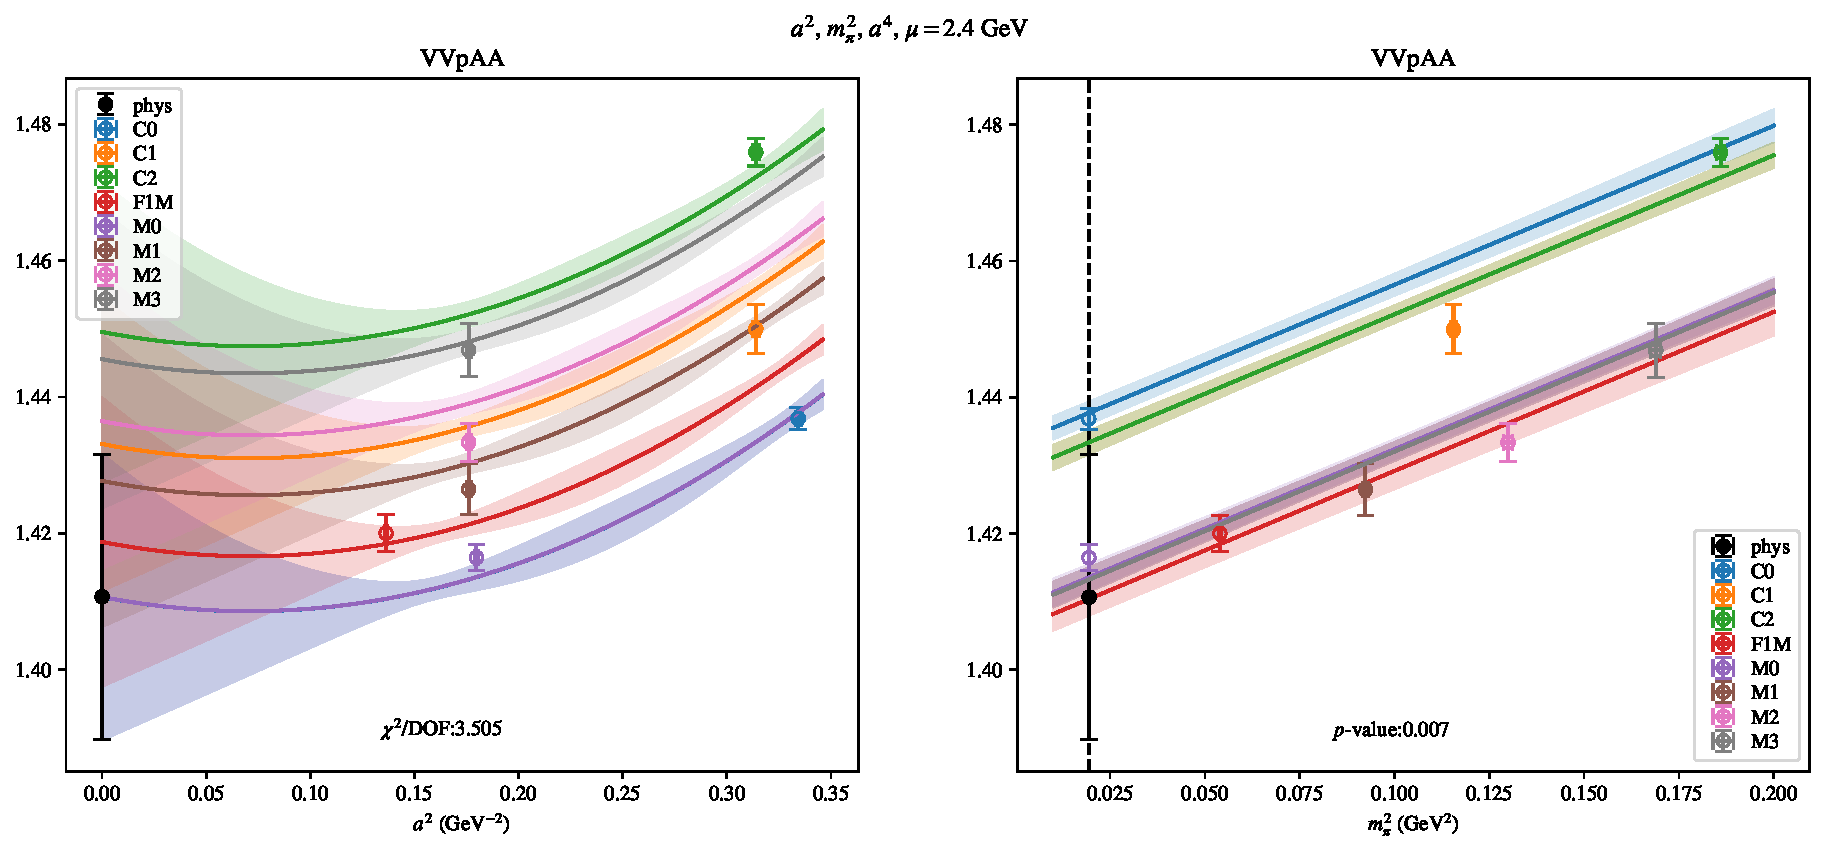
\includepdf[link, pages=-]{VVpAA/NPR/bag_a2a4m2_24.pdf}
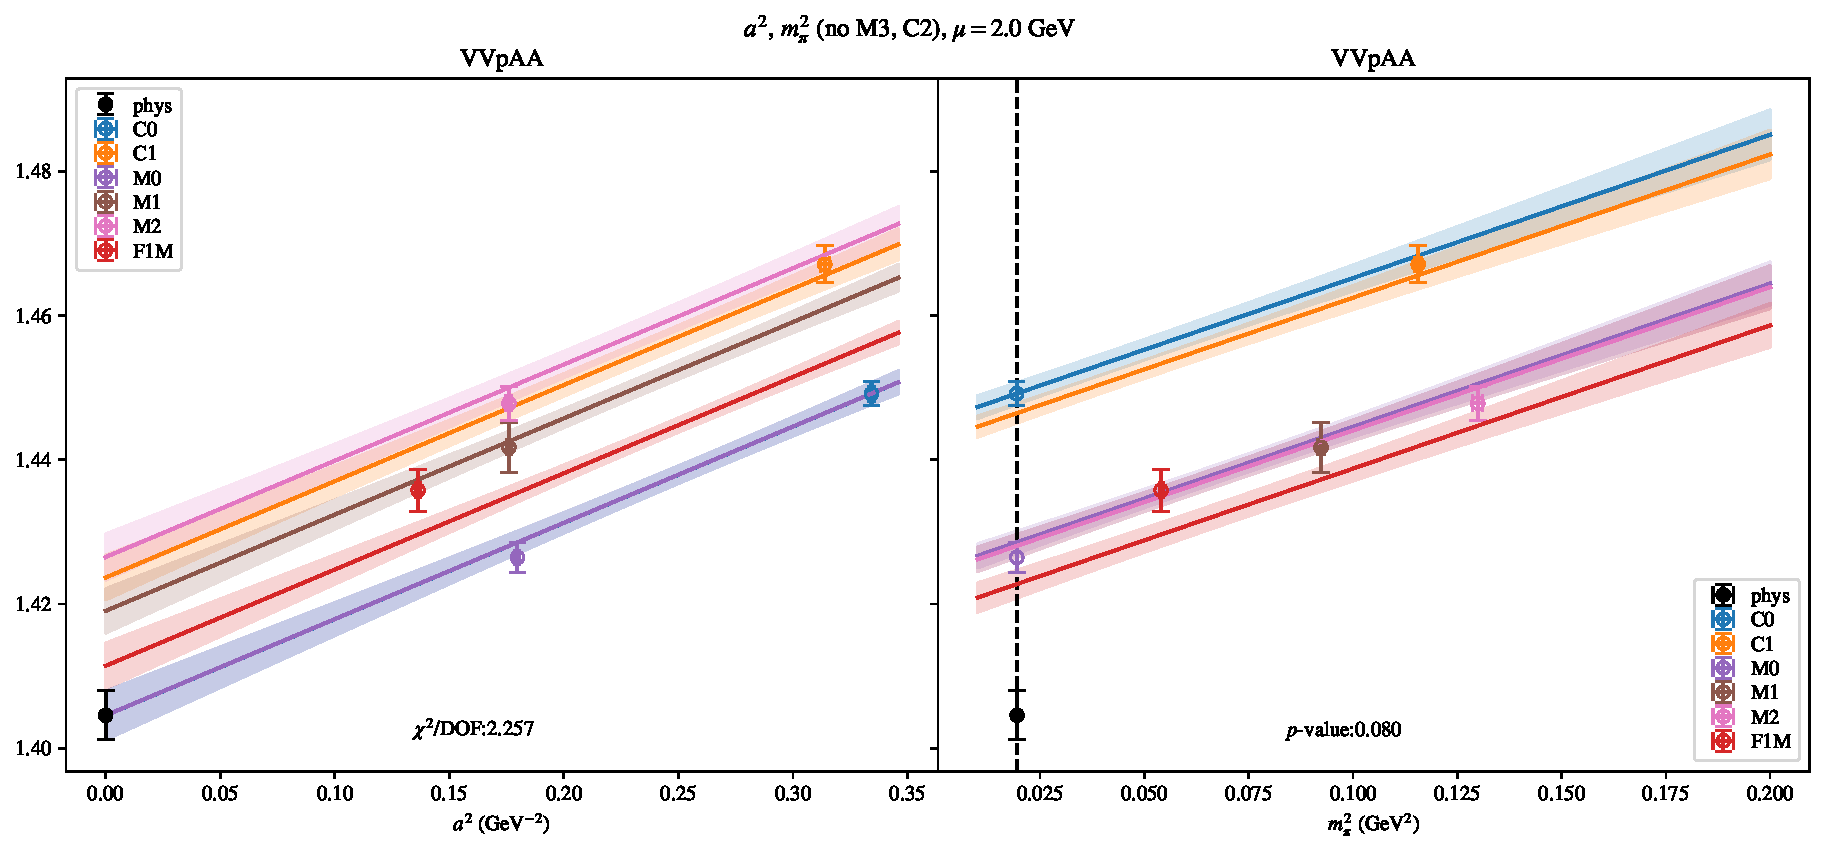
\includepdf[link, pages=-]{VVpAA/NPR/bag_a2m2mcut_20.pdf}
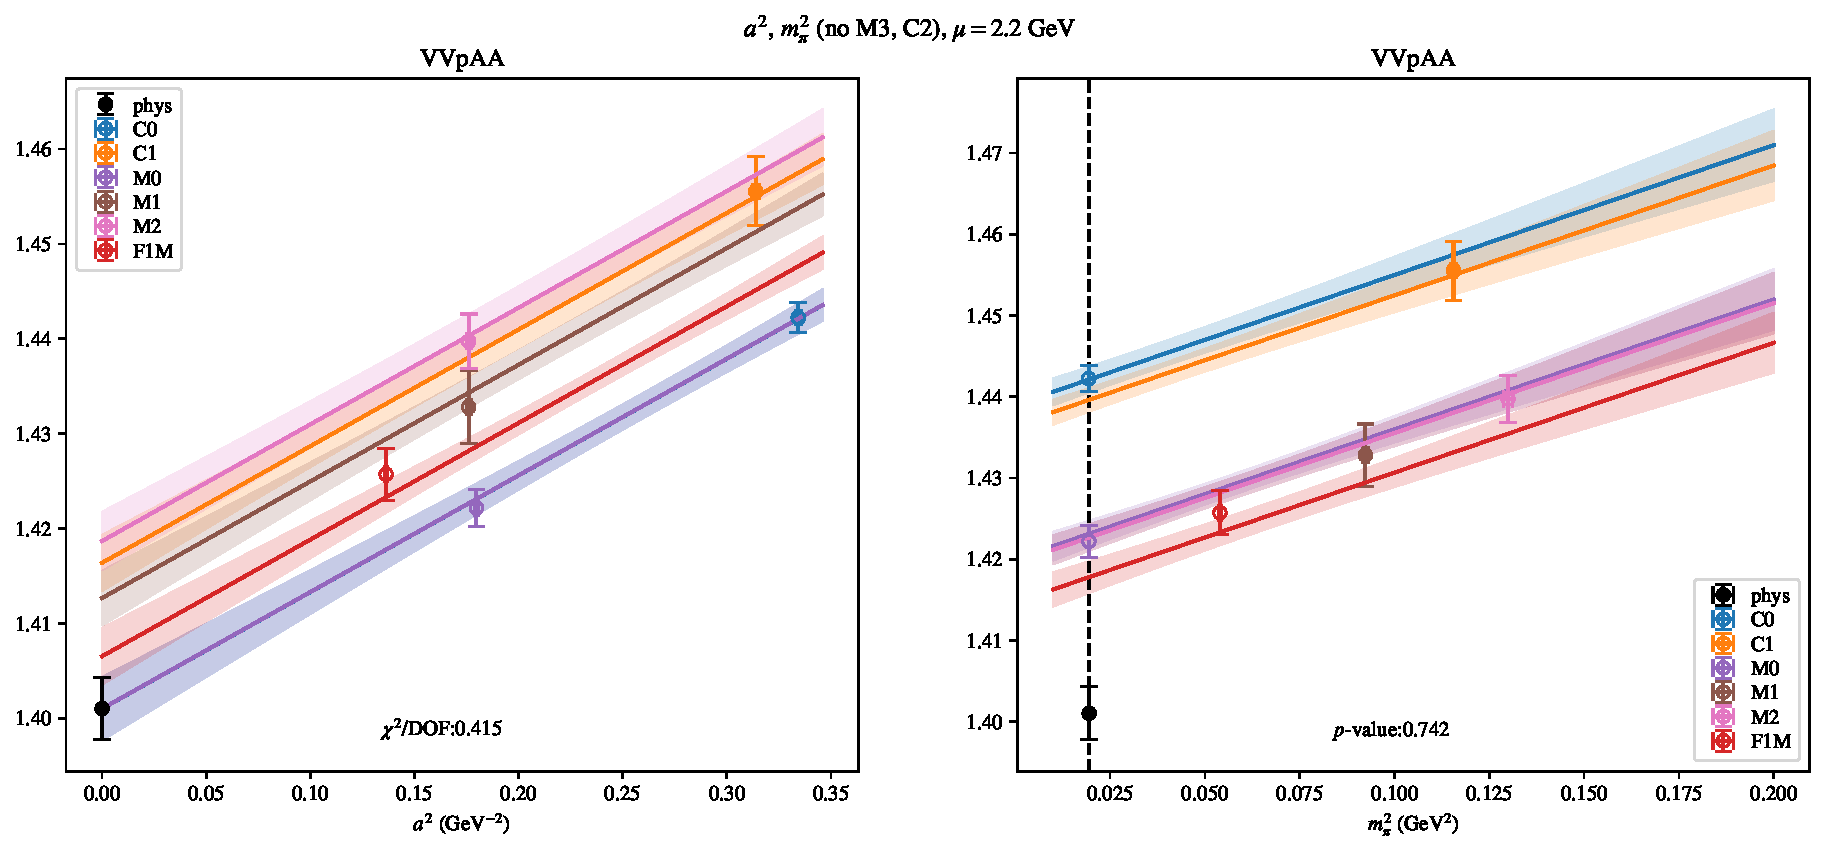
\includepdf[link, pages=-]{VVpAA/NPR/bag_a2m2mcut_22.pdf}
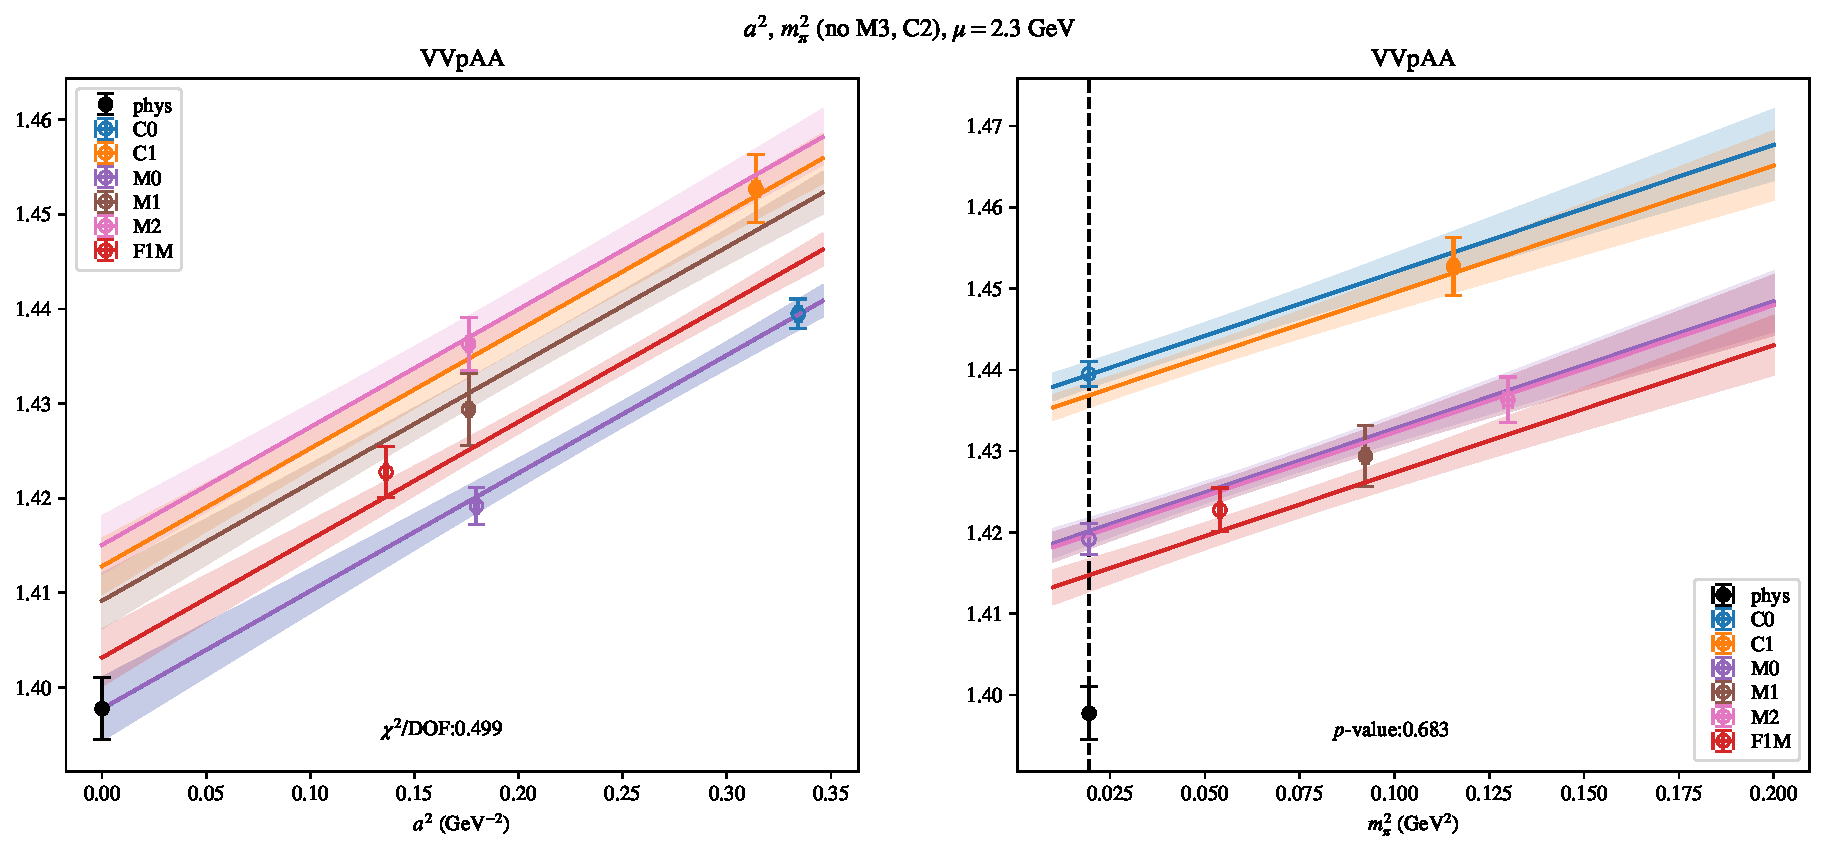
\includepdf[link, pages=-]{VVpAA/NPR/bag_a2m2mcut_23.pdf}
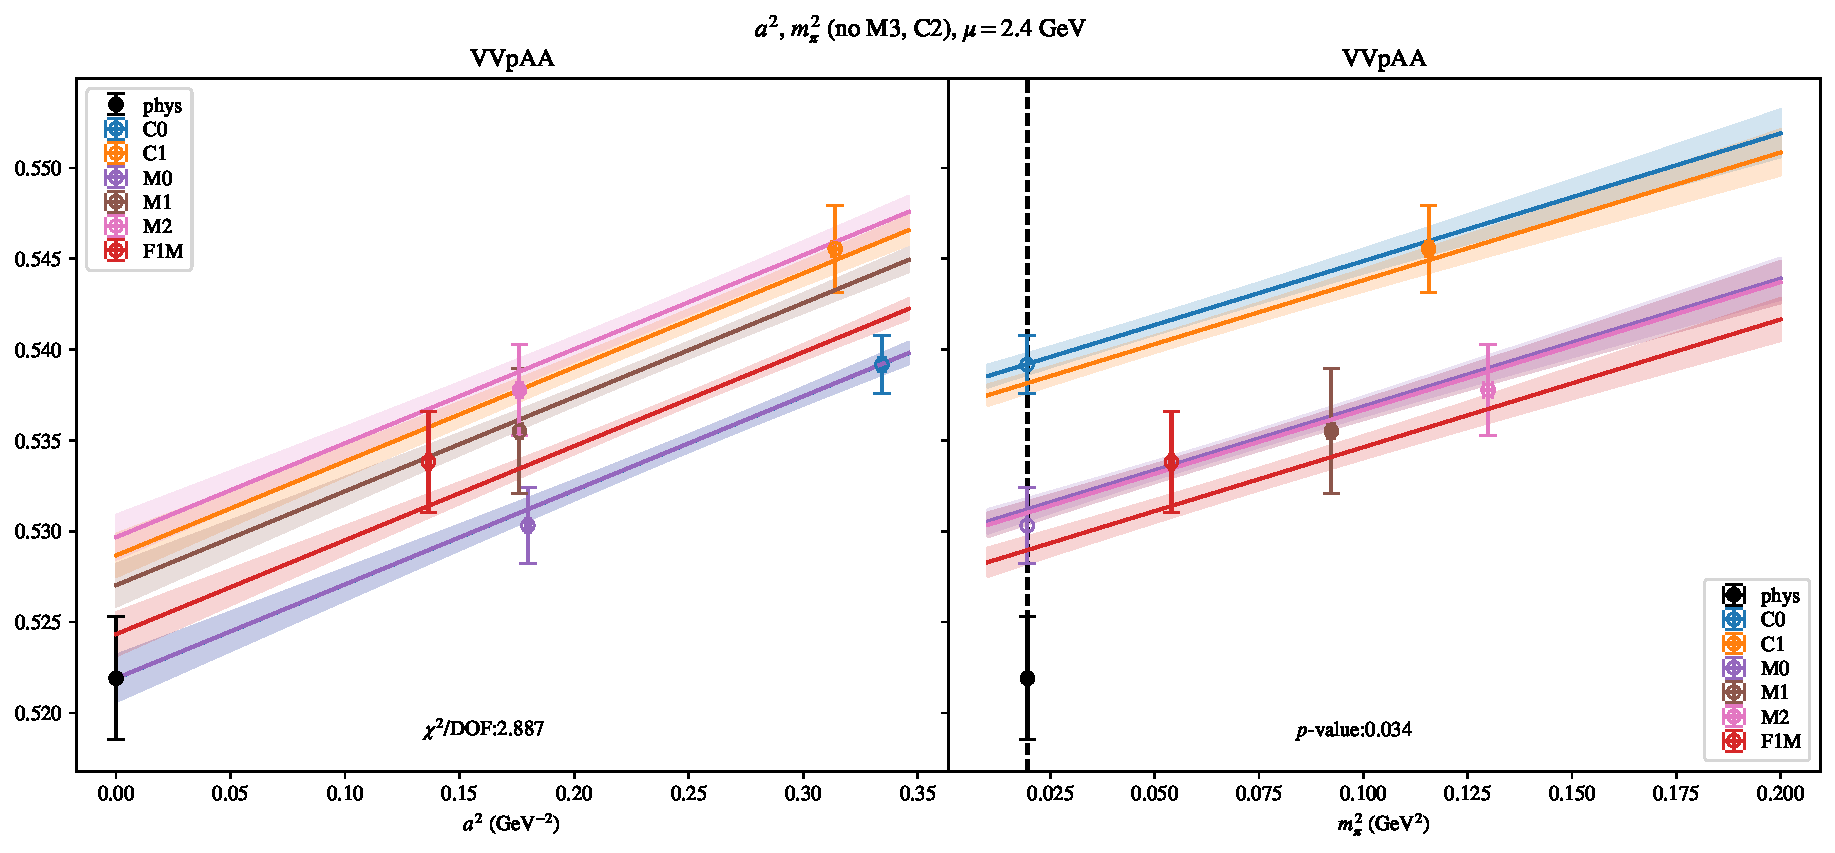
\includepdf[link, pages=-]{VVpAA/NPR/bag_a2m2mcut_24.pdf}
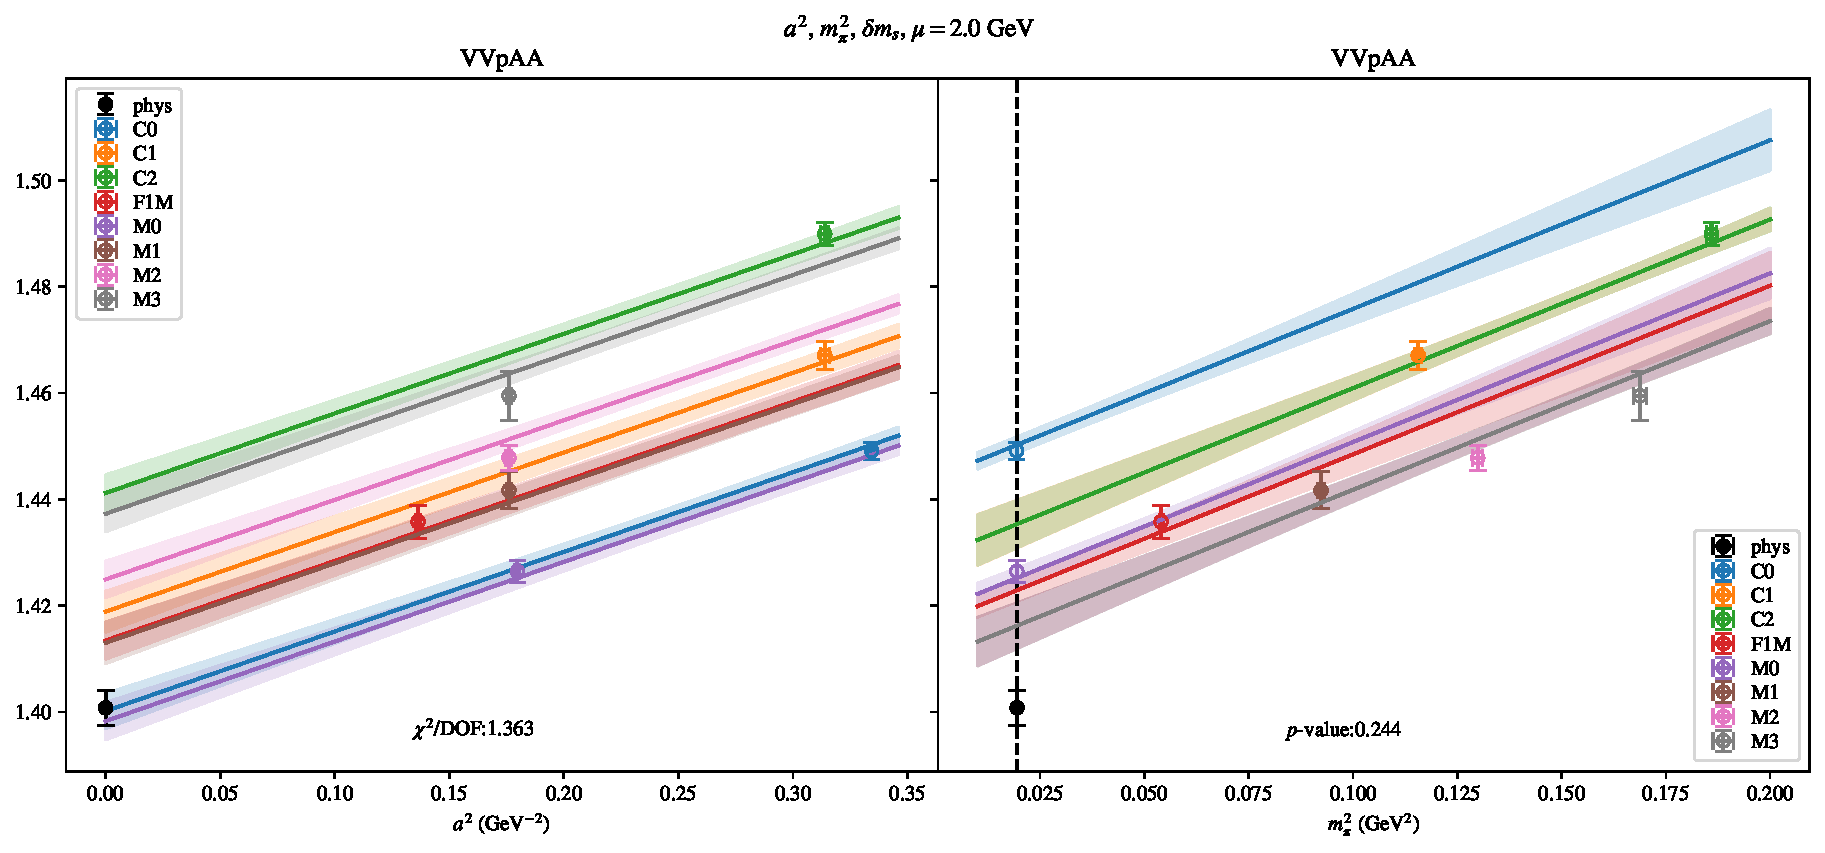
\includepdf[link, pages=-]{VVpAA/NPR/bag_a2m2delm_20.pdf}
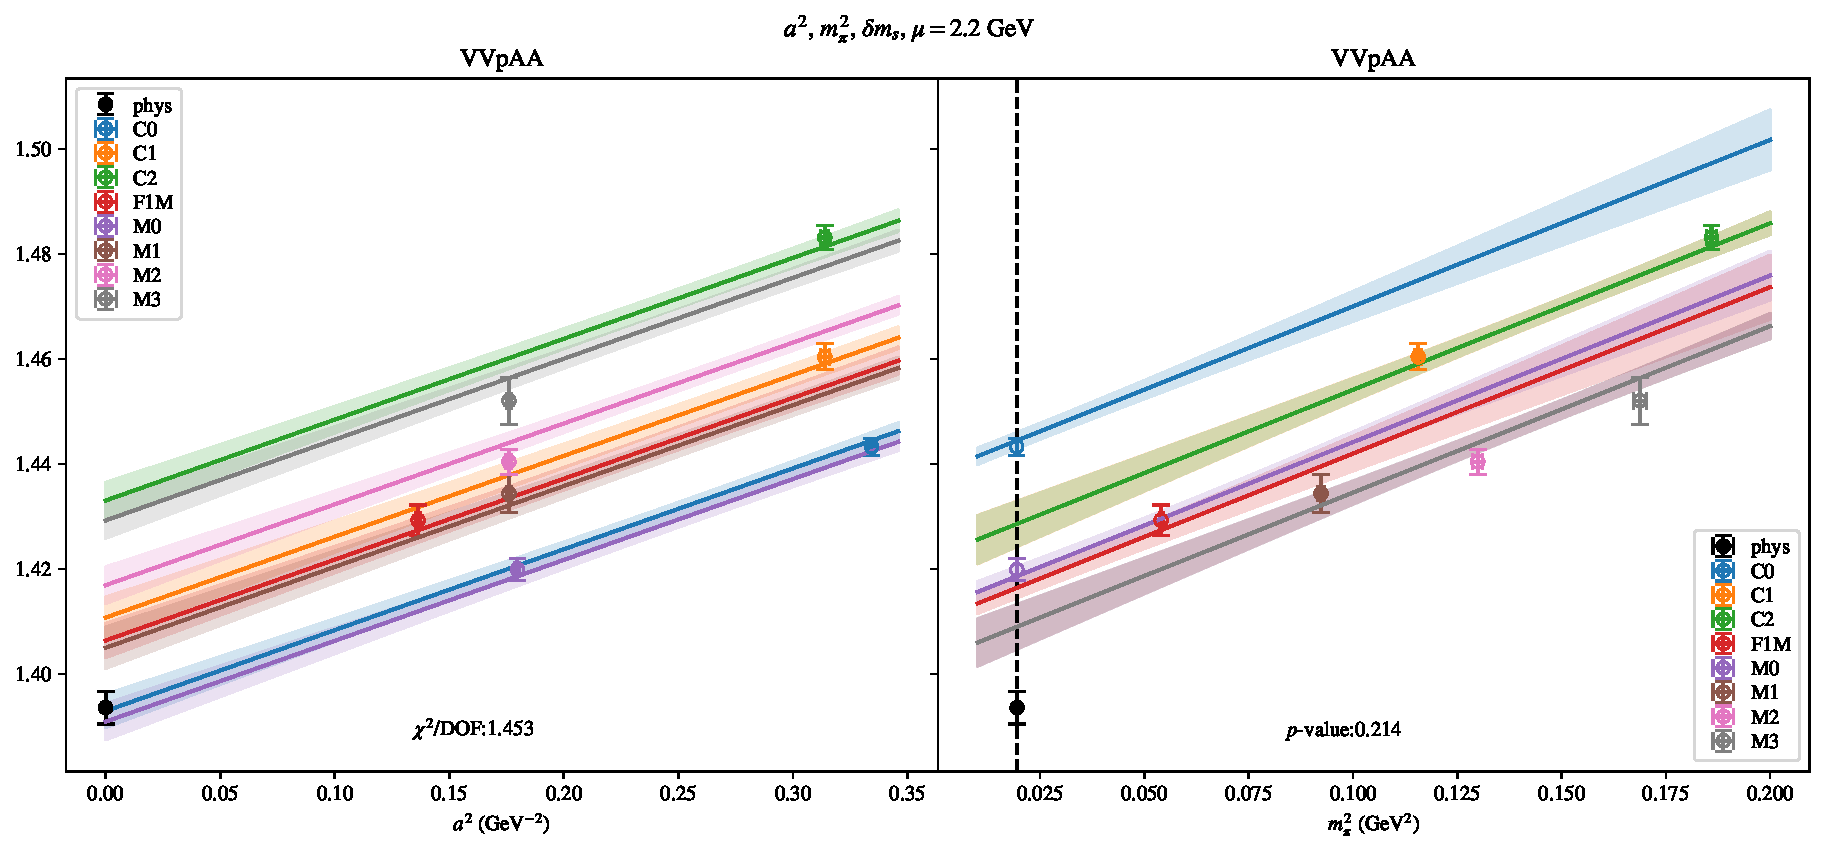
\includepdf[link, pages=-]{VVpAA/NPR/bag_a2m2delm_22.pdf}
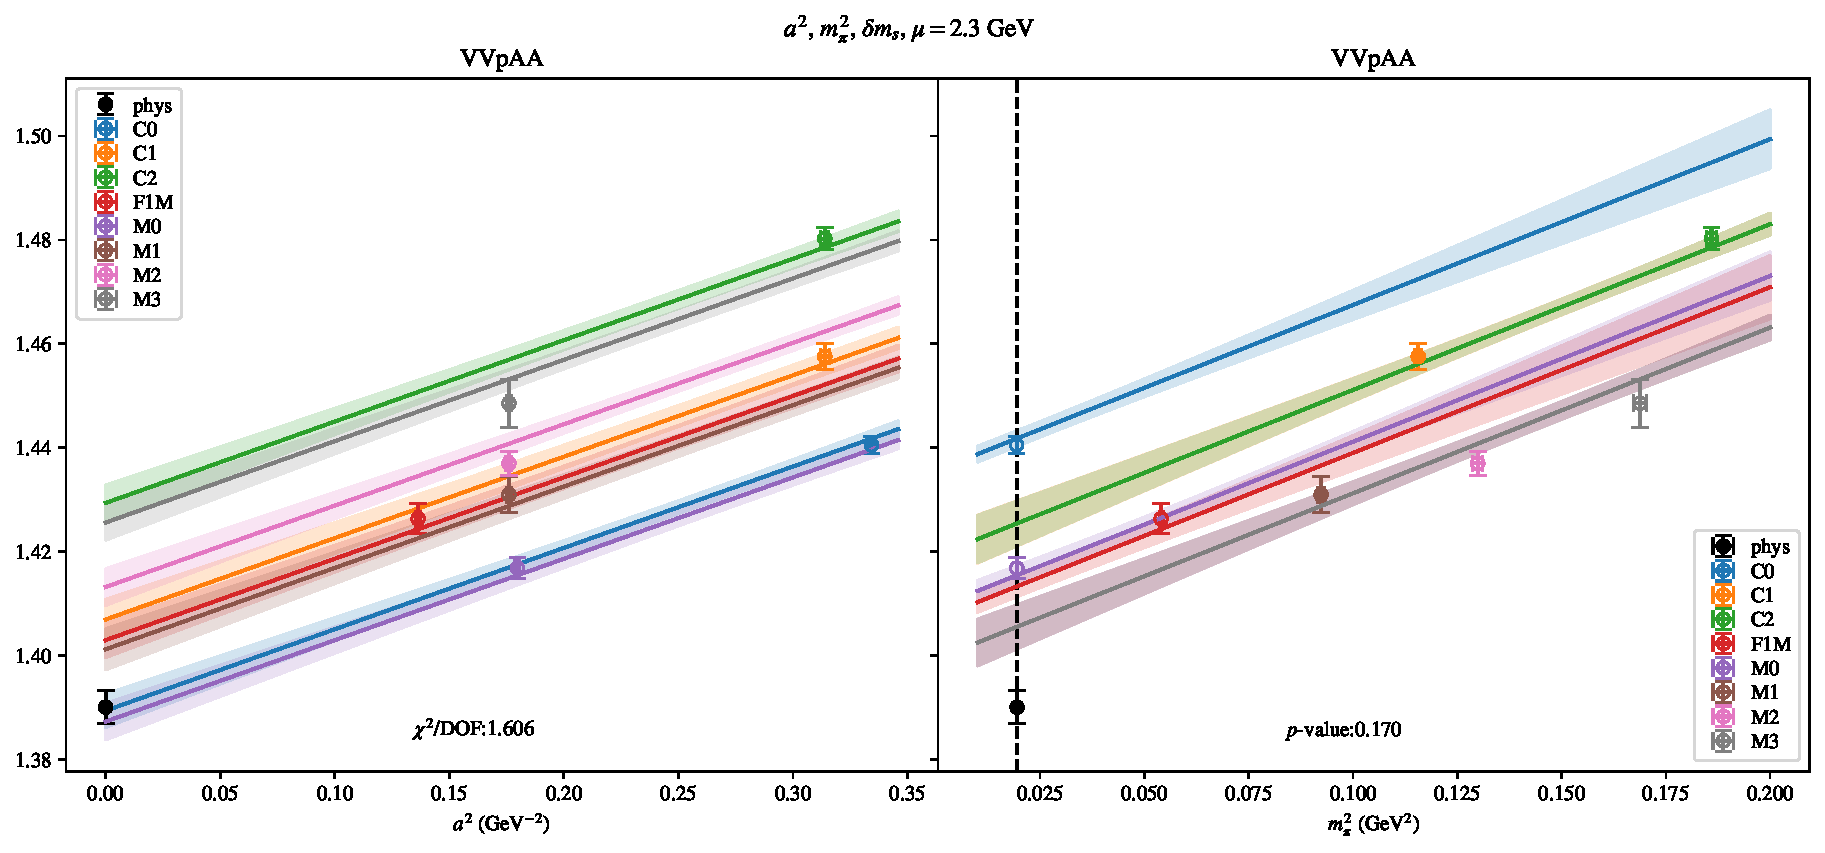
\includepdf[link, pages=-]{VVpAA/NPR/bag_a2m2delm_23.pdf}
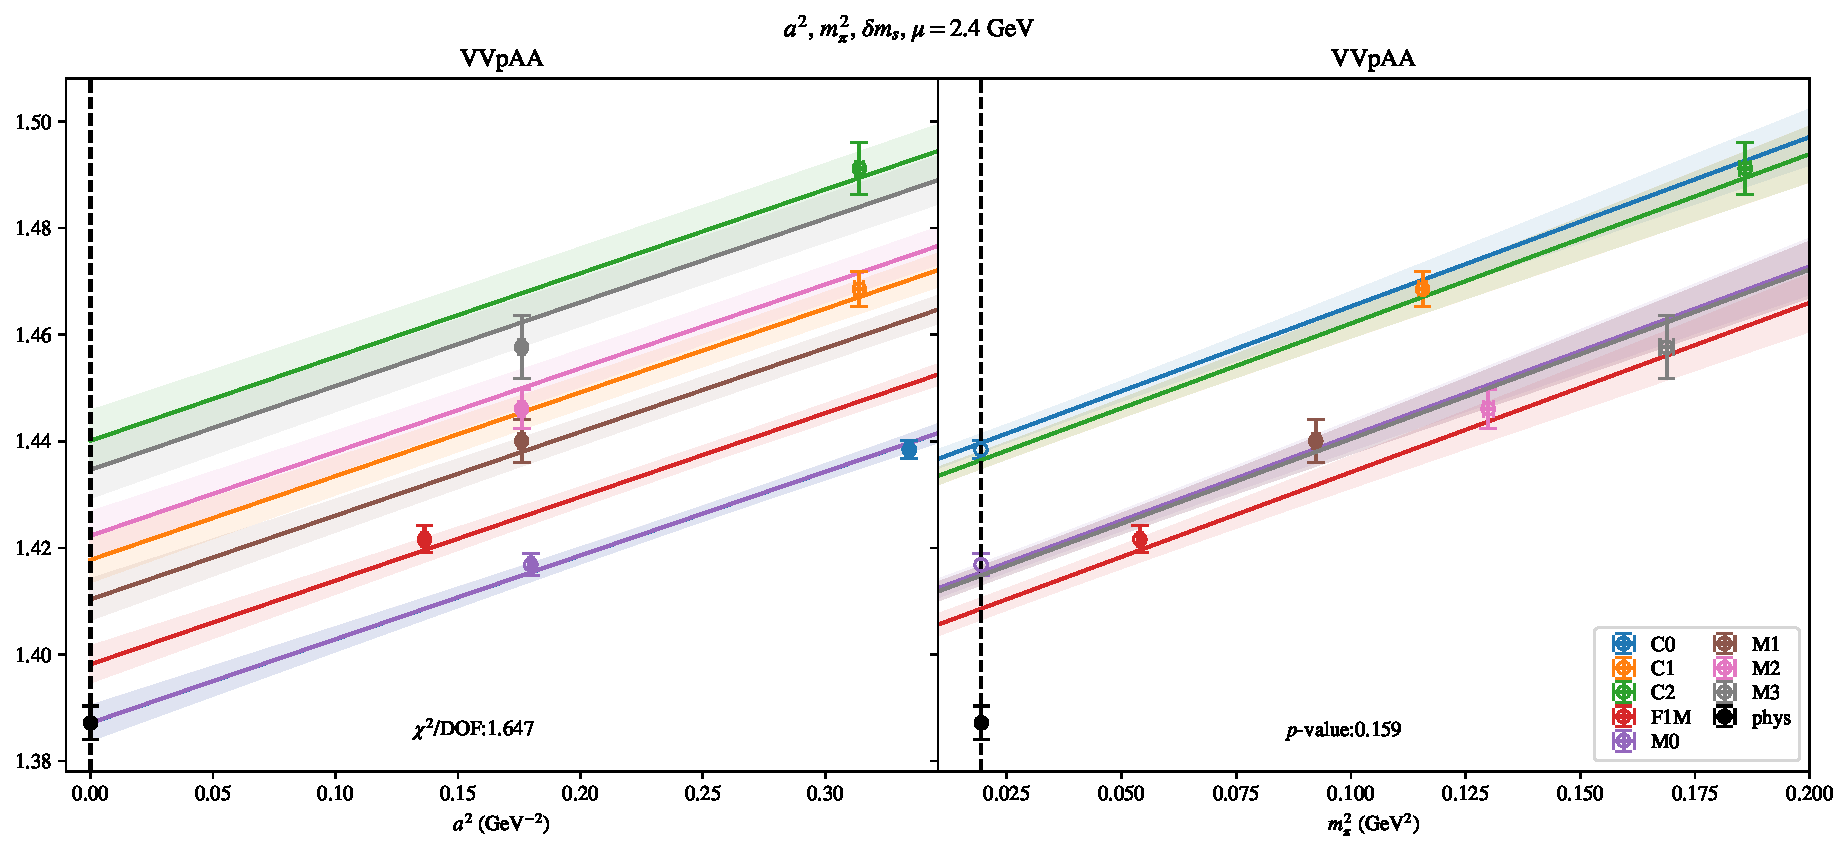
\includepdf[link, pages=-]{VVpAA/NPR/bag_a2m2delm_24.pdf}
\clearpage
\section{$\mathcal{B}_2$}
\begin{table}[h!]
\begin{center}
\begin{tabular}{|c|c|c|c|c|c|}
\hline
$\mu$ (GeV) & $a^2$, $m_\pi^2$& $a^2$, $m_\pi^2$ (no C)& $a^2$, $m_\pi^2$, $a^4$& $a^2$, $m_\pi^2$ (no M3, C2)& $a^2$, $m_\pi^2$, $\delta m_s$\\
\hline
2.0& \hyperlink{VVmAA/NPR/bag_a2m2_20.pdf.1}{\textbf{-0.984(13)}: 0.153 (0.979)} & \hyperlink{VVmAA/NPR/bag_a2m2noC_20.pdf.1}{\textbf{-0.939(53)}: 0.002 (0.998)} & \hyperlink{VVmAA/NPR/bag_a2a4m2_20.pdf.1}{\textbf{-0.916(89)}: 0.045 (0.996)} & \hyperlink{VVmAA/NPR/bag_a2m2mcut_20.pdf.1}{\textbf{-0.984(14)}: 0.229 (0.876)} & \hyperlink{VVmAA/NPR/bag_a2m2delm_20.pdf.1}{\textbf{-0.985(13)}: 0.091 (0.985)}\\
2.2& \hyperlink{VVmAA/NPR/bag_a2m2_22.pdf.1}{\textbf{-0.999(12)}: 0.148 (0.981)} & \hyperlink{VVmAA/NPR/bag_a2m2noC_22.pdf.1}{\textbf{-0.961(47)}: 0.008 (0.992)} & \hyperlink{VVmAA/NPR/bag_a2a4m2_22.pdf.1}{\textbf{-0.937(80)}: 0.032 (0.998)} & \hyperlink{VVmAA/NPR/bag_a2m2mcut_22.pdf.1}{\textbf{-1.000(13)}: 0.224 (0.88)} & \hyperlink{VVmAA/NPR/bag_a2m2delm_22.pdf.1}{\textbf{-1.000(12)}: 0.108 (0.98)}\\
2.3& \hyperlink{VVmAA/NPR/bag_a2m2_23.pdf.1}{\textbf{-1.006(11)}: 0.18 (0.97)} & \hyperlink{VVmAA/NPR/bag_a2m2noC_23.pdf.1}{\textbf{-0.967(42)}: 0.008 (0.992)} & \hyperlink{VVmAA/NPR/bag_a2a4m2_23.pdf.1}{\textbf{-0.940(72)}: 0.02 (0.999)} & \hyperlink{VVmAA/NPR/bag_a2m2mcut_23.pdf.1}{\textbf{-1.006(11)}: 0.282 (0.839)} & \hyperlink{VVmAA/NPR/bag_a2m2delm_23.pdf.1}{\textbf{-1.006(11)}: 0.104 (0.981)}\\
2.4& \hyperlink{VVmAA/NPR/bag_a2m2_24.pdf.1}{\textbf{-1.0100(98)}: 0.198 (0.963)} & \hyperlink{VVmAA/NPR/bag_a2m2noC_24.pdf.1}{\textbf{-0.974(39)}: 0.009 (0.991)} & \hyperlink{VVmAA/NPR/bag_a2a4m2_24.pdf.1}{\textbf{-0.949(66)}: 0.027 (0.999)} & \hyperlink{VVmAA/NPR/bag_a2m2mcut_24.pdf.1}{\textbf{-1.010(10)}: 0.313 (0.816)} & \hyperlink{VVmAA/NPR/bag_a2m2delm_24.pdf.1}{\textbf{-1.0105(97)}: 0.121 (0.975)}\\
\hline
\end{tabular}
\caption{Physical point value from chiral and continuum extrapolation at renormalisation scale $\mu$. Entries are \textbf{value(error)}: $\chi^2/\text{DOF}$ ($p$-value).}
\end{center}
\end{table}
\begin{table}[h!]
\begin{center}
\begin{tabular}{|c c|c|c|c|c|c|}
\hline
$\mu$ (GeV) &  & $a^2$, $m_\pi^2$& $a^2$, $m_\pi^2$ (no C)& $a^2$, $m_\pi^2$, $a^4$& $a^2$, $m_\pi^2$ (no M3, C2)& $a^2$, $m_\pi^2$, $\delta m_s$\\
\hline
\multirow{3}{0.5in}{2.0} & $\alpha$ & 0.150(46)& -0.12(31)& -0.48(82)& 0.150(50)& 0.157(46)\\
 & $\beta$ & -0.0020(13)& -0.0024(24)& -0.0017(13)& -0.0017(23)& -0.0006(24)\\
 & $\gamma$ &  &  & 1.3(16)&  & -0.055(80)\\
\hline
\multirow{3}{0.5in}{2.2} & $\alpha$ & 0.204(40)& -0.03(28)& -0.37(74)& 0.205(43)& 0.208(40)\\
 & $\beta$ & -0.0017(10)& -0.0016(19)& -0.0013(11)& -0.0013(18)& -0.0006(20)\\
 & $\gamma$ &  &  & 1.2(15)&  & -0.041(68)\\
\hline
\multirow{3}{0.5in}{2.3} & $\alpha$ & 0.229(37)& -0.004(246)& -0.38(65)& 0.230(39)& 0.232(37)\\
 & $\beta$ & -0.00180(98)& -0.0017(17)& -0.0015(10)& -0.0015(16)& -0.0006(19)\\
 & $\gamma$ &  &  & 1.2(13)&  & -0.047(63)\\
\hline
\multirow{3}{0.5in}{2.4} & $\alpha$ & 0.249(33)& 0.03(23)& -0.32(61)& 0.250(35)& 0.253(33)\\
 & $\beta$ & -0.00181(87)& -0.0017(14)& -0.00150(93)& -0.0016(15)& -0.0007(17)\\
 & $\gamma$ &  &  & 1.2(12)&  & -0.043(57)\\
\hline
\end{tabular}
\caption{Fit values of coefficients in $Q = Q_{phys} + \mathbf{\alpha} a^2 + \mathbf{\beta}\left(\frac{m_\pi^2}{f_\pi^2}-\frac{m_{\pi,PDG}^2}{f_\pi^2}\right) + \gamma(\ldots)$}
\end{center}
\end{table}
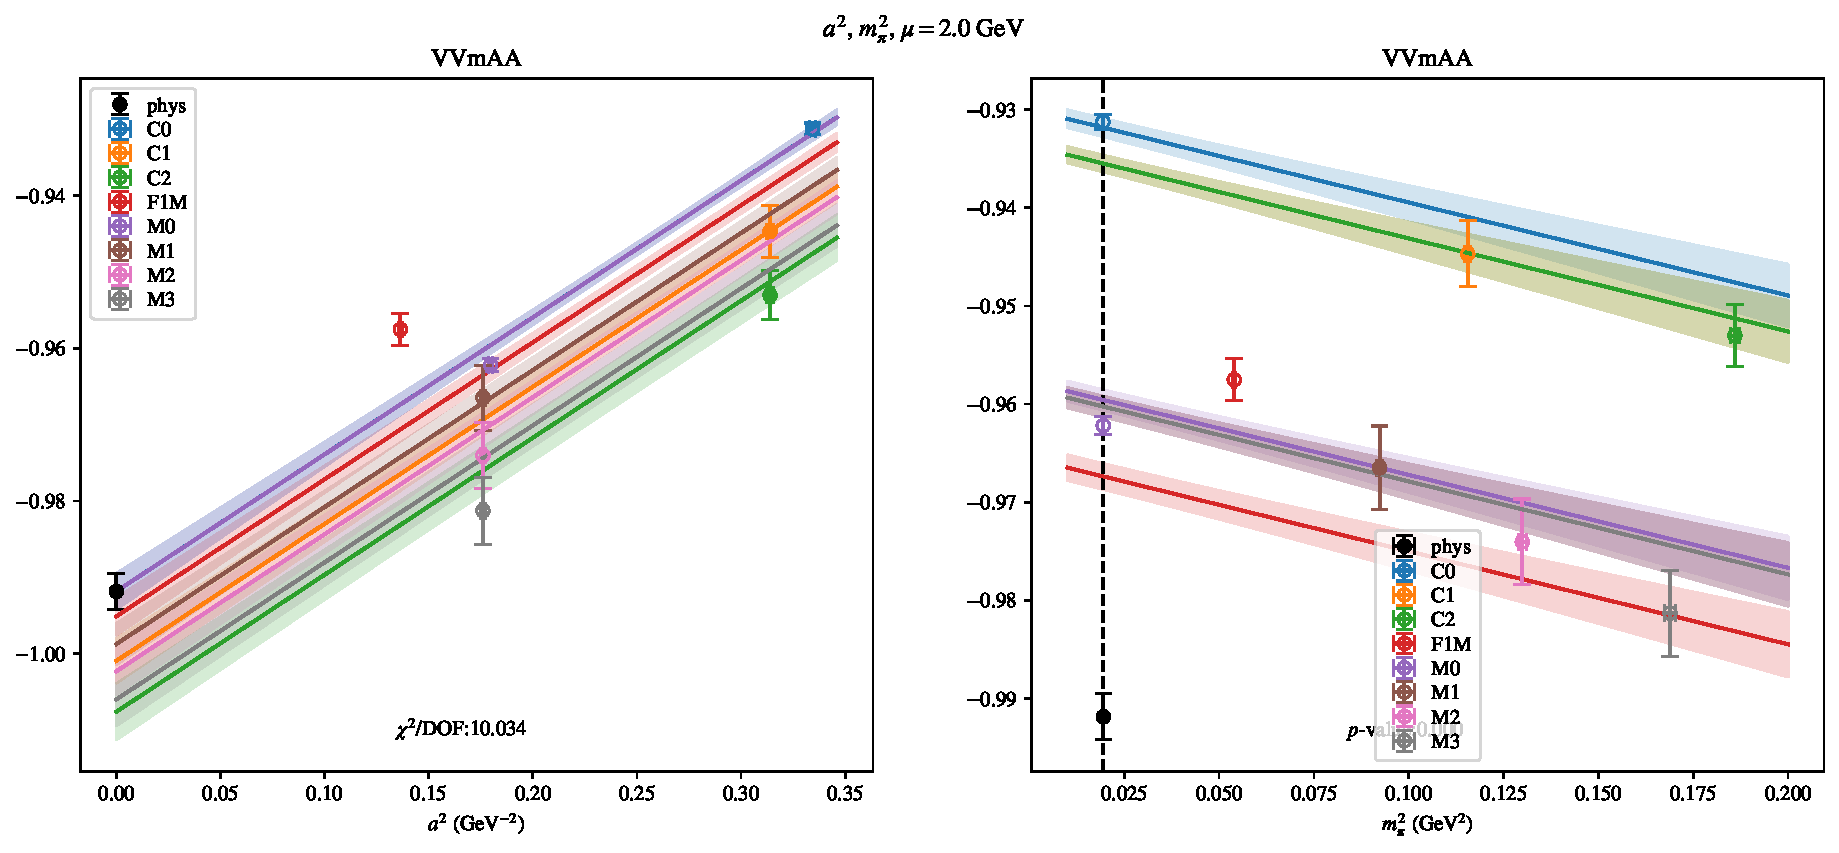
\includepdf[link, pages=-]{VVmAA/NPR/bag_a2m2_20.pdf}
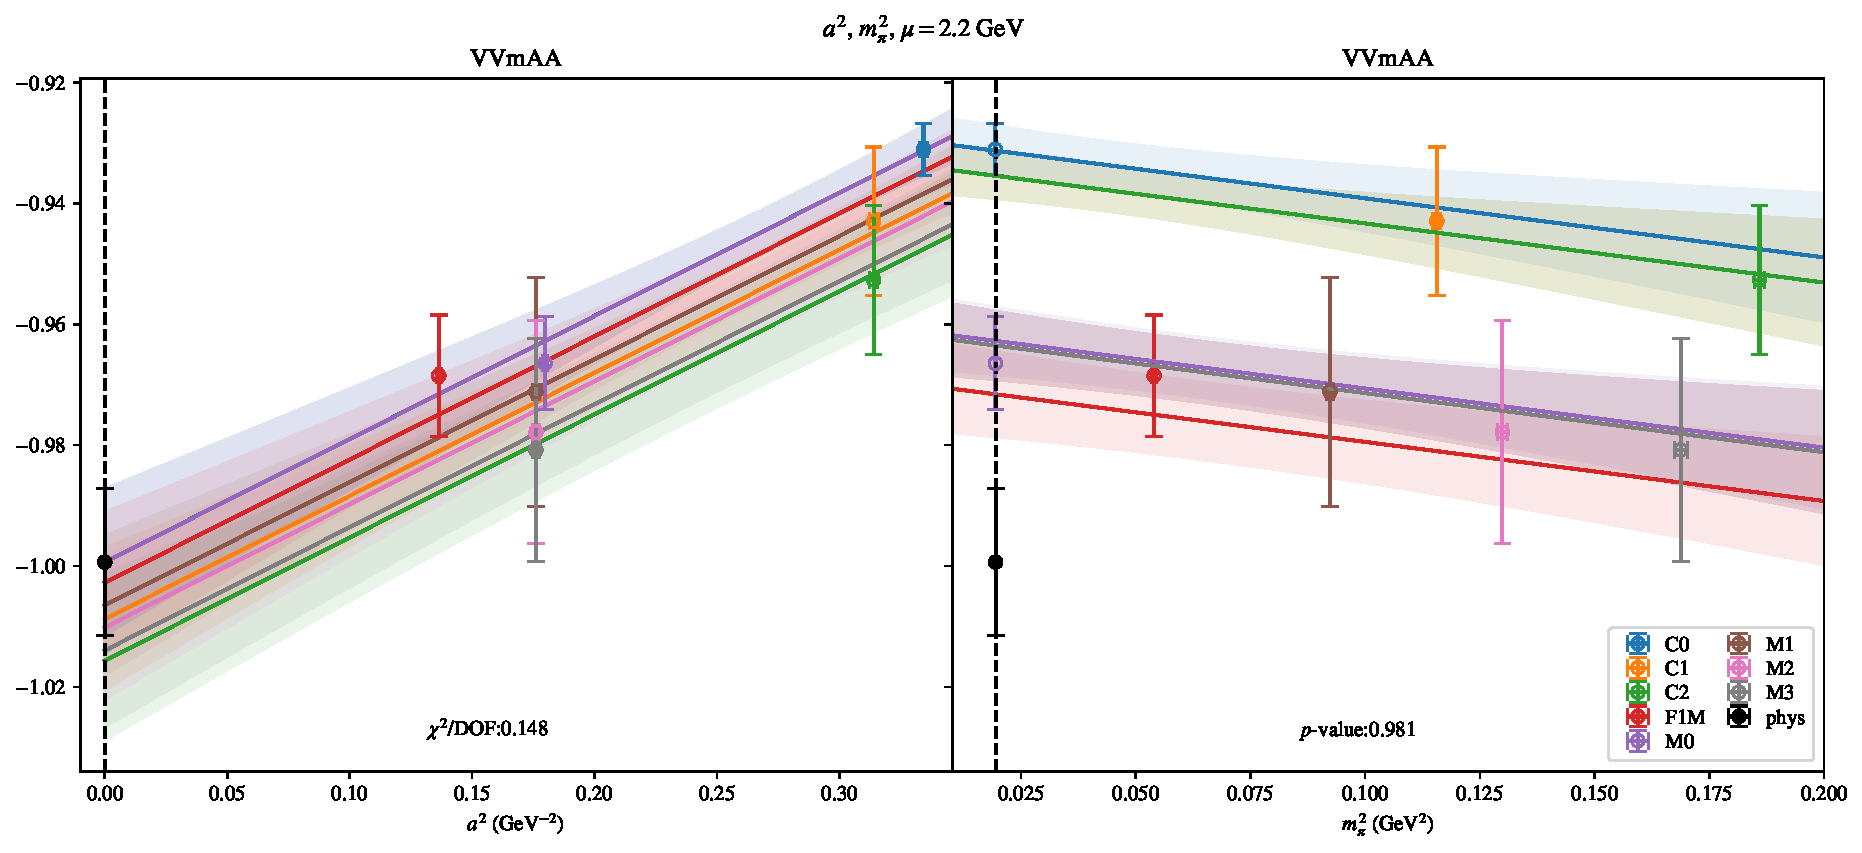
\includepdf[link, pages=-]{VVmAA/NPR/bag_a2m2_22.pdf}
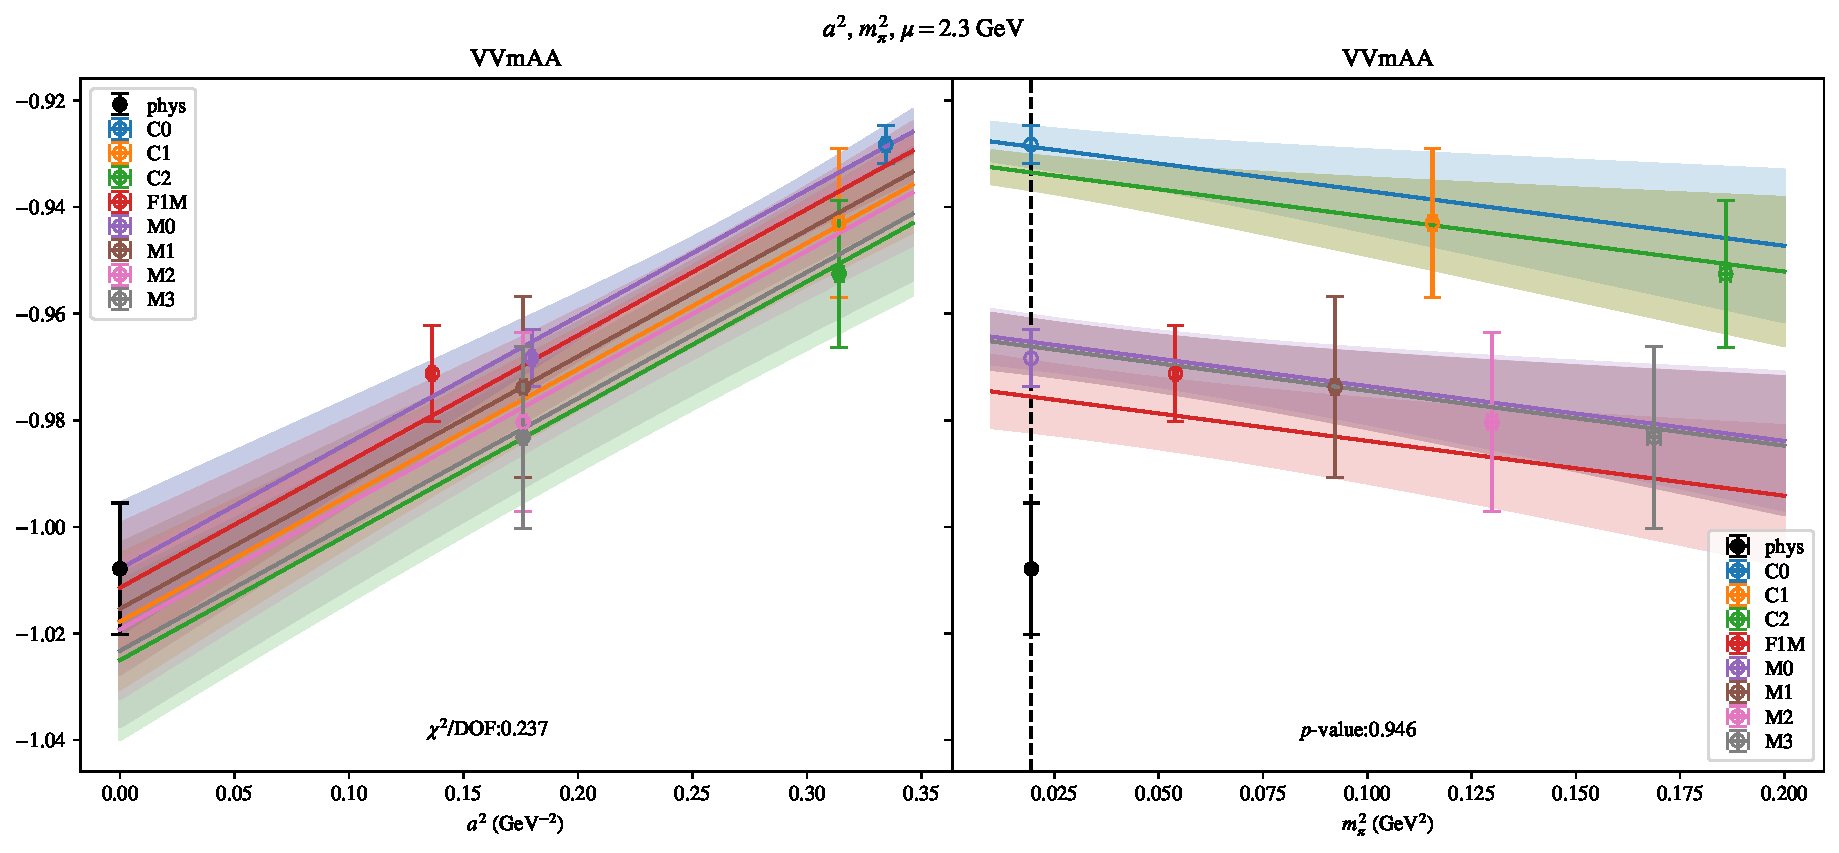
\includepdf[link, pages=-]{VVmAA/NPR/bag_a2m2_23.pdf}
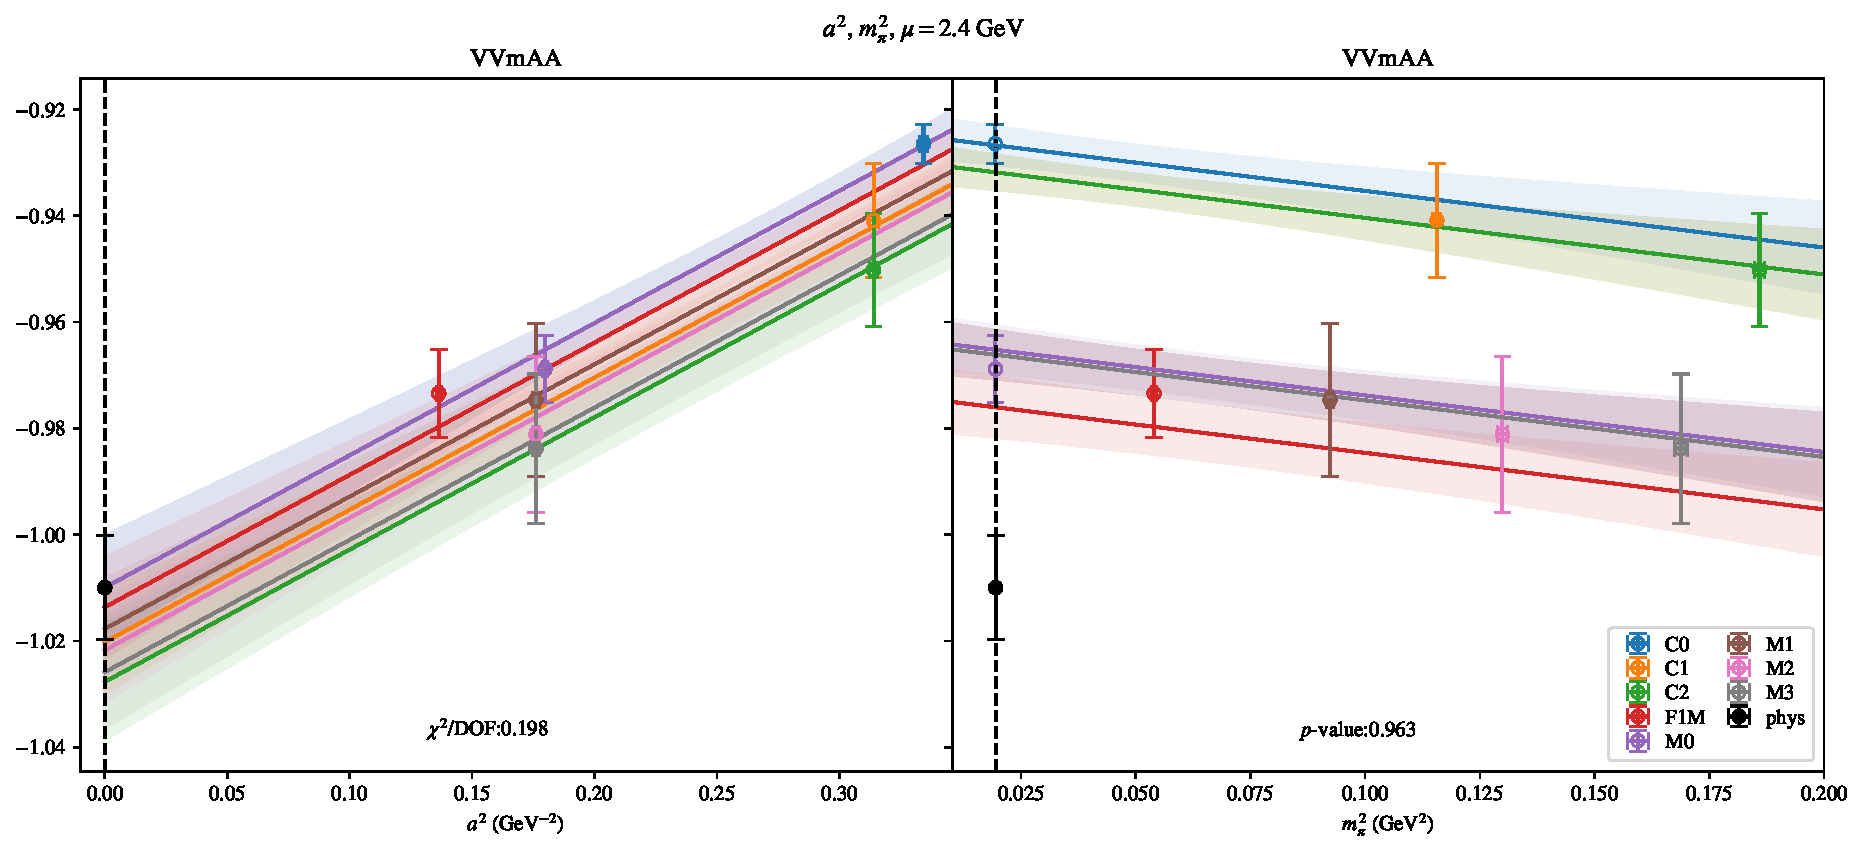
\includepdf[link, pages=-]{VVmAA/NPR/bag_a2m2_24.pdf}
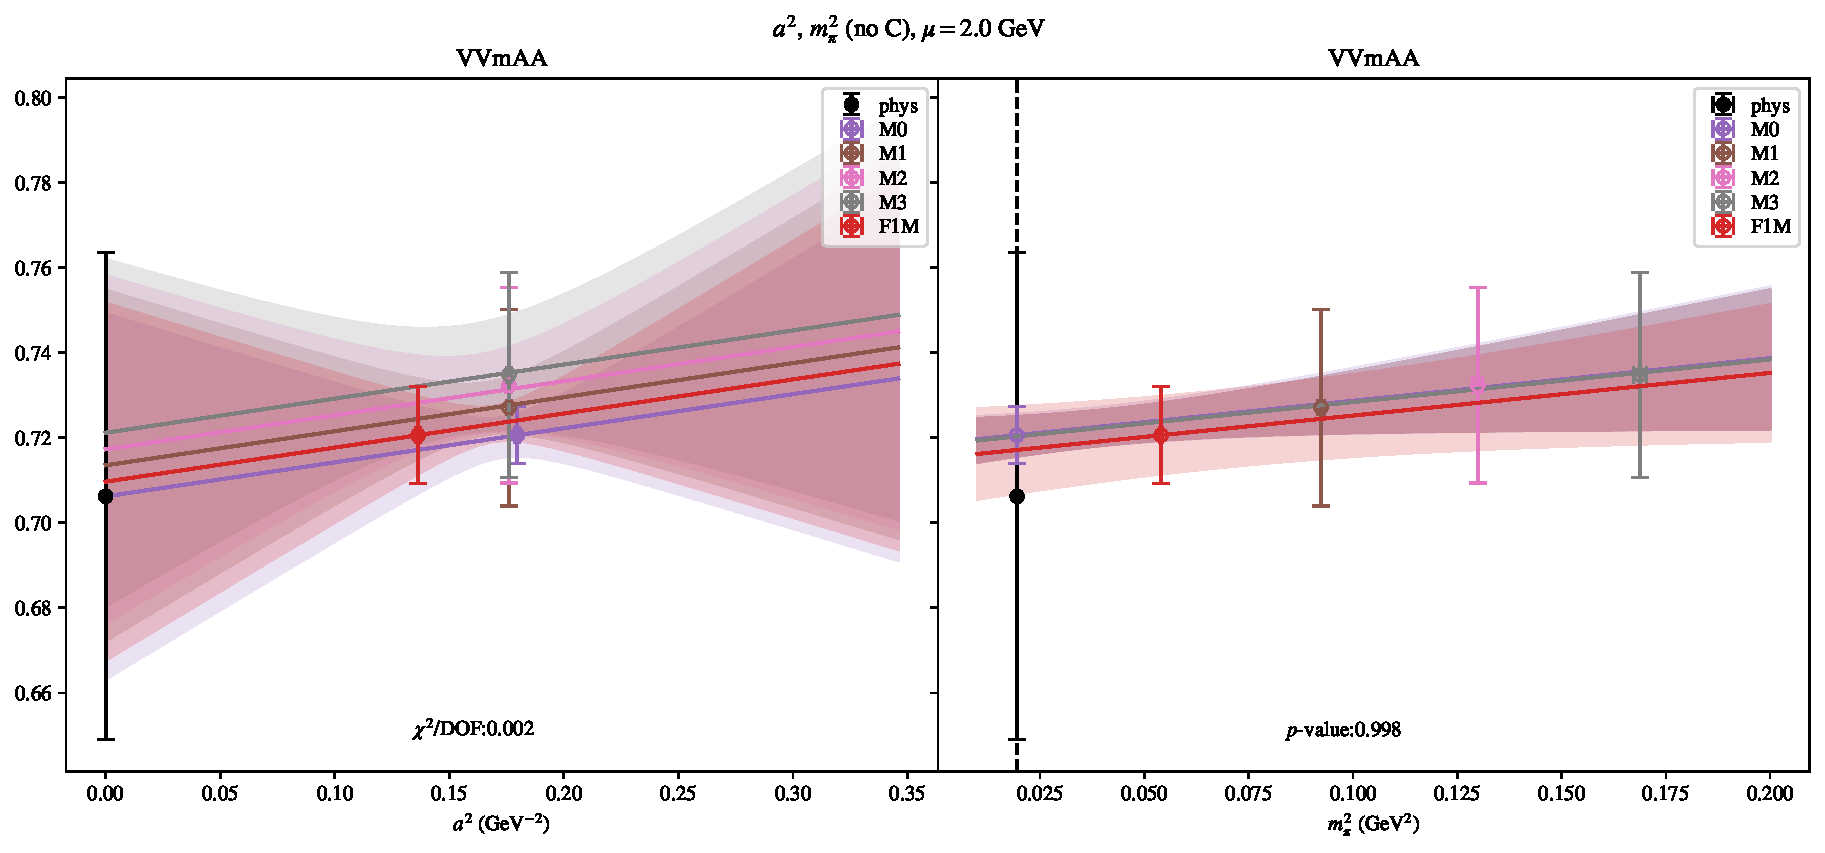
\includepdf[link, pages=-]{VVmAA/NPR/bag_a2m2noC_20.pdf}
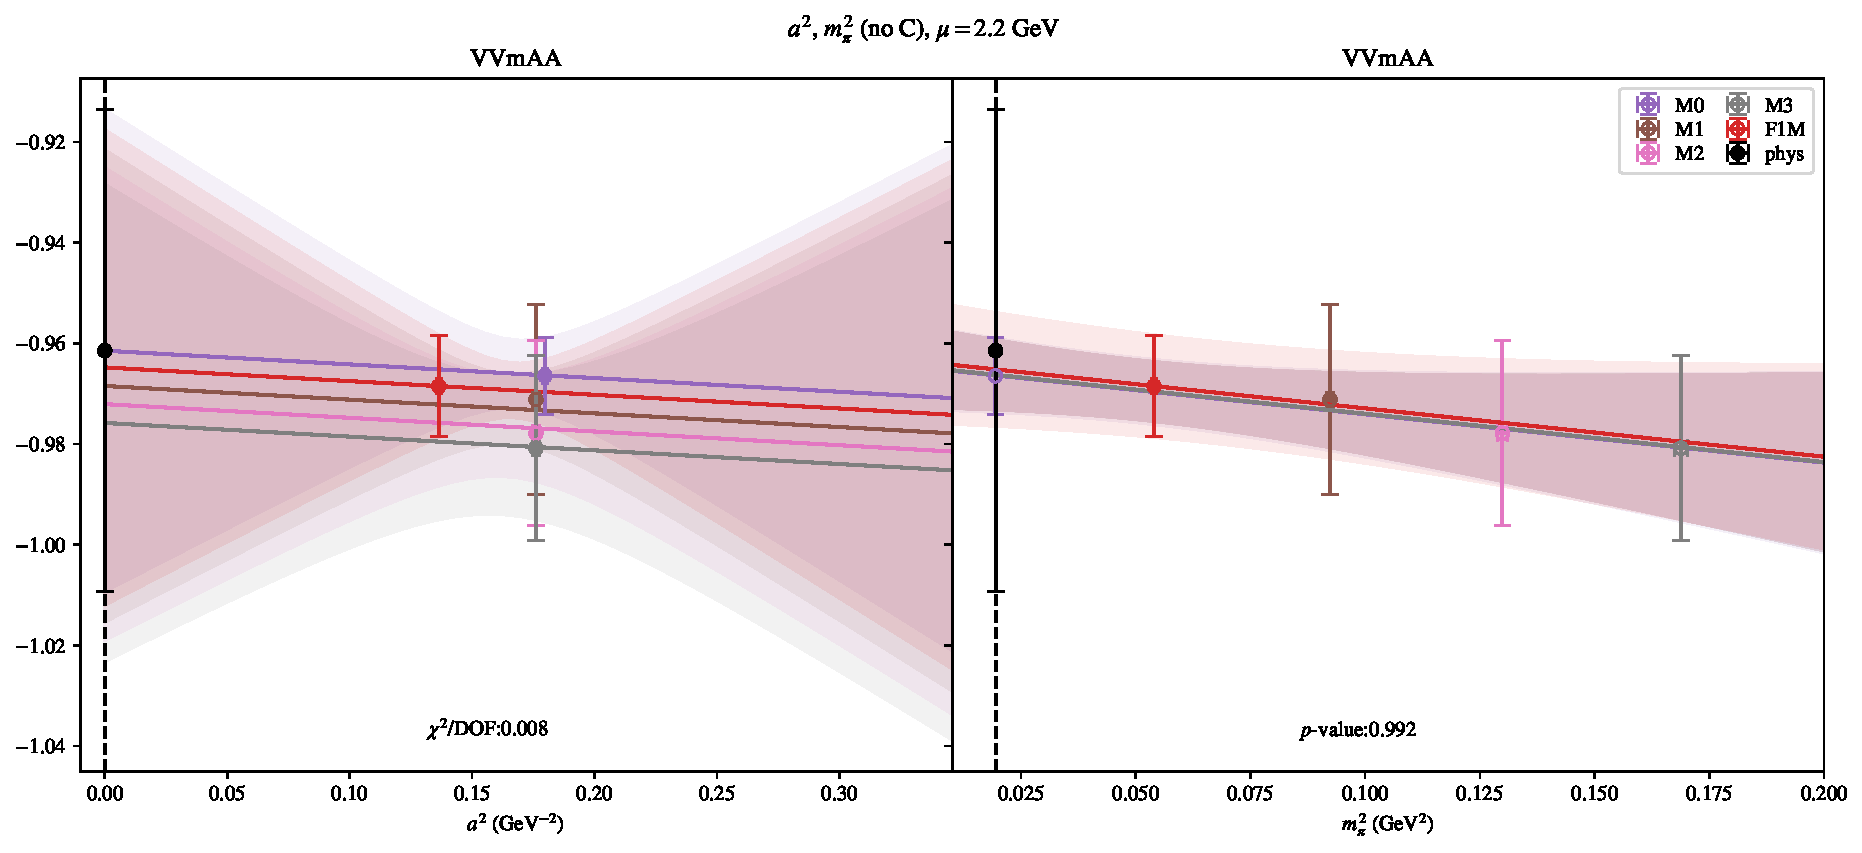
\includepdf[link, pages=-]{VVmAA/NPR/bag_a2m2noC_22.pdf}
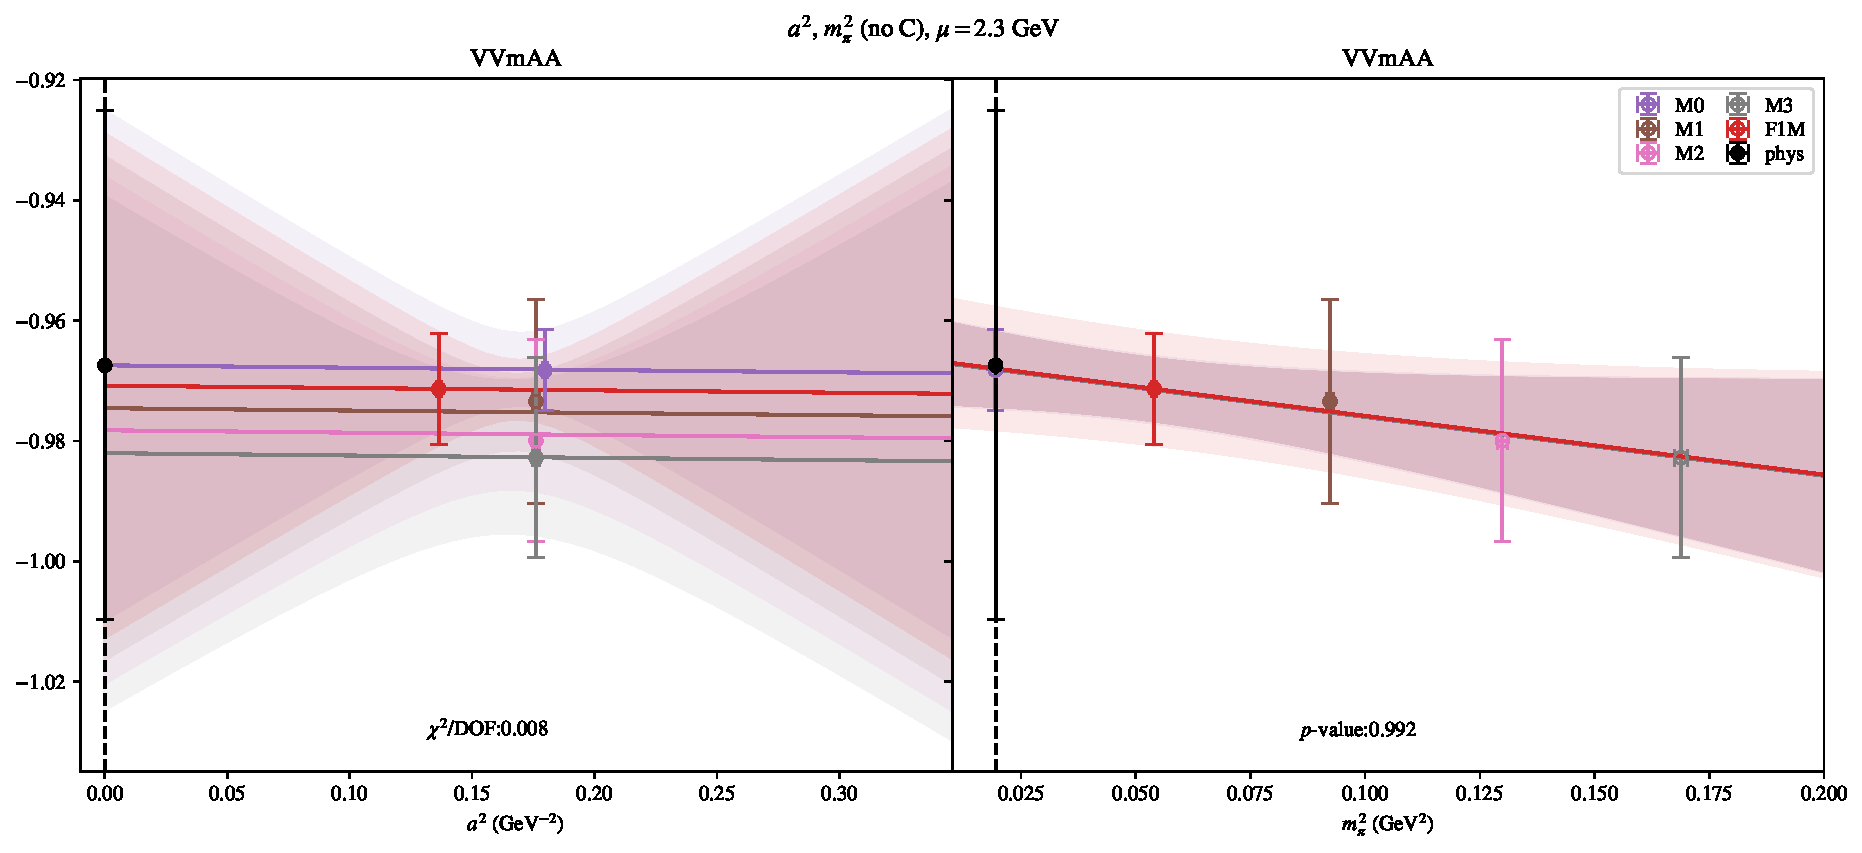
\includepdf[link, pages=-]{VVmAA/NPR/bag_a2m2noC_23.pdf}
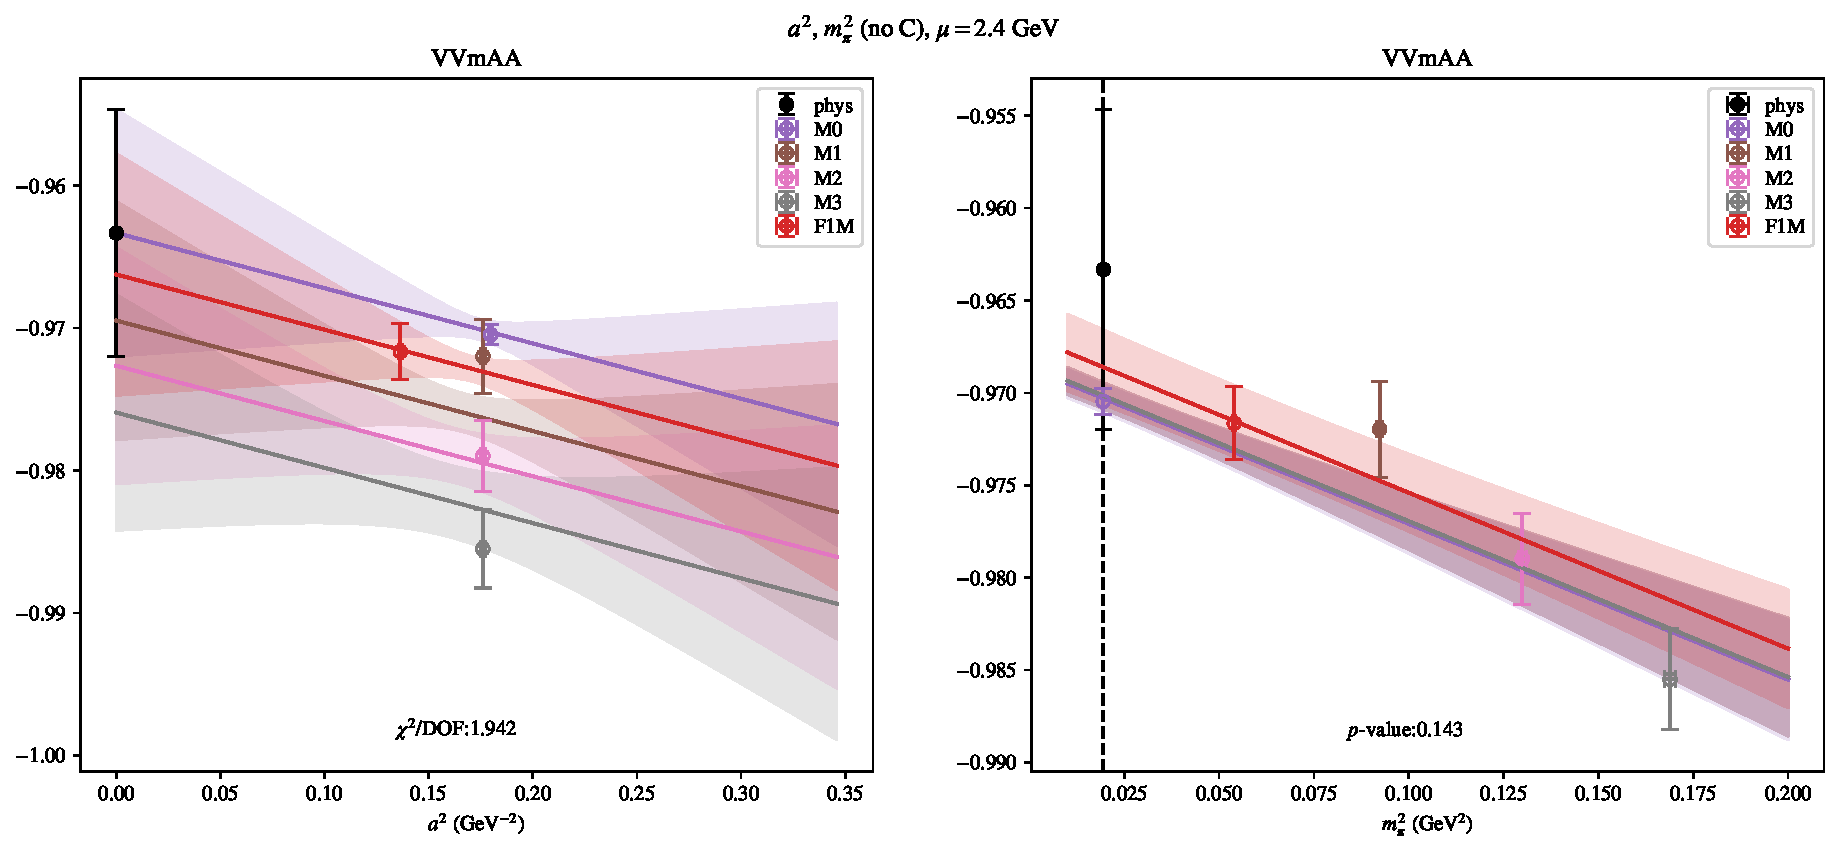
\includepdf[link, pages=-]{VVmAA/NPR/bag_a2m2noC_24.pdf}
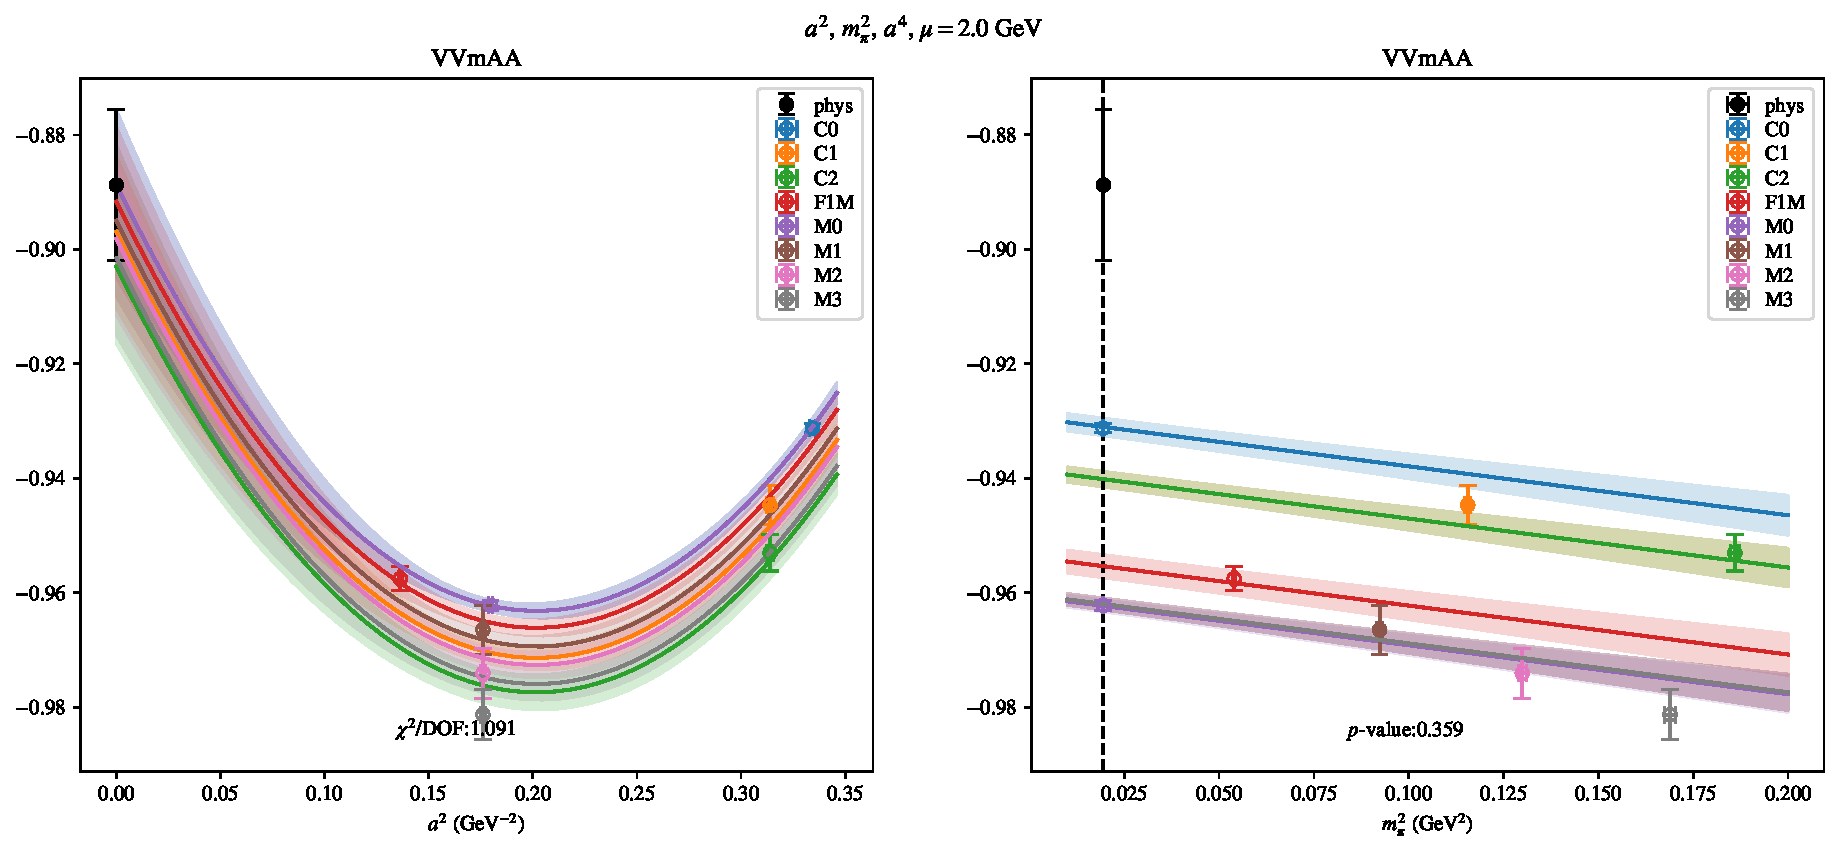
\includepdf[link, pages=-]{VVmAA/NPR/bag_a2a4m2_20.pdf}
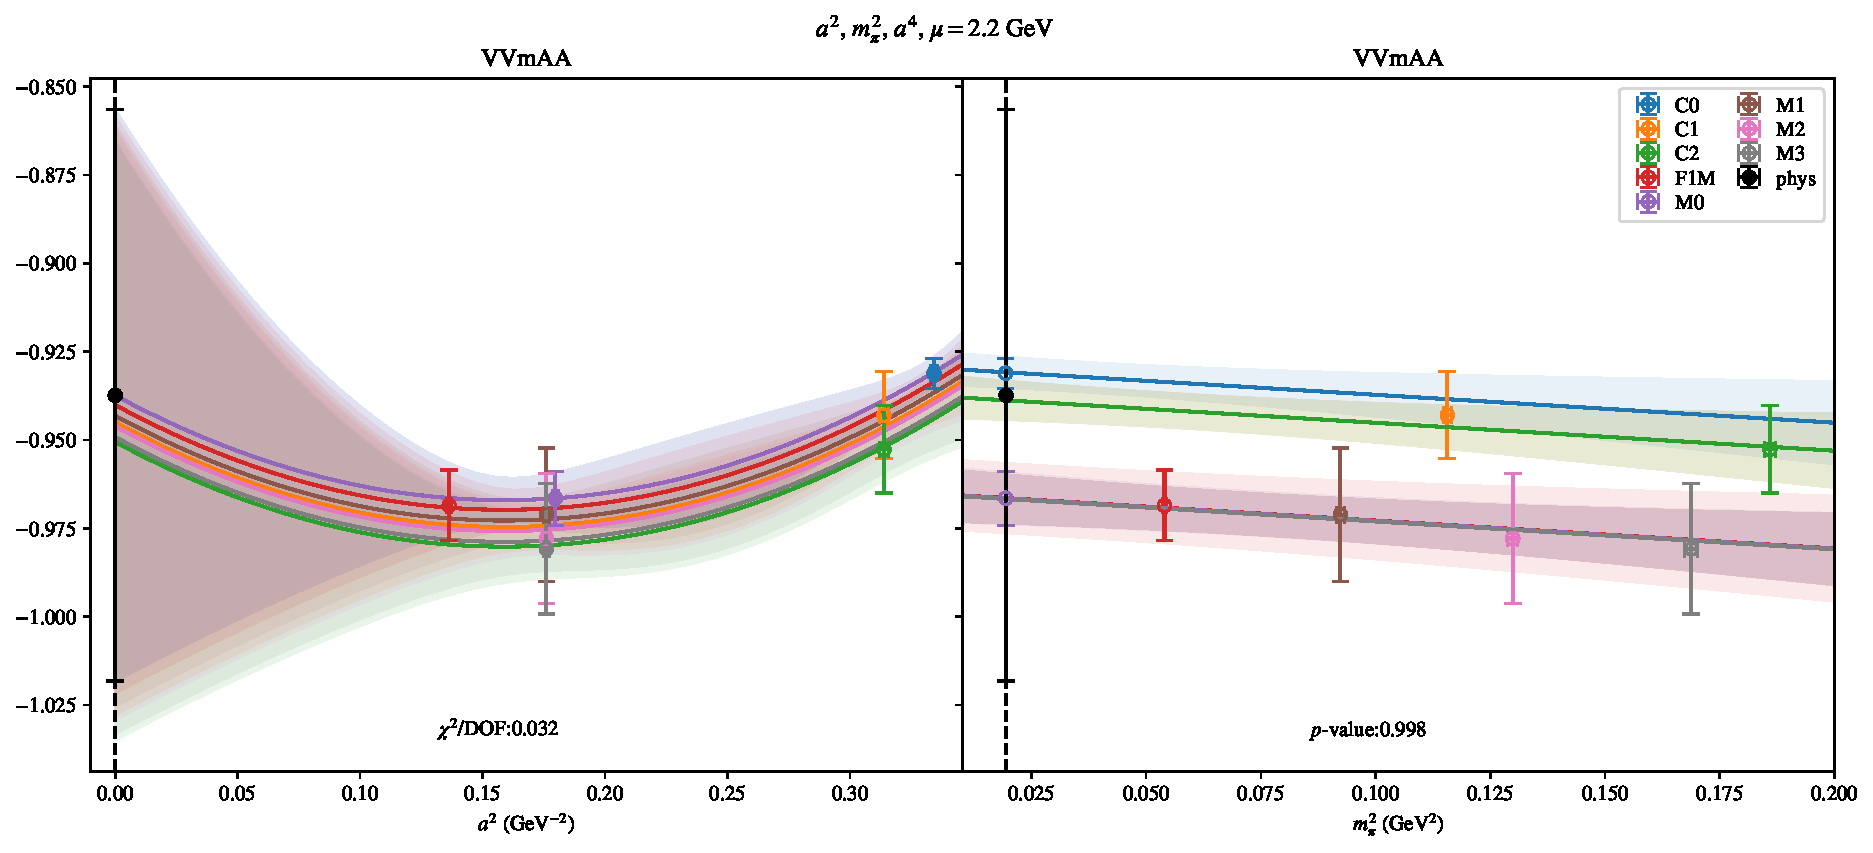
\includepdf[link, pages=-]{VVmAA/NPR/bag_a2a4m2_22.pdf}
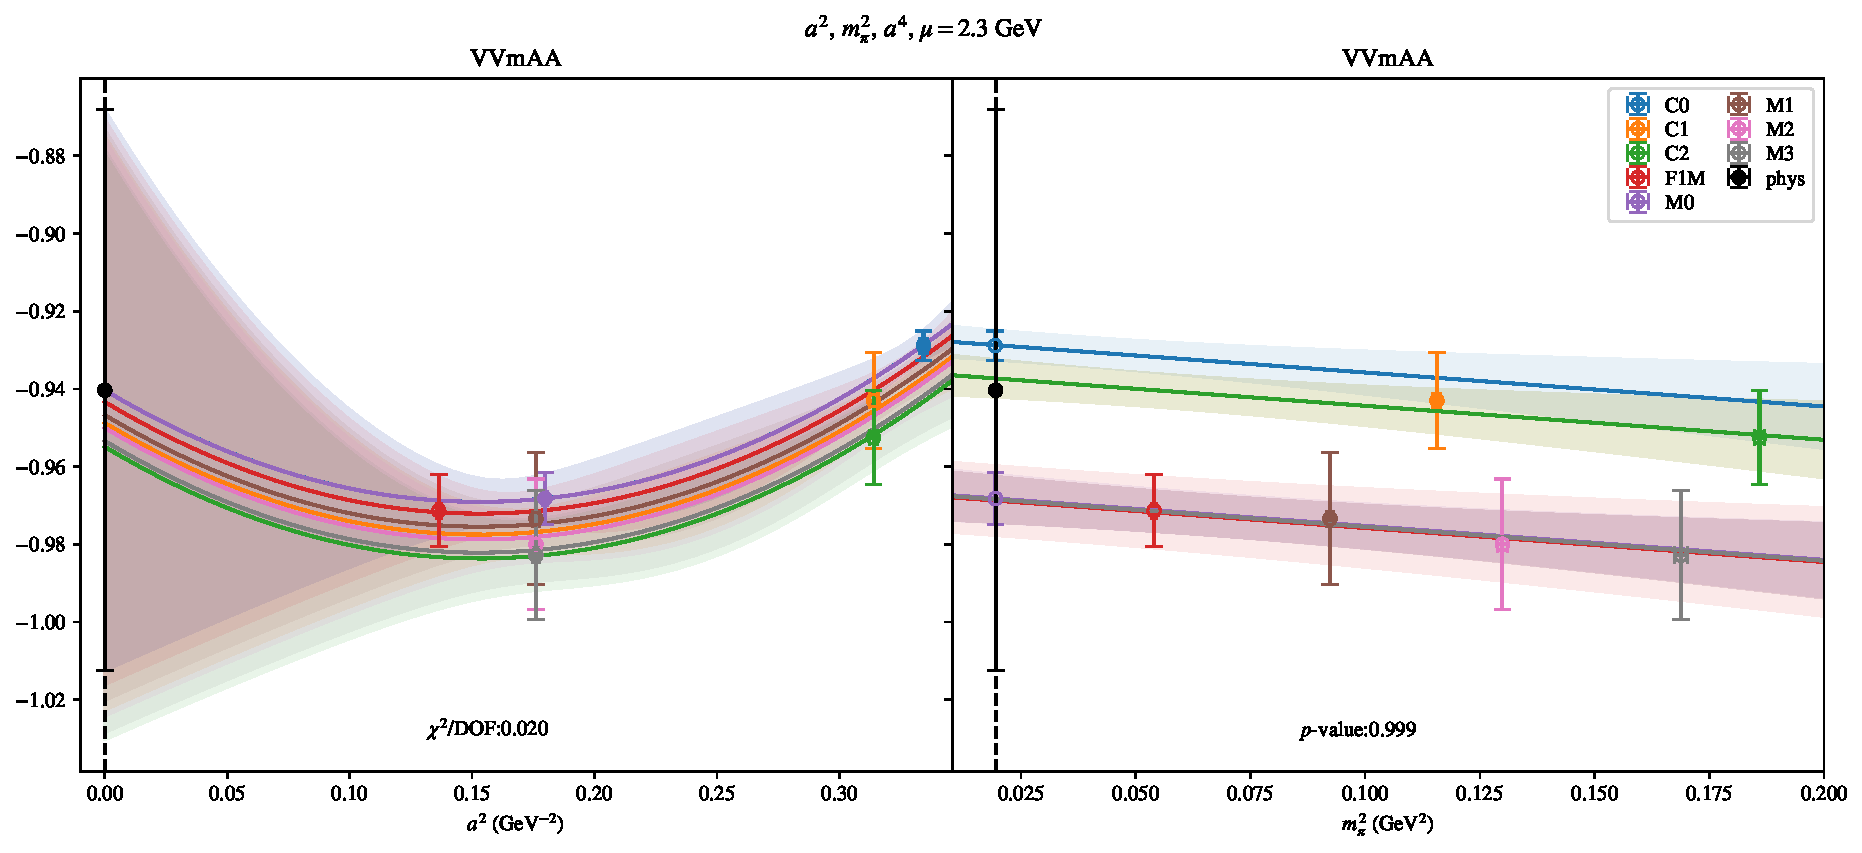
\includepdf[link, pages=-]{VVmAA/NPR/bag_a2a4m2_23.pdf}
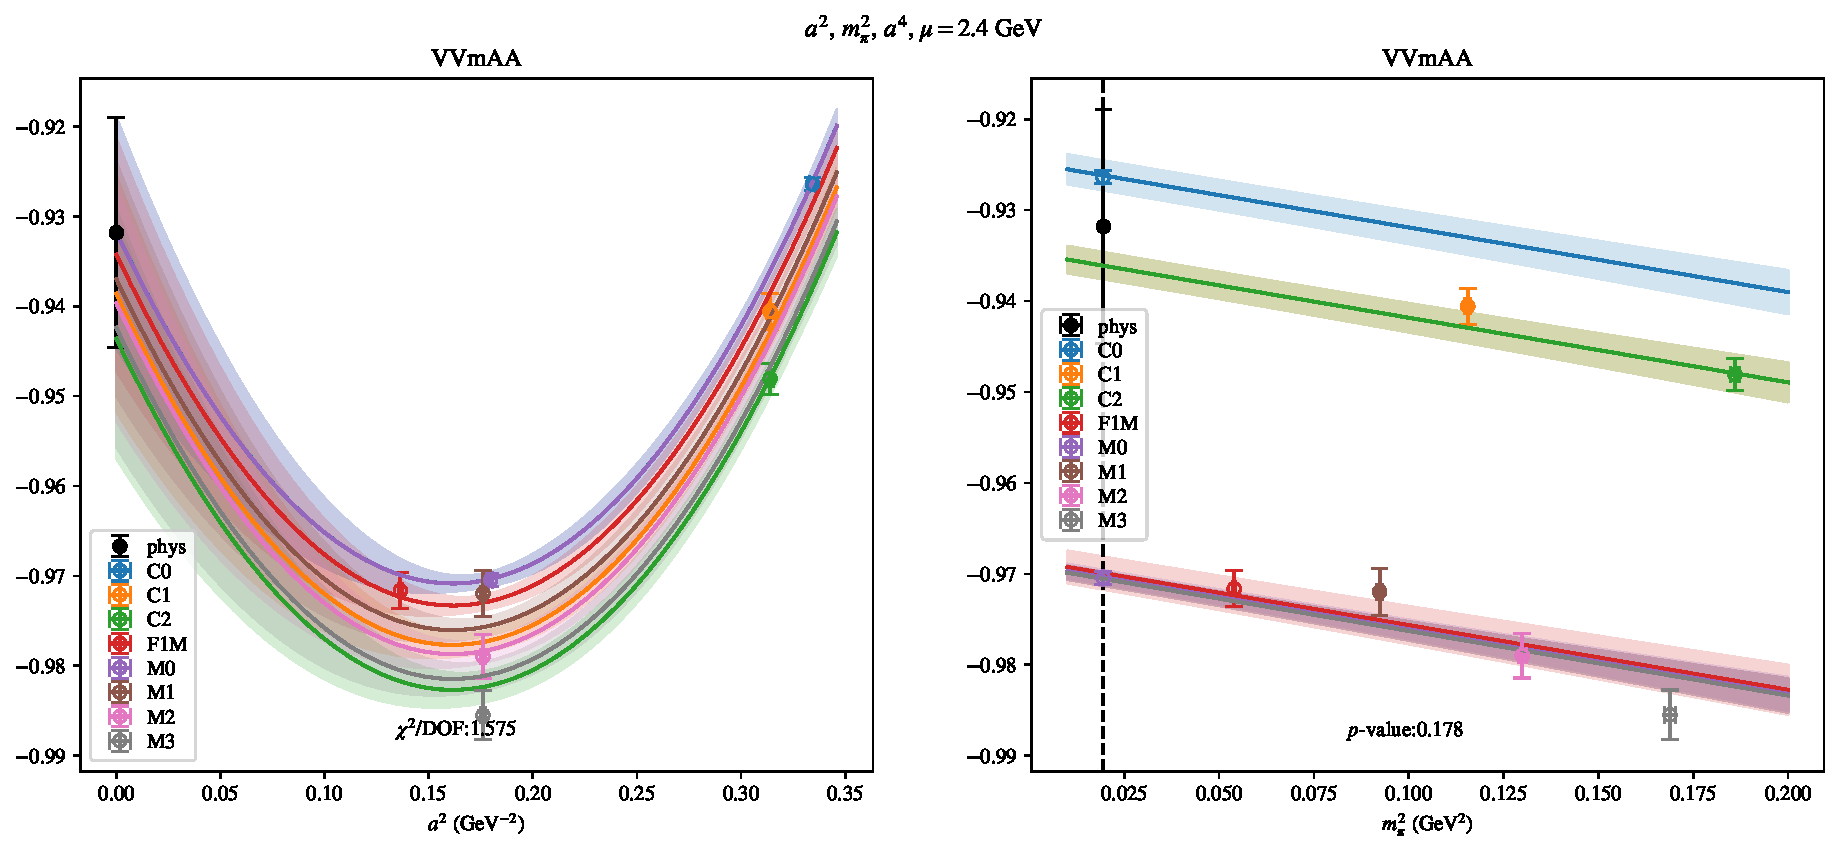
\includepdf[link, pages=-]{VVmAA/NPR/bag_a2a4m2_24.pdf}
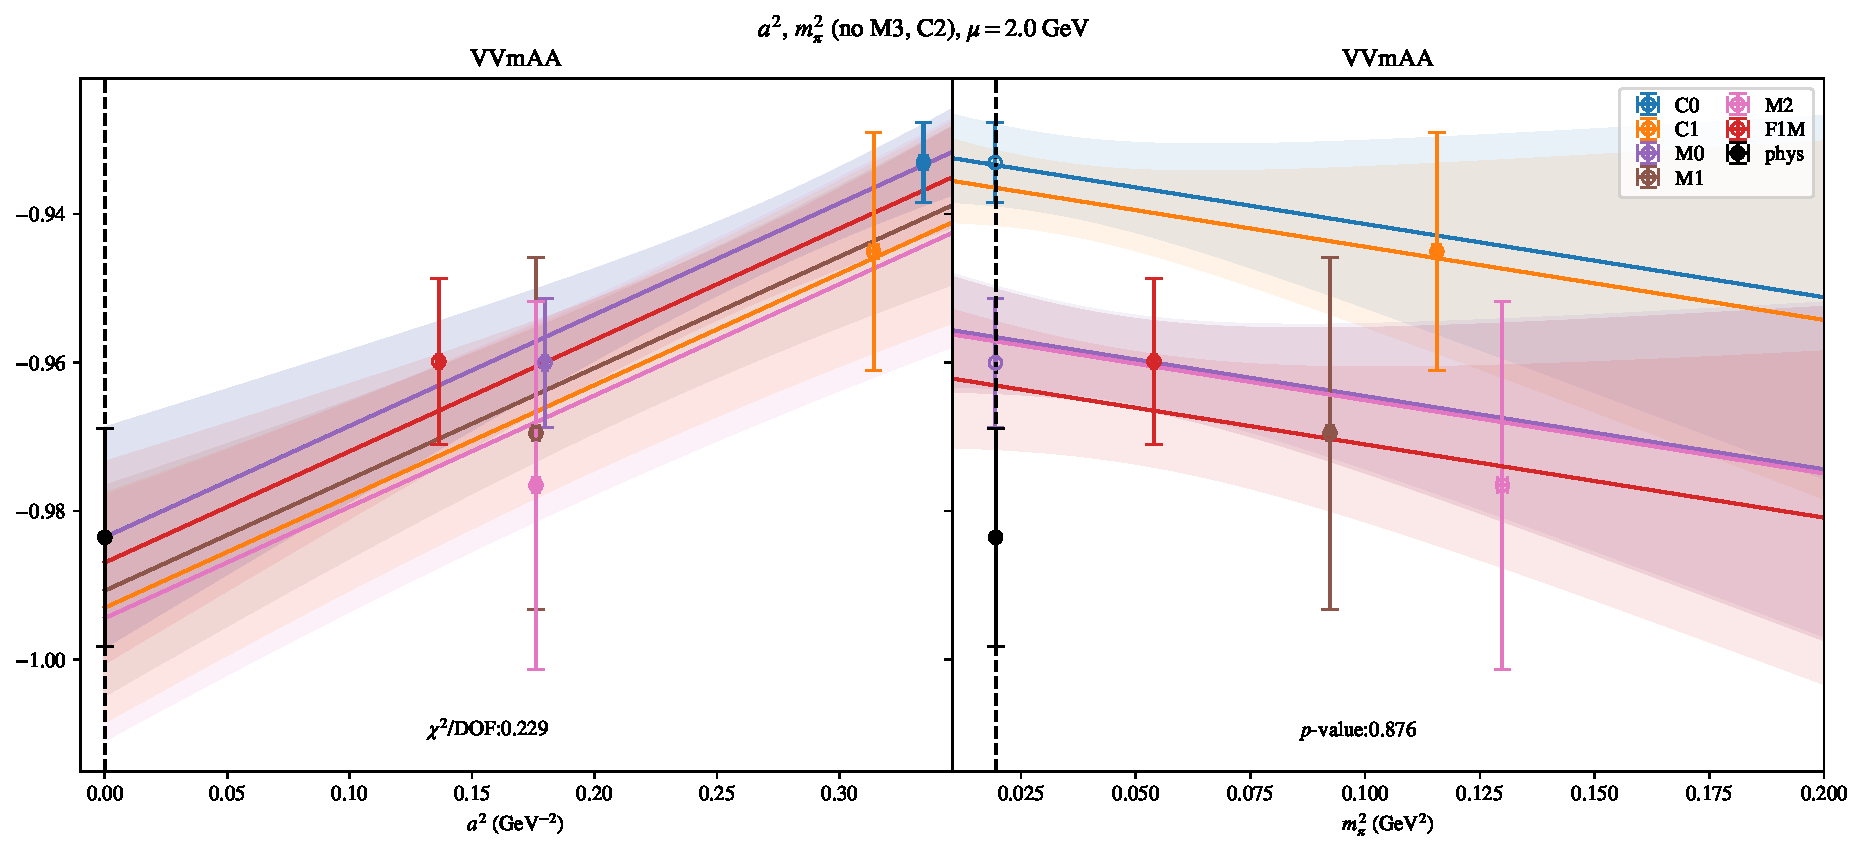
\includepdf[link, pages=-]{VVmAA/NPR/bag_a2m2mcut_20.pdf}
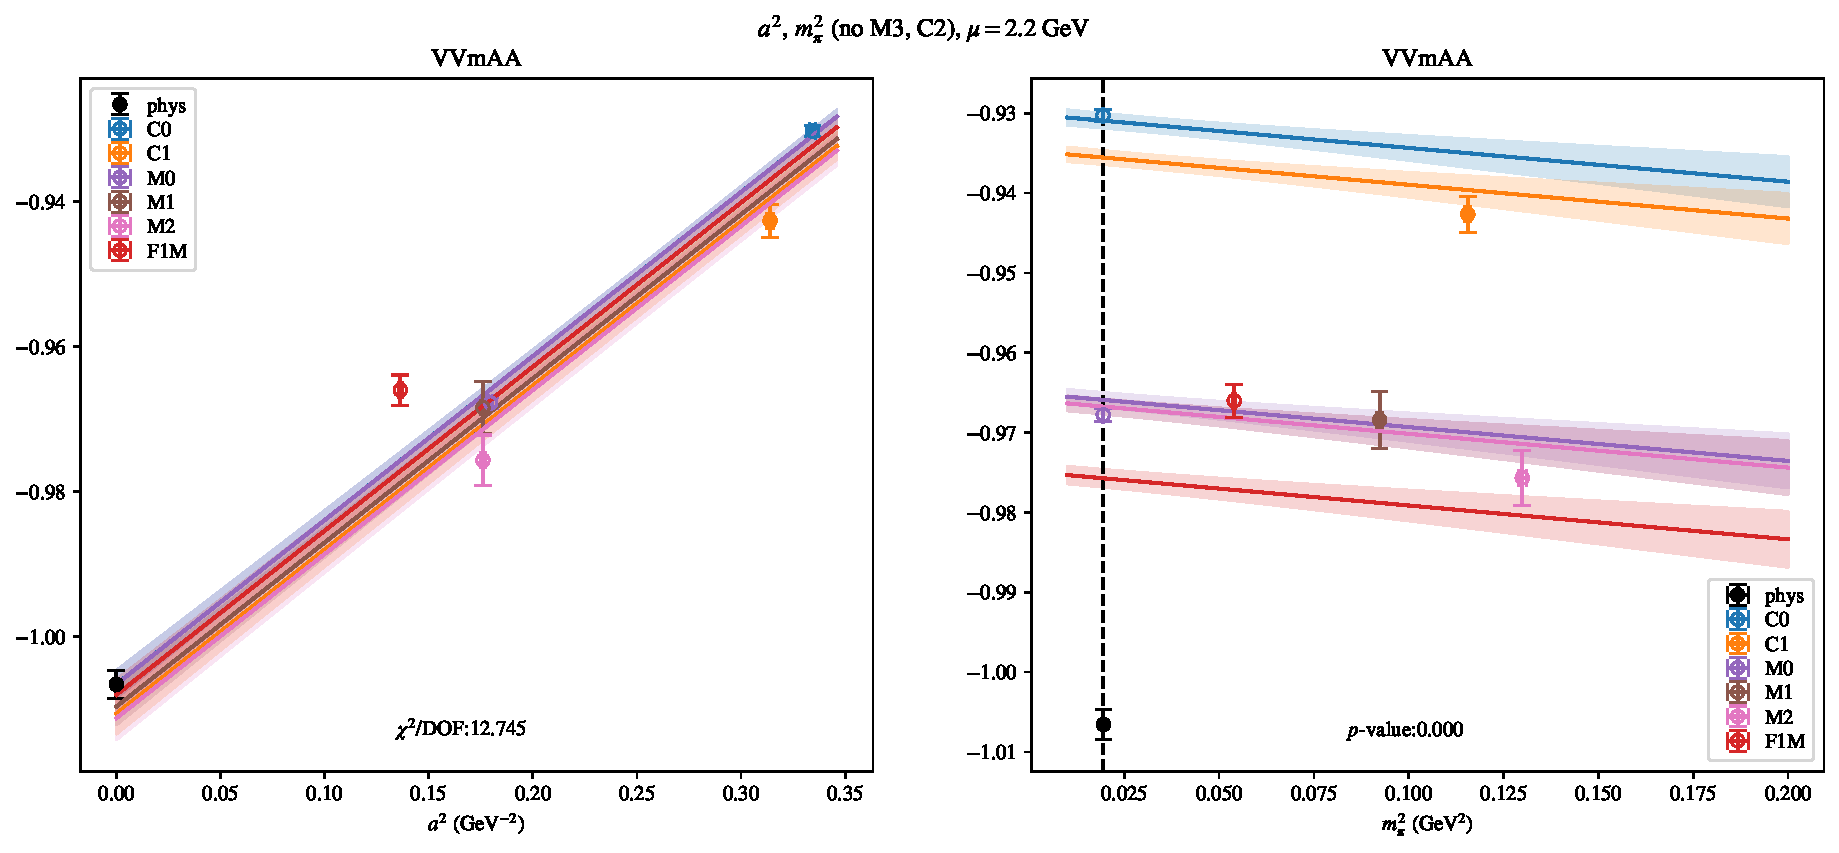
\includepdf[link, pages=-]{VVmAA/NPR/bag_a2m2mcut_22.pdf}
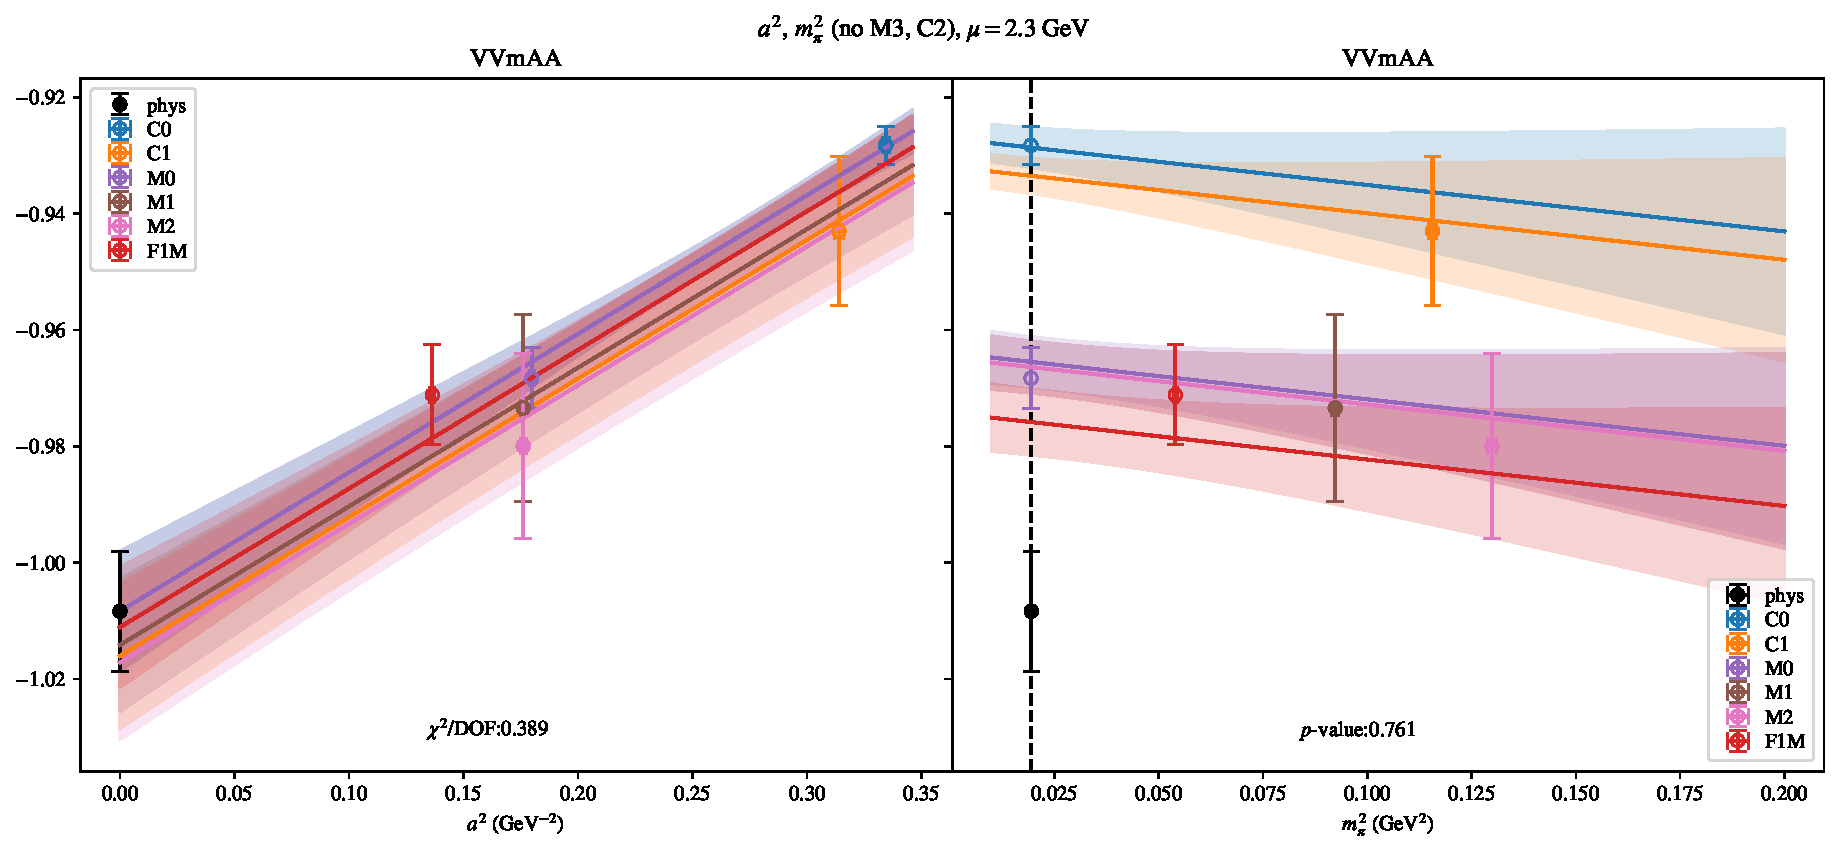
\includepdf[link, pages=-]{VVmAA/NPR/bag_a2m2mcut_23.pdf}
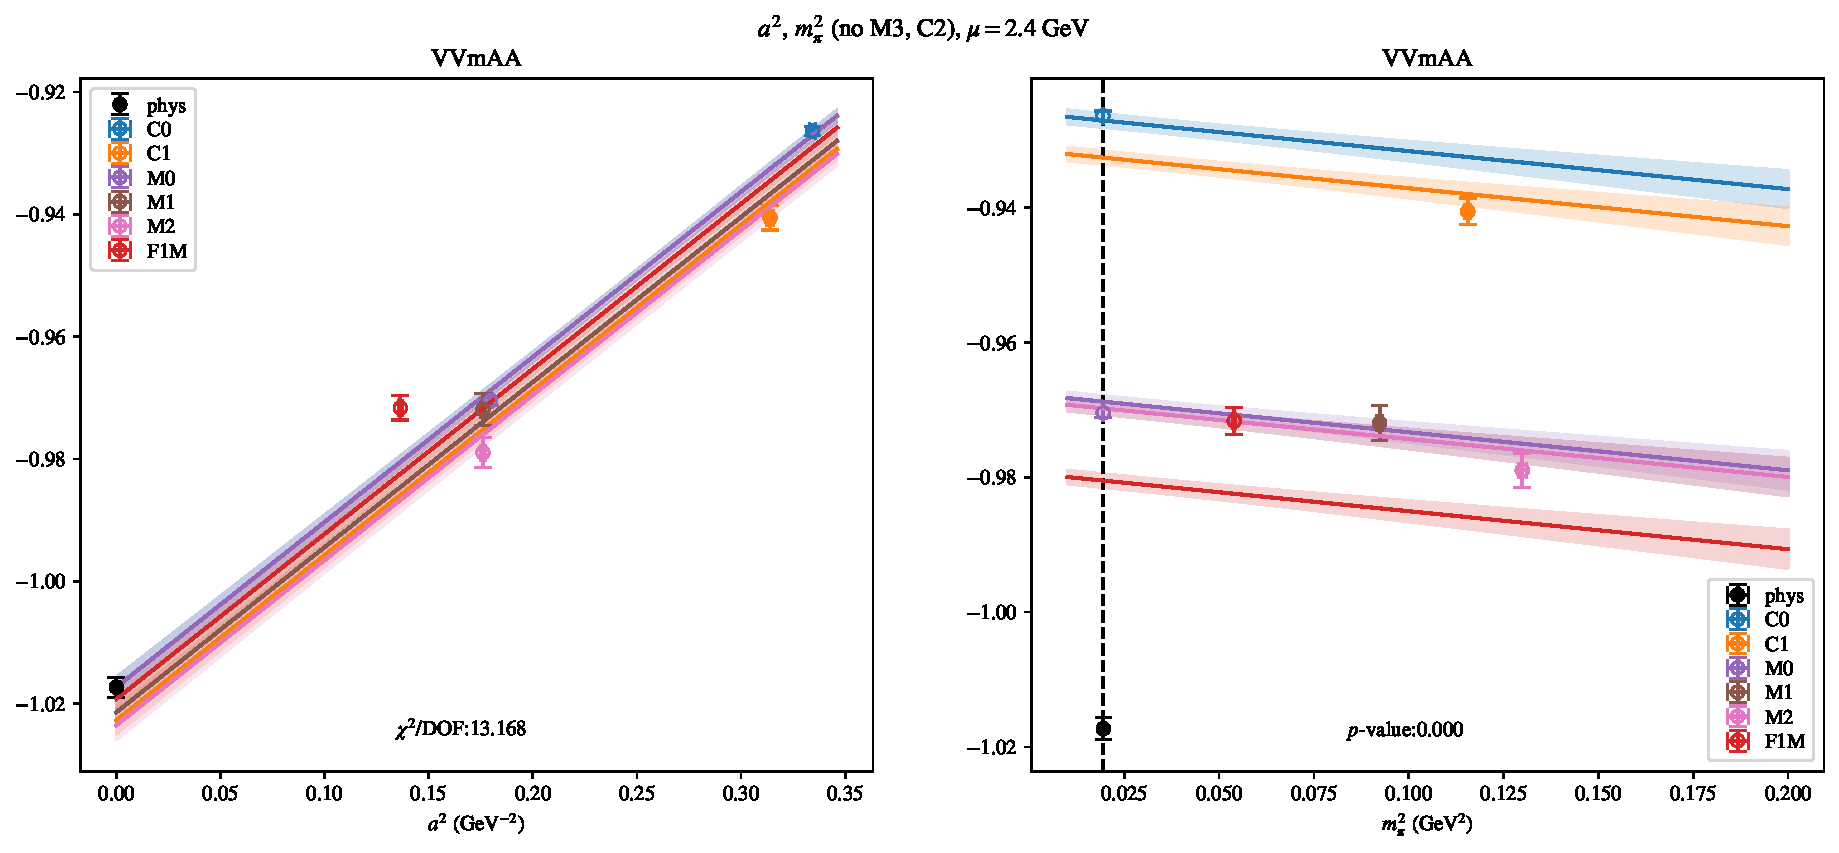
\includepdf[link, pages=-]{VVmAA/NPR/bag_a2m2mcut_24.pdf}
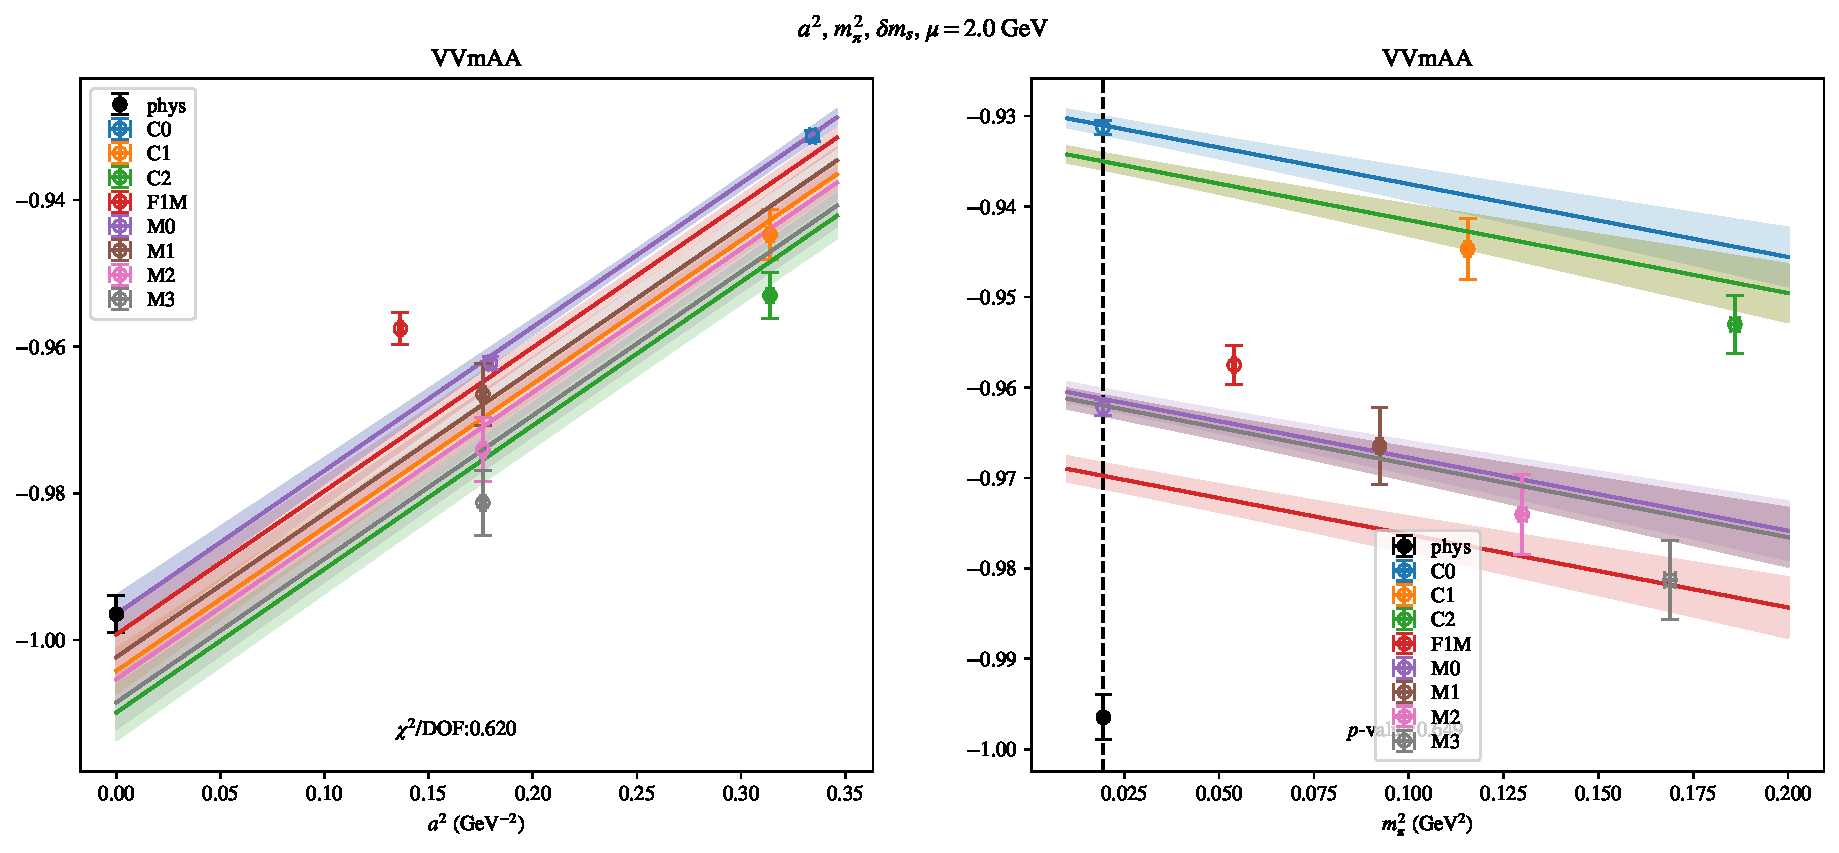
\includepdf[link, pages=-]{VVmAA/NPR/bag_a2m2delm_20.pdf}
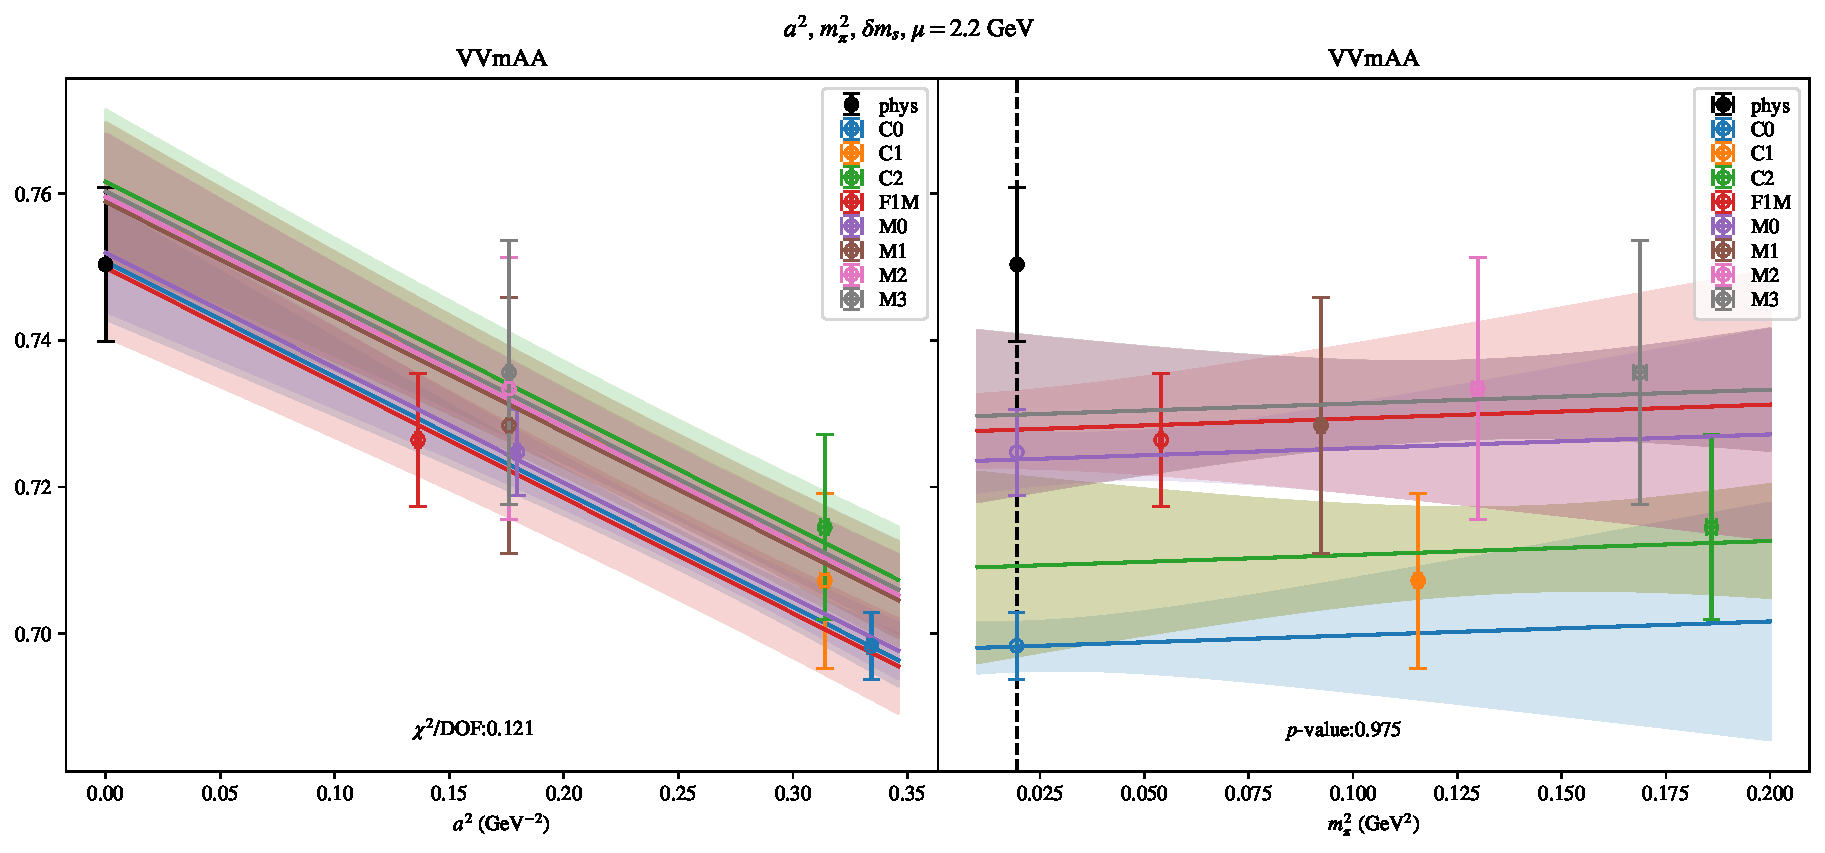
\includepdf[link, pages=-]{VVmAA/NPR/bag_a2m2delm_22.pdf}
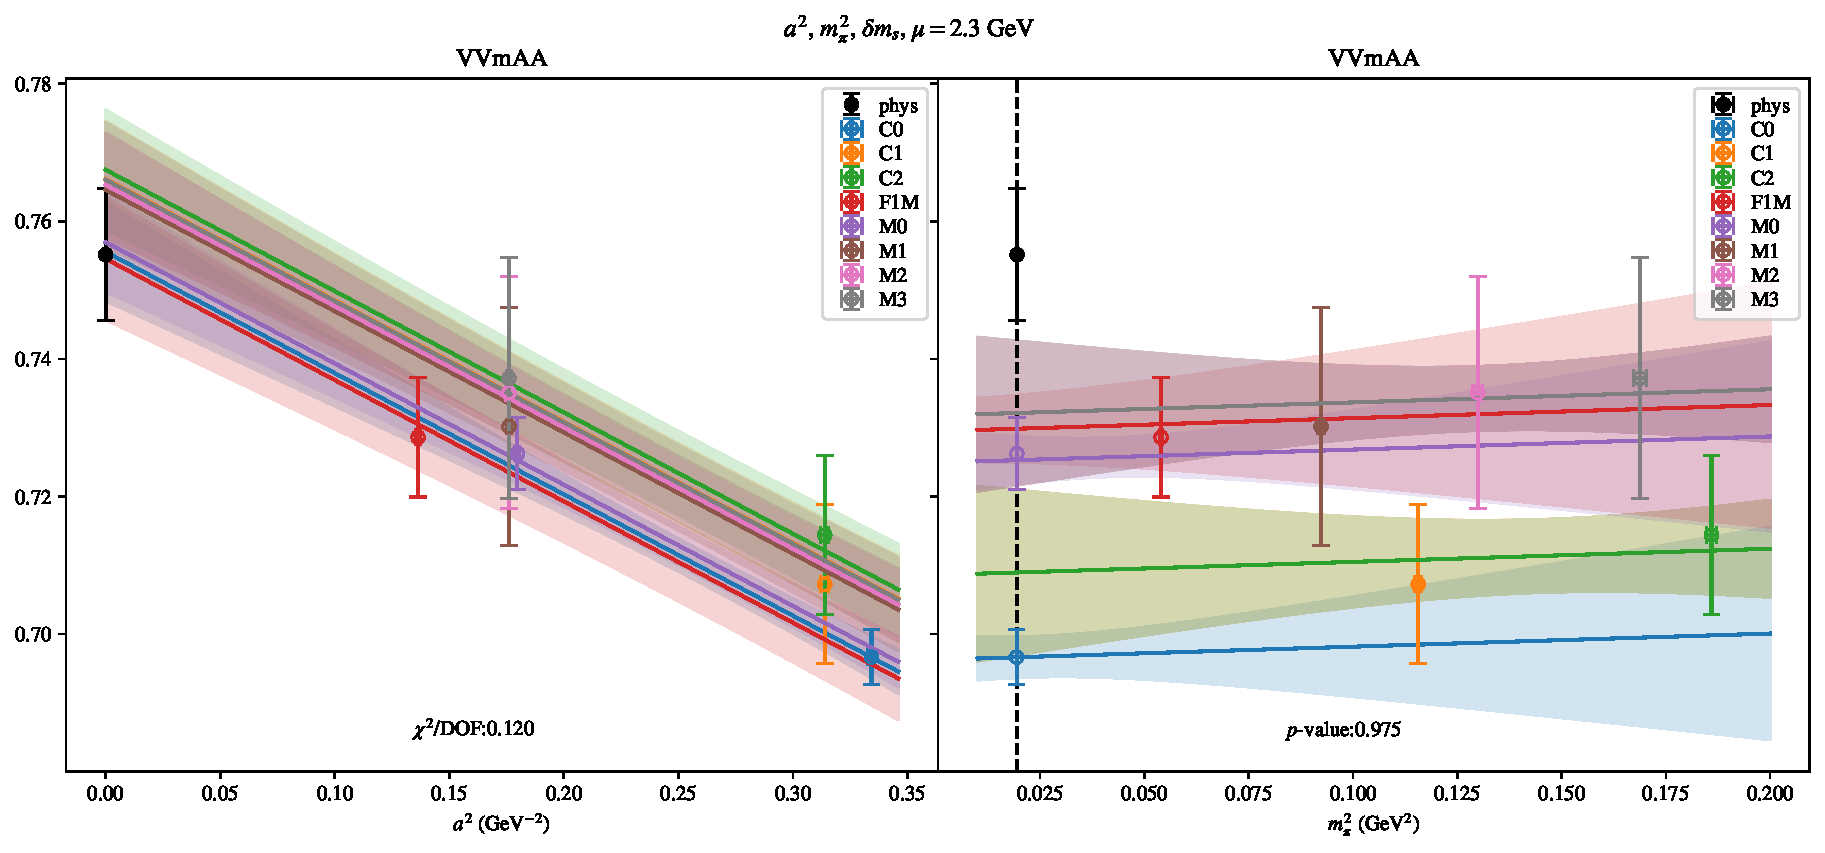
\includepdf[link, pages=-]{VVmAA/NPR/bag_a2m2delm_23.pdf}
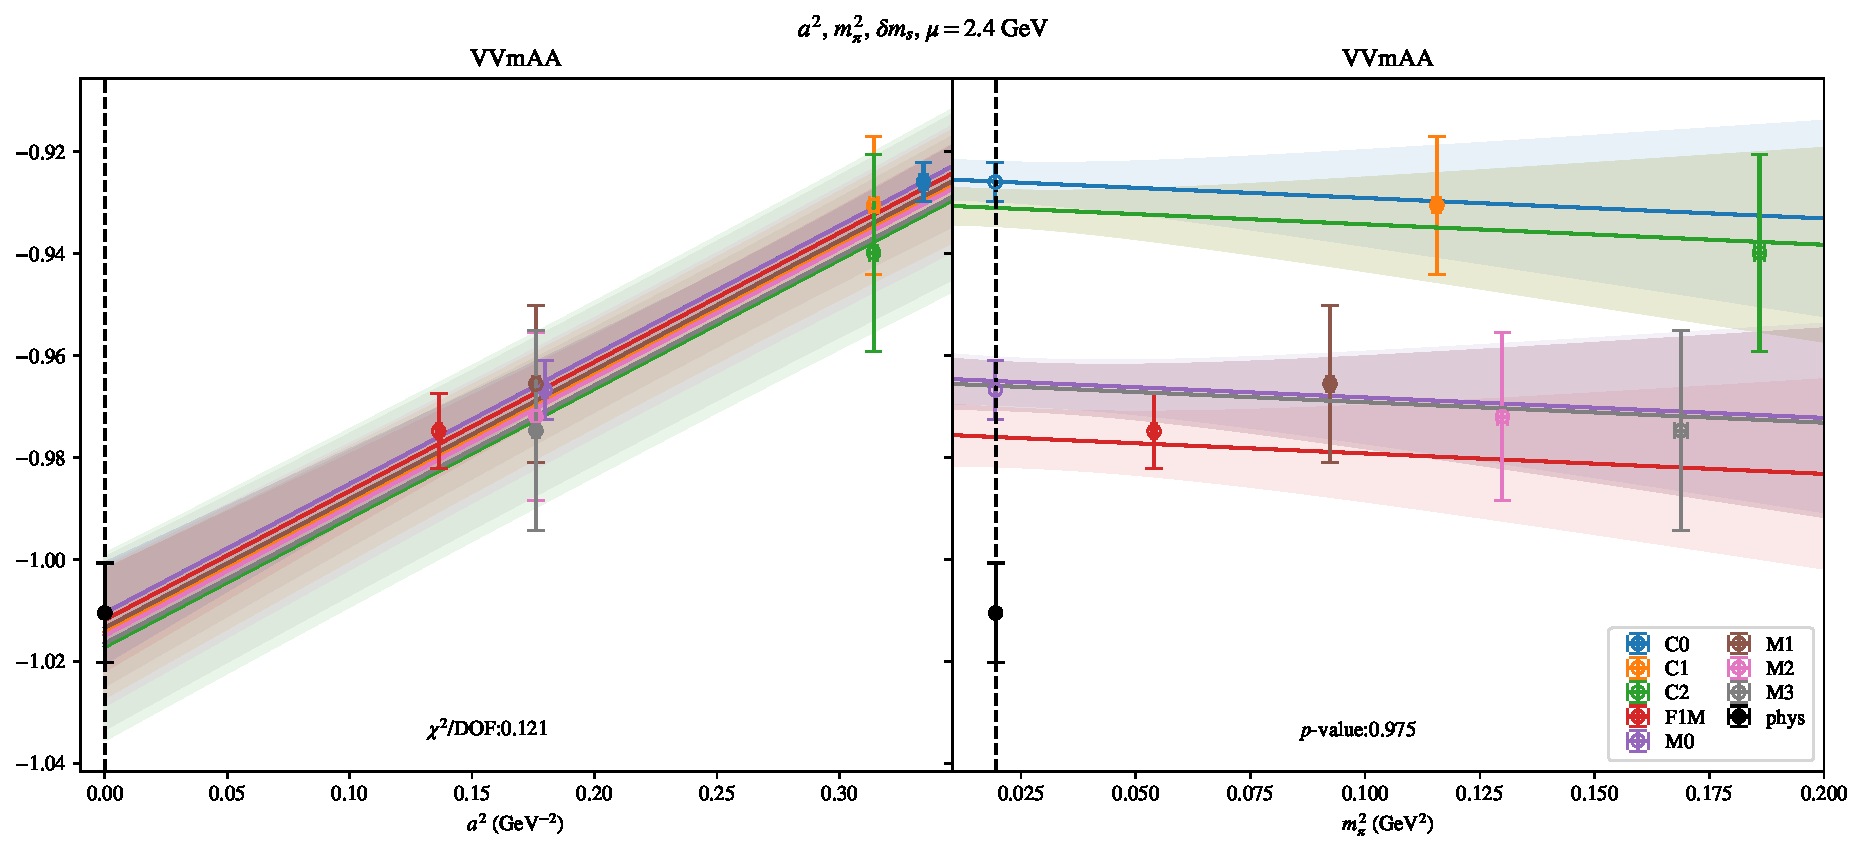
\includepdf[link, pages=-]{VVmAA/NPR/bag_a2m2delm_24.pdf}
\clearpage
\section{$\mathcal{B}_3$}
\begin{table}[h!]
\begin{center}
\begin{tabular}{|c|c|c|c|c|c|}
\hline
$\mu$ (GeV) & $a^2$, $m_\pi^2$& $a^2$, $m_\pi^2$ (no C)& $a^2$, $m_\pi^2$, $a^4$& $a^2$, $m_\pi^2$ (no M3, C2)& $a^2$, $m_\pi^2$, $\delta m_s$\\
\hline
2.0& \hyperlink{SSmPP/NPR/bag_a2m2_20.pdf.1}{\textbf{1.7963(44)}: 4.343 (0.001)} & \hyperlink{SSmPP/NPR/bag_a2m2noC_20.pdf.1}{\textbf{1.695(22)}: 0.062 (0.94)} & \hyperlink{SSmPP/NPR/bag_a2a4m2_20.pdf.1}{\textbf{1.654(35)}: 1.208 (0.305)} & \hyperlink{SSmPP/NPR/bag_a2m2mcut_20.pdf.1}{\textbf{1.7961(46)}: 6.831 (0.0)} & \hyperlink{SSmPP/NPR/bag_a2m2delm_20.pdf.1}{\textbf{1.7927(51)}: 2.372 (0.05)}\\
2.2& \hyperlink{SSmPP/NPR/bag_a2m2_22.pdf.1}{\textbf{1.7998(36)}: 6.76 (0.0)} & \hyperlink{SSmPP/NPR/bag_a2m2noC_22.pdf.1}{\textbf{1.714(15)}: 0.136 (0.873)} & \hyperlink{SSmPP/NPR/bag_a2a4m2_22.pdf.1}{\textbf{1.664(25)}: 1.15 (0.331)} & \hyperlink{SSmPP/NPR/bag_a2m2mcut_22.pdf.1}{\textbf{1.8005(39)}: 10.637 (0.0)} & \hyperlink{SSmPP/NPR/bag_a2m2delm_22.pdf.1}{\textbf{1.7998(42)}: 4.044 (0.003)}\\
2.3& \hyperlink{SSmPP/NPR/bag_a2m2_23.pdf.1}{\textbf{1.8012(35)}: 7.247 (0.0)} & \hyperlink{SSmPP/NPR/bag_a2m2noC_23.pdf.1}{\textbf{1.719(14)}: 0.162 (0.851)} & \hyperlink{SSmPP/NPR/bag_a2a4m2_23.pdf.1}{\textbf{1.666(24)}: 0.832 (0.505)} & \hyperlink{SSmPP/NPR/bag_a2m2mcut_23.pdf.1}{\textbf{1.8019(38)}: 11.66 (0.0)} & \hyperlink{SSmPP/NPR/bag_a2m2delm_23.pdf.1}{\textbf{1.8013(41)}: 4.032 (0.003)}\\
2.4& \hyperlink{SSmPP/NPR/bag_a2m2_24.pdf.1}{\textbf{1.8035(34)}: 6.533 (0.0)} & \hyperlink{SSmPP/NPR/bag_a2m2noC_24.pdf.1}{\textbf{1.722(14)}: 0.201 (0.818)} & \hyperlink{SSmPP/NPR/bag_a2a4m2_24.pdf.1}{\textbf{1.673(25)}: 0.999 (0.407)} & \hyperlink{SSmPP/NPR/bag_a2m2mcut_24.pdf.1}{\textbf{1.8037(38)}: 10.671 (0.0)} & \hyperlink{SSmPP/NPR/bag_a2m2delm_24.pdf.1}{\textbf{1.8028(39)}: 4.135 (0.002)}\\
\hline
\end{tabular}
\caption{Physical point value from chiral and continuum extrapolation at renormalisation scale $\mu$. Entries are \textbf{value(error)}: $\chi^2/\text{DOF}$ ($p$-value).}
\end{center}
\end{table}
\begin{table}[h!]
\begin{center}
\begin{tabular}{|c c|c|c|c|c|c|}
\hline
$\mu$ (GeV) &  & $a^2$, $m_\pi^2$& $a^2$, $m_\pi^2$ (no C)& $a^2$, $m_\pi^2$, $a^4$& $a^2$, $m_\pi^2$ (no M3, C2)& $a^2$, $m_\pi^2$, $\delta m_s$\\
\hline
\multirow{3}{0.5in}{2.0} & $\alpha$ & 0.146(17)& 0.72(12)& 1.41(31)& 0.147(18)& 0.148(19)\\
 & $\beta$ & -0.00047(44)& 0.00059(81)& -0.00080(45)& -0.00094(76)& -0.00321(90)\\
 & $\gamma$ &  &  & -2.54(62)&  & 0.113(32)\\
\hline
\multirow{3}{0.5in}{2.2} & $\alpha$ & 0.154(13)& 0.663(89)& 1.40(23)& 0.153(14)& 0.147(15)\\
 & $\beta$ & -0.00065(32)& -0.00039(61)& -0.00122(35)& -0.00117(56)& -0.00315(71)\\
 & $\gamma$ &  &  & -2.52(47)&  & 0.098(23)\\
\hline
\multirow{3}{0.5in}{2.3} & $\alpha$ & 0.158(13)& 0.653(83)& 1.41(22)& 0.157(13)& 0.151(15)\\
 & $\beta$ & -0.00038(29)& -0.00034(57)& -0.00095(31)& -0.00079(50)& -0.00286(65)\\
 & $\gamma$ &  &  & -2.53(44)&  & 0.097(22)\\
\hline
\multirow{3}{0.5in}{2.4} & $\alpha$ & 0.158(13)& 0.640(85)& 1.35(22)& 0.158(14)& 0.154(14)\\
 & $\beta$ & -0.00025(26)& -0.00020(51)& -0.00081(29)& -0.00048(46)& -0.00239(63)\\
 & $\gamma$ &  &  & -2.42(45)&  & 0.085(21)\\
\hline
\end{tabular}
\caption{Fit values of coefficients in $Q = Q_{phys} + \mathbf{\alpha} a^2 + \mathbf{\beta}\left(\frac{m_\pi^2}{f_\pi^2}-\frac{m_{\pi,PDG}^2}{f_\pi^2}\right) + \gamma(\ldots)$}
\end{center}
\end{table}
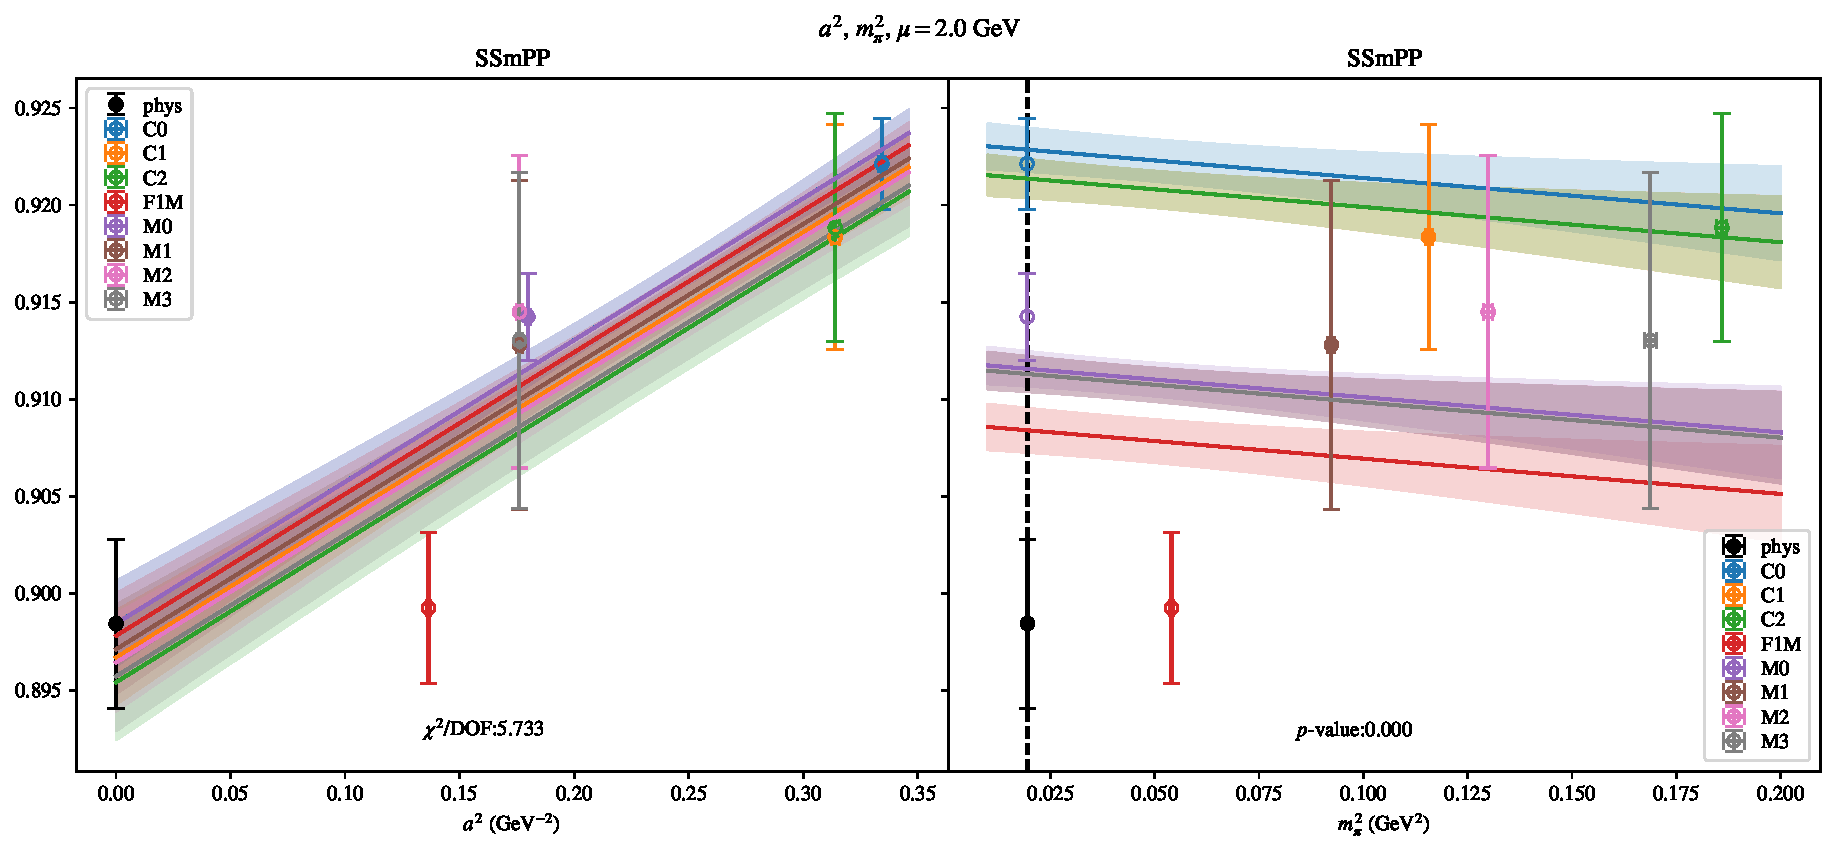
\includepdf[link, pages=-]{SSmPP/NPR/bag_a2m2_20.pdf}
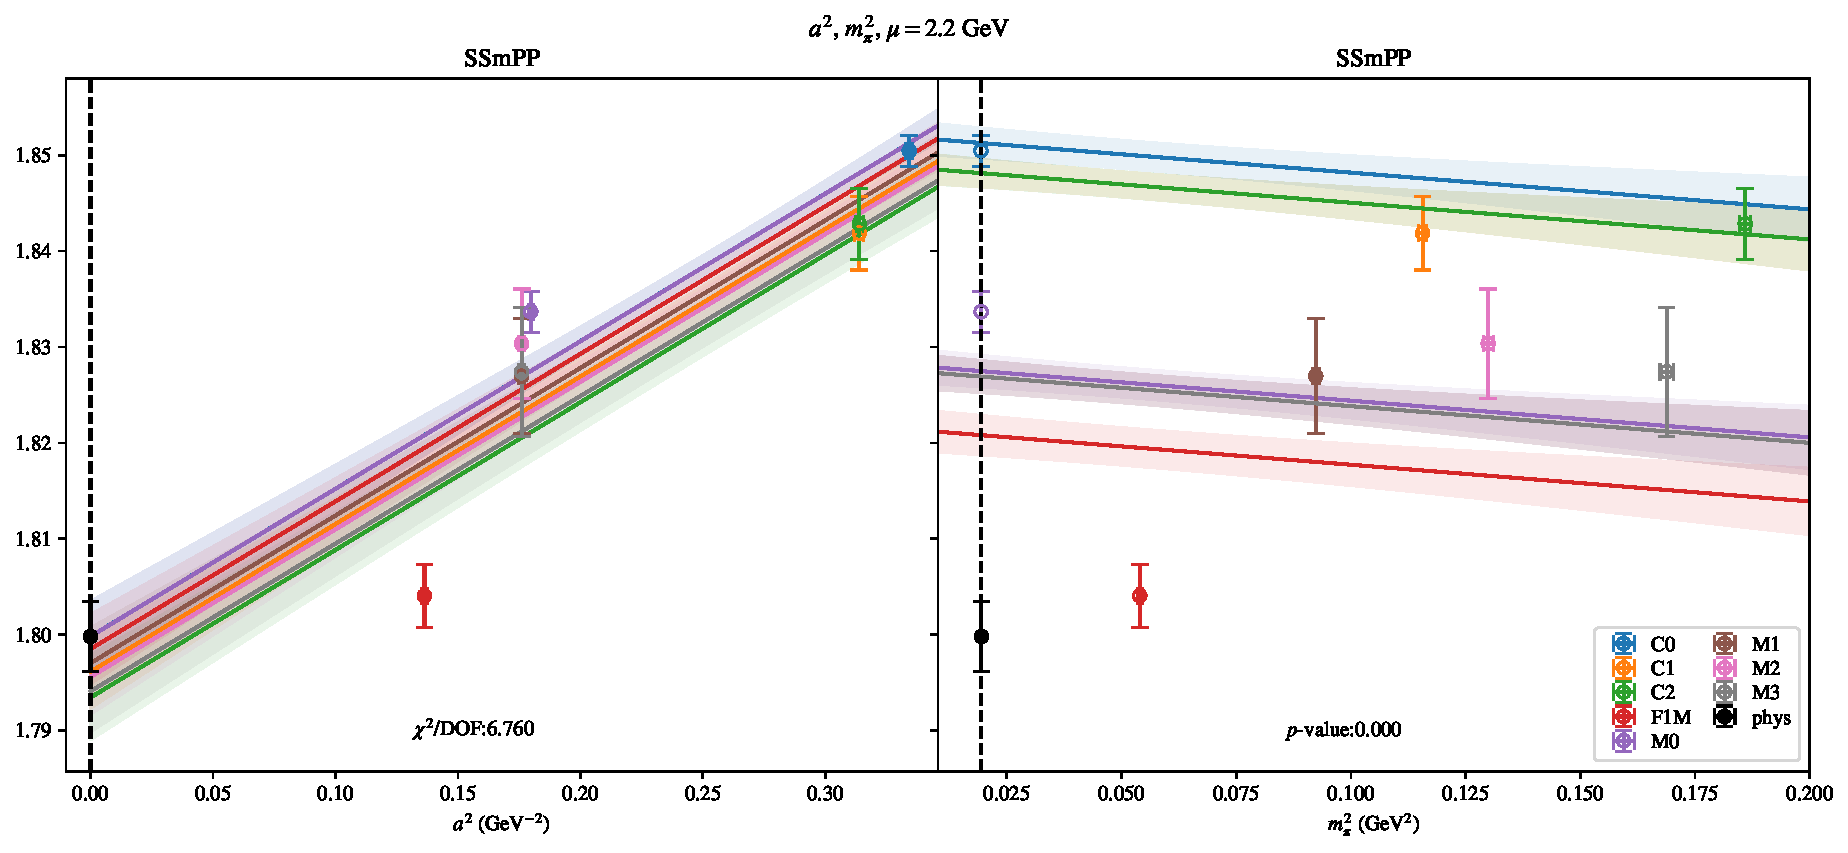
\includepdf[link, pages=-]{SSmPP/NPR/bag_a2m2_22.pdf}
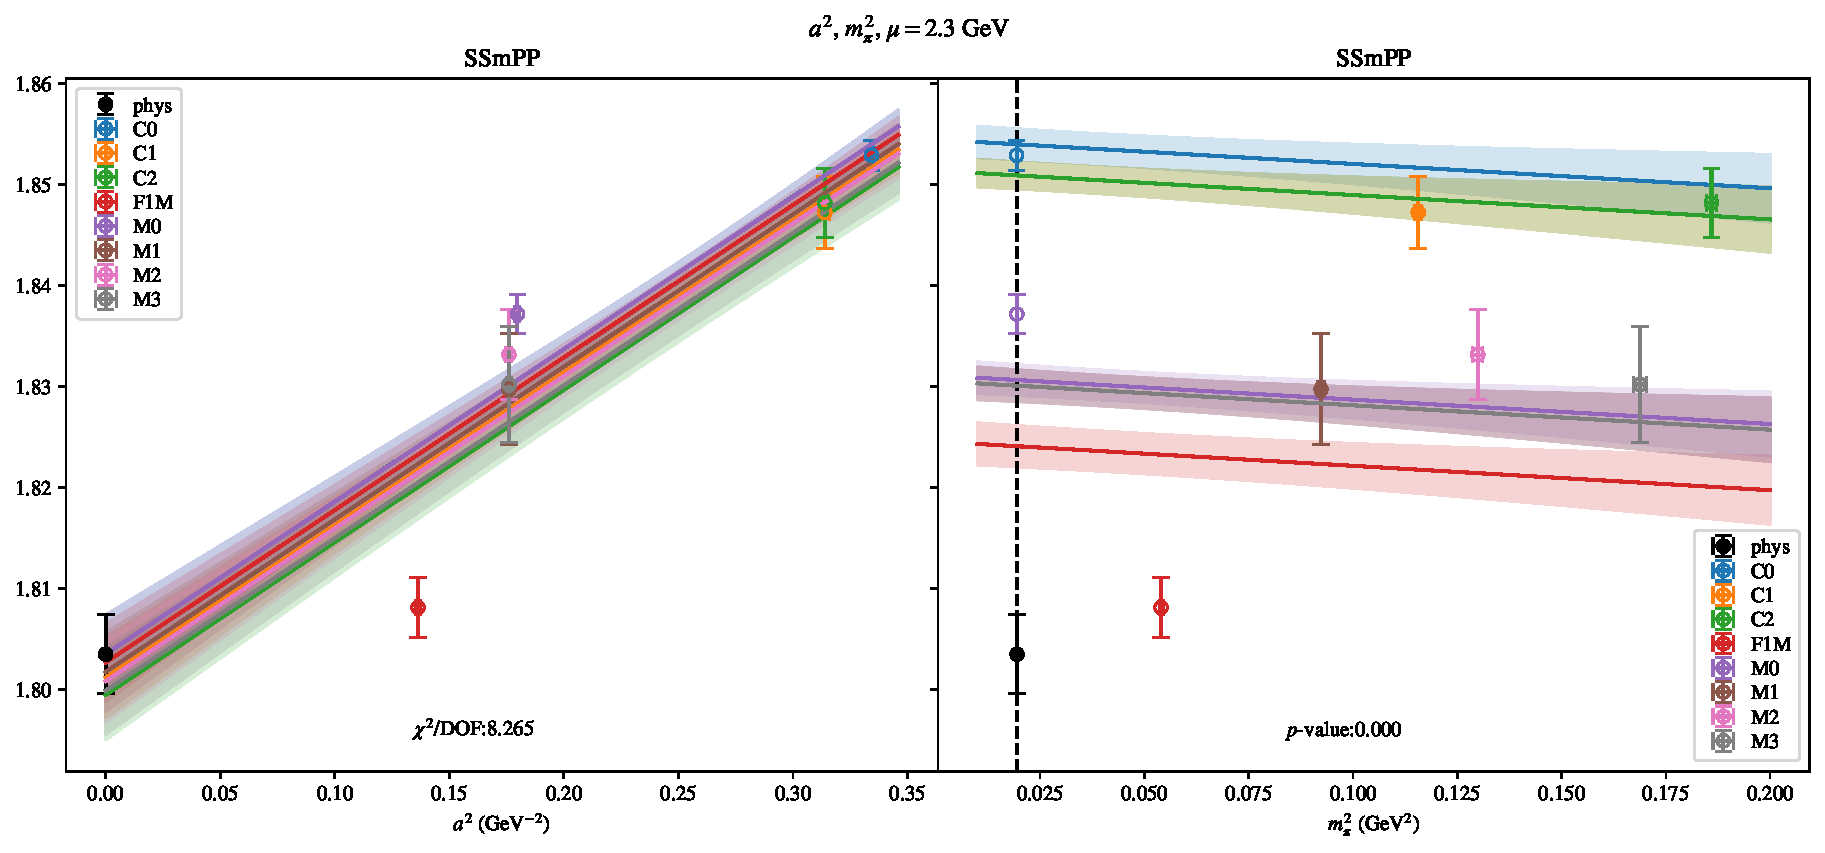
\includepdf[link, pages=-]{SSmPP/NPR/bag_a2m2_23.pdf}
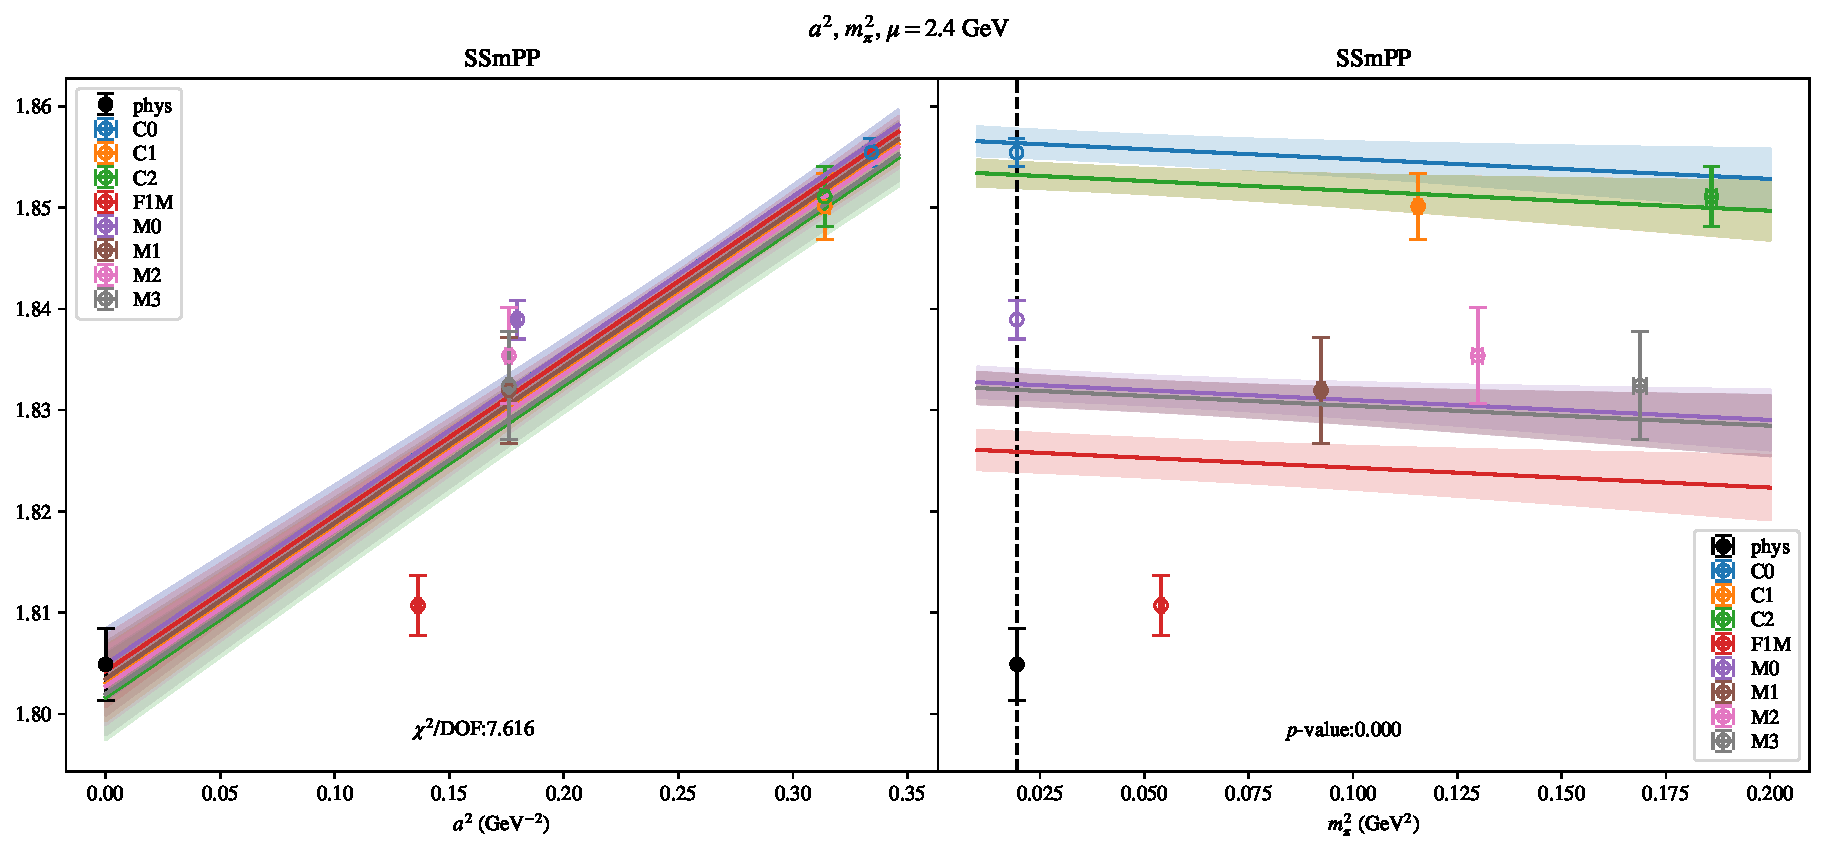
\includepdf[link, pages=-]{SSmPP/NPR/bag_a2m2_24.pdf}
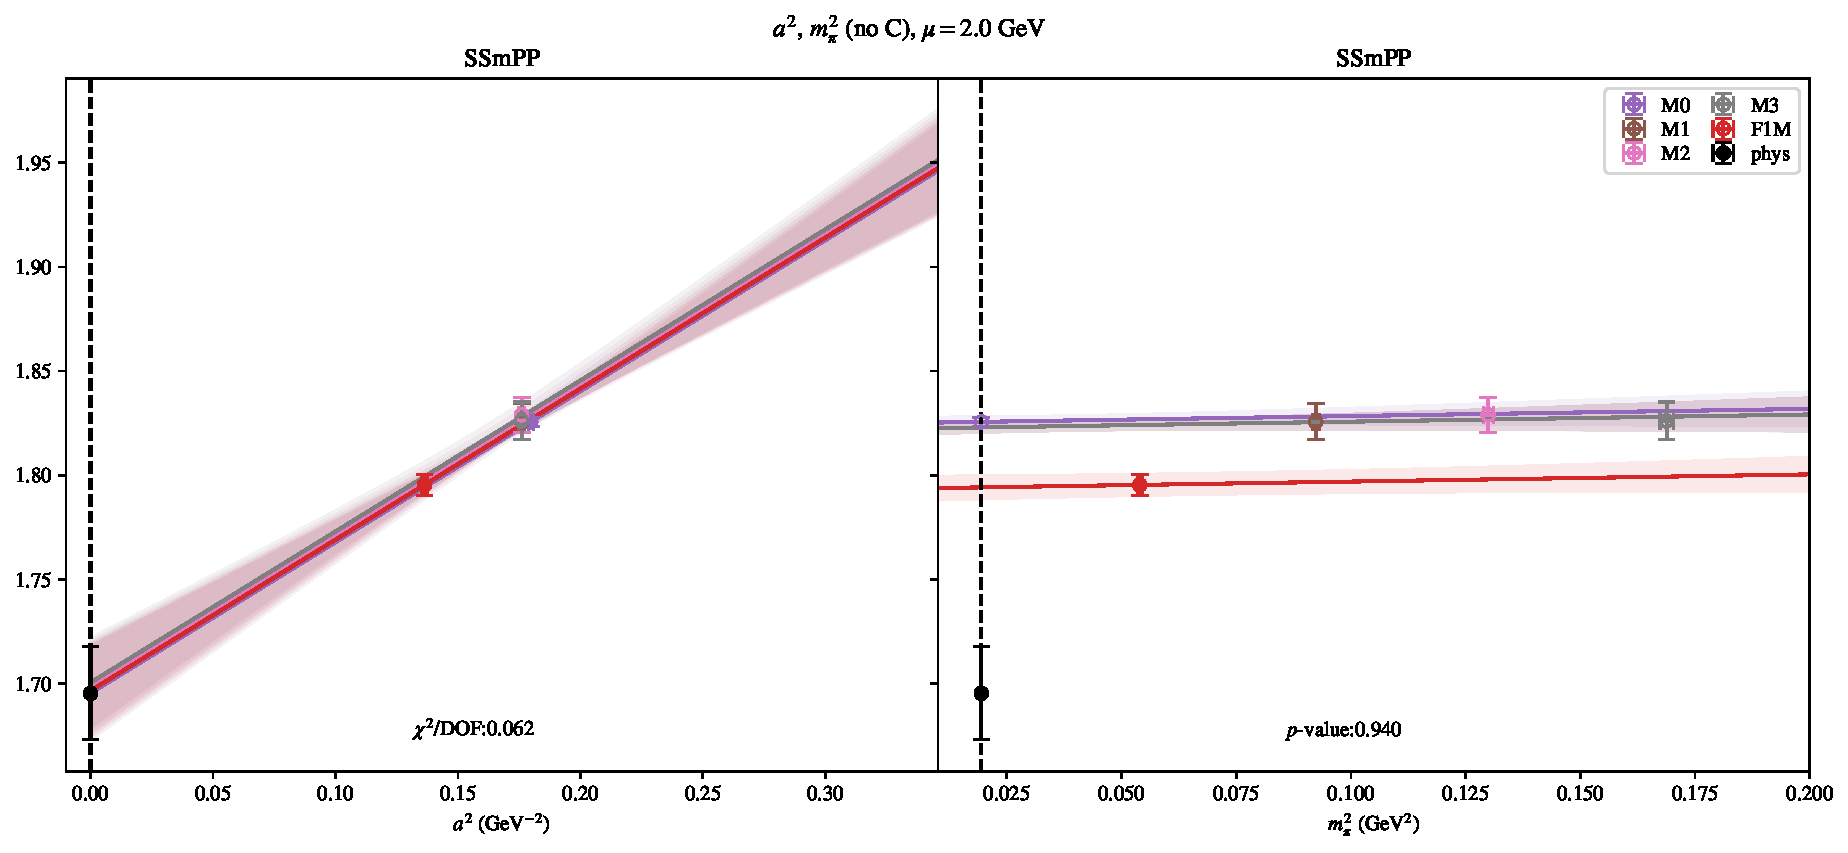
\includepdf[link, pages=-]{SSmPP/NPR/bag_a2m2noC_20.pdf}
\includepdf[link, pages=-]{SSmPP/NPR/bag_a2m2noC_22.pdf}
\includepdf[link, pages=-]{SSmPP/NPR/bag_a2m2noC_23.pdf}
\includepdf[link, pages=-]{SSmPP/NPR/bag_a2m2noC_24.pdf}
\includepdf[link, pages=-]{SSmPP/NPR/bag_a2a4m2_20.pdf}
\includepdf[link, pages=-]{SSmPP/NPR/bag_a2a4m2_22.pdf}
\includepdf[link, pages=-]{SSmPP/NPR/bag_a2a4m2_23.pdf}
\includepdf[link, pages=-]{SSmPP/NPR/bag_a2a4m2_24.pdf}
\includepdf[link, pages=-]{SSmPP/NPR/bag_a2m2mcut_20.pdf}
\includepdf[link, pages=-]{SSmPP/NPR/bag_a2m2mcut_22.pdf}
\includepdf[link, pages=-]{SSmPP/NPR/bag_a2m2mcut_23.pdf}
\includepdf[link, pages=-]{SSmPP/NPR/bag_a2m2mcut_24.pdf}
\includepdf[link, pages=-]{SSmPP/NPR/bag_a2m2delm_20.pdf}
\includepdf[link, pages=-]{SSmPP/NPR/bag_a2m2delm_22.pdf}
\includepdf[link, pages=-]{SSmPP/NPR/bag_a2m2delm_23.pdf}
\includepdf[link, pages=-]{SSmPP/NPR/bag_a2m2delm_24.pdf}
\clearpage
\section{$\mathcal{B}_4$}
\begin{table}[h!]
\begin{center}
\begin{tabular}{|c|c|c|c|c|c|}
\hline
$\mu$ (GeV) & $a^2$, $m_\pi^2$& $a^2$, $m_\pi^2$ (no C)& $a^2$, $m_\pi^2$, $a^4$& $a^2$, $m_\pi^2$ (no M3, C2)& $a^2$, $m_\pi^2$, $\delta m_s$\\
\hline
2.0& \hyperlink{SSpPP/NPR/bag_a2m2_20.pdf.1}{\textbf{-0.9238(27)}: 1.157 (0.328)} & \hyperlink{SSpPP/NPR/bag_a2m2noC_20.pdf.1}{\textbf{-0.939(12)}: 0.927 (0.396)} & \hyperlink{SSpPP/NPR/bag_a2a4m2_20.pdf.1}{\textbf{-0.950(19)}: 0.963 (0.426)} & \hyperlink{SSpPP/NPR/bag_a2m2mcut_20.pdf.1}{\textbf{-0.9227(28)}: 0.756 (0.519)} & \hyperlink{SSpPP/NPR/bag_a2m2delm_20.pdf.1}{\textbf{-0.9239(27)}: 1.407 (0.229)}\\
2.2& \hyperlink{SSpPP/NPR/bag_a2m2_22.pdf.1}{\textbf{-0.9065(23)}: 2.065 (0.067)} & \hyperlink{SSpPP/NPR/bag_a2m2noC_22.pdf.1}{\textbf{-0.9267(93)}: 0.95 (0.387)} & \hyperlink{SSpPP/NPR/bag_a2a4m2_22.pdf.1}{\textbf{-0.932(15)}: 1.863 (0.114)} & \hyperlink{SSpPP/NPR/bag_a2m2mcut_22.pdf.1}{\textbf{-0.9057(24)}: 1.914 (0.125)} & \hyperlink{SSpPP/NPR/bag_a2m2delm_22.pdf.1}{\textbf{-0.9065(22)}: 2.535 (0.038)}\\
2.3& \hyperlink{SSpPP/NPR/bag_a2m2_23.pdf.1}{\textbf{-0.8976(22)}: 2.93 (0.012)} & \hyperlink{SSpPP/NPR/bag_a2m2noC_23.pdf.1}{\textbf{-0.9193(84)}: 1.205 (0.3)} & \hyperlink{SSpPP/NPR/bag_a2a4m2_23.pdf.1}{\textbf{-0.924(14)}: 2.761 (0.026)} & \hyperlink{SSpPP/NPR/bag_a2m2mcut_23.pdf.1}{\textbf{-0.8969(23)}: 2.987 (0.03)} & \hyperlink{SSpPP/NPR/bag_a2m2delm_23.pdf.1}{\textbf{-0.8976(21)}: 3.59 (0.006)}\\
2.4& \hyperlink{SSpPP/NPR/bag_a2m2_24.pdf.1}{\textbf{-0.8891(21)}: 3.493 (0.004)} & \hyperlink{SSpPP/NPR/bag_a2m2noC_24.pdf.1}{\textbf{-0.9121(86)}: 1.456 (0.233)} & \hyperlink{SSpPP/NPR/bag_a2a4m2_24.pdf.1}{\textbf{-0.915(15)}: 3.534 (0.007)} & \hyperlink{SSpPP/NPR/bag_a2m2mcut_24.pdf.1}{\textbf{-0.8886(22)}: 3.694 (0.011)} & \hyperlink{SSpPP/NPR/bag_a2m2delm_24.pdf.1}{\textbf{-0.8892(21)}: 4.352 (0.002)}\\
\hline
\end{tabular}
\caption{Physical point value from chiral and continuum extrapolation at renormalisation scale $\mu$. Entries are \textbf{value(error)}: $\chi^2/\text{DOF}$ ($p$-value).}
\end{center}
\end{table}
\begin{table}[h!]
\begin{center}
\begin{tabular}{|c c|c|c|c|c|c|}
\hline
$\mu$ (GeV) &  & $a^2$, $m_\pi^2$& $a^2$, $m_\pi^2$ (no C)& $a^2$, $m_\pi^2$, $a^4$& $a^2$, $m_\pi^2$ (no M3, C2)& $a^2$, $m_\pi^2$, $\delta m_s$\\
\hline
\multirow{3}{0.5in}{2.0} & $\alpha$ & -0.359(10)& -0.269(68)& -0.13(17)& -0.362(11)& -0.359(10)\\
 & $\beta$ & -0.00710(28)& -0.00722(52)& -0.00715(28)& -0.00783(48)& -0.00728(50)\\
 & $\gamma$ &  &  & -0.47(34)&  & 0.007(17)\\
\hline
\multirow{3}{0.5in}{2.2} & $\alpha$ & -0.3831(85)& -0.265(53)& -0.15(14)& -0.3850(88)& -0.3835(84)\\
 & $\beta$ & -0.00681(19)& -0.00655(38)& -0.00690(20)& -0.00735(33)& -0.00696(38)\\
 & $\gamma$ &  &  & -0.47(28)&  & 0.006(13)\\
\hline
\multirow{3}{0.5in}{2.3} & $\alpha$ & -0.3990(83)& -0.273(48)& -0.16(13)& -0.4005(86)& -0.3995(82)\\
 & $\beta$ & -0.00690(18)& -0.00653(34)& -0.00699(18)& -0.00742(32)& -0.00707(36)\\
 & $\gamma$ &  &  & -0.48(27)&  & 0.007(12)\\
\hline
\multirow{3}{0.5in}{2.4} & $\alpha$ & -0.4156(83)& -0.283(49)& -0.18(13)& -0.4164(85)& -0.4158(82)\\
 & $\beta$ & -0.00688(17)& -0.00648(31)& -0.00697(18)& -0.00736(29)& -0.00695(36)\\
 & $\gamma$ &  &  & -0.47(28)&  & 0.003(12)\\
\hline
\end{tabular}
\caption{Fit values of coefficients in $Q = Q_{phys} + \mathbf{\alpha} a^2 + \mathbf{\beta}\left(\frac{m_\pi^2}{f_\pi^2}-\frac{m_{\pi,PDG}^2}{f_\pi^2}\right) + \gamma(\ldots)$}
\end{center}
\end{table}
\includepdf[link, pages=-]{SSpPP/NPR/bag_a2m2_20.pdf}
\includepdf[link, pages=-]{SSpPP/NPR/bag_a2m2_22.pdf}
\includepdf[link, pages=-]{SSpPP/NPR/bag_a2m2_23.pdf}
\includepdf[link, pages=-]{SSpPP/NPR/bag_a2m2_24.pdf}
\includepdf[link, pages=-]{SSpPP/NPR/bag_a2m2noC_20.pdf}
\includepdf[link, pages=-]{SSpPP/NPR/bag_a2m2noC_22.pdf}
\includepdf[link, pages=-]{SSpPP/NPR/bag_a2m2noC_23.pdf}
\includepdf[link, pages=-]{SSpPP/NPR/bag_a2m2noC_24.pdf}
\includepdf[link, pages=-]{SSpPP/NPR/bag_a2a4m2_20.pdf}
\includepdf[link, pages=-]{SSpPP/NPR/bag_a2a4m2_22.pdf}
\includepdf[link, pages=-]{SSpPP/NPR/bag_a2a4m2_23.pdf}
\includepdf[link, pages=-]{SSpPP/NPR/bag_a2a4m2_24.pdf}
\includepdf[link, pages=-]{SSpPP/NPR/bag_a2m2mcut_20.pdf}
\includepdf[link, pages=-]{SSpPP/NPR/bag_a2m2mcut_22.pdf}
\includepdf[link, pages=-]{SSpPP/NPR/bag_a2m2mcut_23.pdf}
\includepdf[link, pages=-]{SSpPP/NPR/bag_a2m2mcut_24.pdf}
\includepdf[link, pages=-]{SSpPP/NPR/bag_a2m2delm_20.pdf}
\includepdf[link, pages=-]{SSpPP/NPR/bag_a2m2delm_22.pdf}
\includepdf[link, pages=-]{SSpPP/NPR/bag_a2m2delm_23.pdf}
\includepdf[link, pages=-]{SSpPP/NPR/bag_a2m2delm_24.pdf}
\clearpage
\section{$\mathcal{B}_5$}
\begin{table}[h!]
\begin{center}
\begin{tabular}{|c|c|c|c|c|c|}
\hline
$\mu$ (GeV) & $a^2$, $m_\pi^2$& $a^2$, $m_\pi^2$ (no C)& $a^2$, $m_\pi^2$, $a^4$& $a^2$, $m_\pi^2$ (no M3, C2)& $a^2$, $m_\pi^2$, $\delta m_s$\\
\hline
2.0& \hyperlink{TT/NPR/bag_a2m2_20.pdf.1}{\textbf{-0.3624(71)}: 0.026 (1.0)} & \hyperlink{TT/NPR/bag_a2m2noC_20.pdf.1}{\textbf{-0.371(26)}: 0.005 (0.995)} & \hyperlink{TT/NPR/bag_a2a4m2_20.pdf.1}{\textbf{-0.377(44)}: 0.007 (1.0)} & \hyperlink{TT/NPR/bag_a2m2mcut_20.pdf.1}{\textbf{-0.3623(75)}: 0.036 (0.991)} & \hyperlink{TT/NPR/bag_a2m2delm_20.pdf.1}{\textbf{-0.3622(71)}: 0.018 (0.999)}\\
2.2& \hyperlink{TT/NPR/bag_a2m2_22.pdf.1}{\textbf{-0.3603(60)}: 0.039 (0.999)} & \hyperlink{TT/NPR/bag_a2m2noC_22.pdf.1}{\textbf{-0.370(24)}: 0.002 (0.998)} & \hyperlink{TT/NPR/bag_a2a4m2_22.pdf.1}{\textbf{-0.374(41)}: 0.02 (0.999)} & \hyperlink{TT/NPR/bag_a2m2mcut_22.pdf.1}{\textbf{-0.3604(65)}: 0.054 (0.983)} & \hyperlink{TT/NPR/bag_a2m2delm_22.pdf.1}{\textbf{-0.3602(60)}: 0.031 (0.998)}\\
2.3& \hyperlink{TT/NPR/bag_a2m2_23.pdf.1}{\textbf{-0.3591(54)}: 0.047 (0.999)} & \hyperlink{TT/NPR/bag_a2m2noC_23.pdf.1}{\textbf{-0.368(21)}: 0.005 (0.995)} & \hyperlink{TT/NPR/bag_a2a4m2_23.pdf.1}{\textbf{-0.371(37)}: 0.033 (0.998)} & \hyperlink{TT/NPR/bag_a2m2mcut_23.pdf.1}{\textbf{-0.3592(58)}: 0.06 (0.981)} & \hyperlink{TT/NPR/bag_a2m2delm_23.pdf.1}{\textbf{-0.3590(54)}: 0.046 (0.996)}\\
2.4& \hyperlink{TT/NPR/bag_a2m2_24.pdf.1}{\textbf{-0.3580(49)}: 0.056 (0.998)} & \hyperlink{TT/NPR/bag_a2m2noC_24.pdf.1}{\textbf{-0.366(19)}: 0.009 (0.991)} & \hyperlink{TT/NPR/bag_a2a4m2_24.pdf.1}{\textbf{-0.370(34)}: 0.04 (0.997)} & \hyperlink{TT/NPR/bag_a2m2mcut_24.pdf.1}{\textbf{-0.3581(55)}: 0.068 (0.977)} & \hyperlink{TT/NPR/bag_a2m2delm_24.pdf.1}{\textbf{-0.3579(49)}: 0.057 (0.994)}\\
\hline
\end{tabular}
\caption{Physical point value from chiral and continuum extrapolation at renormalisation scale $\mu$. Entries are \textbf{value(error)}: $\chi^2/\text{DOF}$ ($p$-value).}
\end{center}
\end{table}
\begin{table}[h!]
\begin{center}
\begin{tabular}{|c c|c|c|c|c|c|}
\hline
$\mu$ (GeV) &  & $a^2$, $m_\pi^2$& $a^2$, $m_\pi^2$ (no C)& $a^2$, $m_\pi^2$, $a^4$& $a^2$, $m_\pi^2$ (no M3, C2)& $a^2$, $m_\pi^2$, $\delta m_s$\\
\hline
\multirow{3}{0.5in}{2.0} & $\alpha$ & 0.009(24)& 0.06(15)& 0.14(40)& 0.008(26)& 0.007(25)\\
 & $\beta$ & -0.00242(68)& -0.0024(11)& -0.00248(69)& -0.0025(11)& -0.0027(11)\\
 & $\gamma$ &  &  & -0.27(82)&  & 0.011(39)\\
\hline
\multirow{3}{0.5in}{2.2} & $\alpha$ & 0.028(21)& 0.09(14)& 0.16(38)& 0.028(22)& 0.027(21)\\
 & $\beta$ & -0.00229(55)& -0.00216(99)& -0.00235(59)& -0.00234(94)& -0.0026(11)\\
 & $\gamma$ &  &  & -0.26(77)&  & 0.010(35)\\
\hline
\multirow{3}{0.5in}{2.3} & $\alpha$ & 0.036(18)& 0.09(12)& 0.15(33)& 0.036(19)& 0.035(18)\\
 & $\beta$ & -0.00237(54)& -0.00220(90)& -0.00242(57)& -0.00245(88)& -0.0026(10)\\
 & $\gamma$ &  &  & -0.23(68)&  & 0.008(33)\\
\hline
\multirow{3}{0.5in}{2.4} & $\alpha$ & 0.044(17)& 0.09(11)& 0.15(31)& 0.045(18)& 0.043(17)\\
 & $\beta$ & -0.00237(48)& -0.00224(83)& -0.00243(52)& -0.00246(82)& -0.00255(94)\\
 & $\gamma$ &  &  & -0.22(64)&  & 0.007(30)\\
\hline
\end{tabular}
\caption{Fit values of coefficients in $Q = Q_{phys} + \mathbf{\alpha} a^2 + \mathbf{\beta}\left(\frac{m_\pi^2}{f_\pi^2}-\frac{m_{\pi,PDG}^2}{f_\pi^2}\right) + \gamma(\ldots)$}
\end{center}
\end{table}
\includepdf[link, pages=-]{TT/NPR/bag_a2m2_20.pdf}
\includepdf[link, pages=-]{TT/NPR/bag_a2m2_22.pdf}
\includepdf[link, pages=-]{TT/NPR/bag_a2m2_23.pdf}
\includepdf[link, pages=-]{TT/NPR/bag_a2m2_24.pdf}
\includepdf[link, pages=-]{TT/NPR/bag_a2m2noC_20.pdf}
\includepdf[link, pages=-]{TT/NPR/bag_a2m2noC_22.pdf}
\includepdf[link, pages=-]{TT/NPR/bag_a2m2noC_23.pdf}
\includepdf[link, pages=-]{TT/NPR/bag_a2m2noC_24.pdf}
\includepdf[link, pages=-]{TT/NPR/bag_a2a4m2_20.pdf}
\includepdf[link, pages=-]{TT/NPR/bag_a2a4m2_22.pdf}
\includepdf[link, pages=-]{TT/NPR/bag_a2a4m2_23.pdf}
\includepdf[link, pages=-]{TT/NPR/bag_a2a4m2_24.pdf}
\includepdf[link, pages=-]{TT/NPR/bag_a2m2mcut_20.pdf}
\includepdf[link, pages=-]{TT/NPR/bag_a2m2mcut_22.pdf}
\includepdf[link, pages=-]{TT/NPR/bag_a2m2mcut_23.pdf}
\includepdf[link, pages=-]{TT/NPR/bag_a2m2mcut_24.pdf}
\includepdf[link, pages=-]{TT/NPR/bag_a2m2delm_20.pdf}
\includepdf[link, pages=-]{TT/NPR/bag_a2m2delm_22.pdf}
\includepdf[link, pages=-]{TT/NPR/bag_a2m2delm_23.pdf}
\includepdf[link, pages=-]{TT/NPR/bag_a2m2delm_24.pdf}
\clearpage
\end{document}